
\documentclass[twocolumn,epjc]{svjour3}
\pdfoutput=1
\usepackage{lineno}
\usepackage{authblk}
\usepackage[section]{placeins}% to prevent "too many unprocessed floats" error.
\usepackage{subfigure}
\usepackage{tabulary}
\usepackage{booktabs}
\usepackage{mathrsfs}
\usepackage{rotating}
\usepackage{float} 
\usepackage{url}
\usepackage{subfigure}
\usepackage{graphicx}
%\usepackage{caption}
%\usepackage{subcaption}
\usepackage{epstopdf}
\usepackage{rotating}
\usepackage{multirow}
\usepackage{xspace}
\usepackage{hyperref}

%\documentclass[twocolumn,epjc3]{svjour3}  
%
\smartqed  % flush right qed marks, e.g. at end of proof
%
\RequirePackage{graphicx}
\RequirePackage{amssymb}
\RequirePackage{placeins}
\RequirePackage{amsmath}

\graphicspath{ {./Plots/} }

\def\TeV{\ifmmode {\mathrm{\ Te\kern -0.1em V}}\else
                   \textrm{Te\kern -0.1em V}\fi}%
\def\GeV{\ifmmode {\mathrm{\ Ge\kern -0.1em V}}\else
                   \textrm{Ge\kern -0.1em V}\fi}%
\def\MeV{\ifmmode {\mathrm{\ Me\kern -0.1em V}}\else
                   \textrm{Me\kern -0.1em V}\fi}%
\def\keV{\ifmmode {\mathrm{\ ke\kern -0.1em V}}\else
                   \textrm{ke\kern -0.1em V}\fi}%
\def\eV{\ifmmode  {\mathrm{\ e\kern -0.1em V}}\else
                   \textrm{e\kern -0.1em V}\fi}%
\let\tev=\TeV
\let\gev=\GeV
\let\mev=\MeV
\let\kev=\keV
\let\ev=\eV
\def\iab{\mbox{ab$^{-1}$} \xspace}%  Inverse atobarns.
\def\ifb{\mbox{fb$^{-1}$} \xspace}%  Inverse femtobarns.
\def\ipb{\mbox{pb$^{-1}$} \xspace}%  Inverse picobarns.
\def\inb{\mbox{nb$^{-1}$} \xspace}%  Inverse nanobarns.

%\def\Zprime{\mbox{Z'} \xspace}


\newcommand{\Wboson}{\ensuremath{W}}
\newcommand{\Zboson}{\ensuremath{Z}}
\newcommand{\ZprimeM}{\ensuremath{M_{\Zprime}}}


\newcommand{\ttbar}{\ensuremath{t\overline{t}} }
\newcommand{\Zprime}{\ensuremath{Z'} }
\newcommand{\pt}{\ensuremath{p_T} }
\newcommand{\hpp}{\textsc{Herwig}\texttt{++} }
\newcommand{\eq}[1]{Eq.~\eqref{eq:#1}}
\newcommand{\eqs}[2]{Eqs.~\eqref{eq:#1} and \eqref{eq:#2}}
\newcommand{\eqss}[3]{Eqs.~\eqref{eq:#1}, \eqref{eq:#2}, and \eqref{eq:#3}}
\renewcommand{\sec}[1]{Sec.~\ref{sec:#1}}
\newcommand{\secs}[2]{Secs.~\ref{sec:#1} and \ref{sec:#2}}
\newcommand{\subsec}[1]{Sec.~\ref{subsec:#1}}
\newcommand{\subsubsec}[1]{Sec.~\ref{subsubsec:#1}}

\newcommand{\nn}{\nonumber}
\newcommand{\new}{\nn\\}

% text abbrev.
\newcommand{\ie}{i.e.}
\newcommand{\eg}{e.g.}
\newcommand{\cf}{cf.}
\newcommand{\TODO}[1]{\marginpar{\textbf{TODO} \footnotesize{#1}} (\textbf{TODO})}

\newcommand{\figwidth}{0.45\textwidth}
\newcommand{\pythia}  {{\sc Pyth\-ia}}
\newcommand{\pythiasix}  {{\sc Pyth\-ia~6}}
\newcommand{\pythiaeight}  {{\sc Pyth\-ia~8}}
\newcommand{\PYTHIA}{{\sc Py\-thi\-a}}
\newcommand{\ATLAS}{ATLAS}
\newcommand{\CMS}{CMS}
\newcommand{\LHC}{LHC}
\newcommand{\MC}{MC}
\newcommand{\refneeded}{{\bf[REF]}}

\newcommand{\pp}{proton-proton}
\newcommand{\pu}{pile-up}
\newcommand{\PU}{Pile-up}
\newcommand{\pujet}{pile-up jet}
\newcommand{\qcdjet}{QCD jet}
\newcommand{\stojet}{stochastic jet}
\newcommand{\cms}{center-of-mass}
\newcommand{\sqrts}[1]{\ensuremath{\sqrt{s} = #1} \TeV}
\newcommand{\Rpt}{\ensuremath{R_{p_T}}}
\newcommand{\ptmatch}{\ensuremath{p_T^{match}}}
\newcommand{\ptcorr}{\ensuremath{p_T^{corr}}}
\newcommand{\minimumbias}{minimum bias}
\newcommand{\MB}{MB}
\newcommand{\pT}{\ensuremath{p_{\mathrm{T}}}\xspace}
\newcommand{\pTmin}{\ensuremath{p_{\mathrm{T}}^{\mathrm{min}}}}
\newcommand{\pTave}{\ensuremath{\langle\pT\rangle}}
\newcommand{\pseudorapidity}{pseu\-do\-ra\-pi\-di\-ty}
\newcommand{\pseudorapidities}{pseu\-do\-ra\-pi\-di\-ties}
\newcommand{\rap}{\ensuremath{y}}
\newcommand{\prap}{\ensuremath{\eta}}
\newcommand{\azi}{\ensuremath{\phi}}
\newcommand{\etaphispace}{(\prap,\azi) space}
\newcommand{\rapphispace}{(\rap,\azi) space}
\newcommand{\deltaR}{\ensuremath{\Delta R}}
\newcommand{\Rcone}{\ensuremath{R}}
\newcommand{\Rcore}{\ensuremath{R_{\mathrm{core}}}}
\newcommand{\Ecore}{\ensuremath{E_{\mathrm{core}}}}
\newcommand{\Ejet}{\ensuremath{E_{\mathrm{jet}}}}
%\newcommand{\deltaRrap}{\ensuremath{\
\newcommand{\Vprim}{\ensuremath{V_{0}}}

%observables
\newcommand{\ptd}{p_TD}
\newcommand{\C}[2]{C_{#1}^{(#2)}}
\newcommand{\Cnobeta}[1]{C_{#1}}
\newcommand{\zcut}{z_\text{cut}}
\newcommand{\mtrim}{\ensuremath{m_{\mathrm{trim}}}}
\newcommand{\mprun}{\ensuremath{m_{\mathrm{prun}}}}
\newcommand{\mmdt}{\ensuremath{m_{\mathrm{mmdt}}}}
\newcommand{\msd}{\ensuremath{m_{\mathrm{sd}}}}
\newcommand{\wmass}{\ensuremath{m_{W}}}
\newcommand{\topmass}{\ensuremath{m_{t}}}



\newcommand{\Ntrk}{\ensuremath{N_{\mathrm{trk}}}}
\newcommand{\Npart}{\ensuremath{N_{\mathrm{part}}}}
 \newcommand{\coreF}{\ensuremath{\mathcal{F}_{\mathrm{core}}}}

\newcommand{\Nvtx}{\ensuremath{N_{\mathrm{vtx}}}}
\newcommand{\Ncoll}{\ensuremath{N_{\mathrm{coll}}}}
\newcommand{\axing}{\ensuremath{\langle\mu\rangle}}
\newcommand{\jcf}{\ensuremath{\mathcal{F}_{\mathrm{core}}}}
\newcommand{\bjet}{\ensuremath{b}\mbox{-}{\rm jet}}
\newcommand{\FJ}{{\sc Fast\-Jet}}
\newcommand{\JVF}{\ensuremath{\mathcal{F}_{\mathrm{jvf}}}}
%\newcommand{\dfrac}[2]{\frac{\displaystyle{#1}}{\displaystyle{#2}}}

\newcommand{\kT}{\ensuremath{k_{\mathrm{T}}}\xspace}
\newcommand{\antikt}{{\rm anti-}\kT}

% greek
\newcommand{\w}{\omega}
\newcommand{\W}{\Omega}
%\newcommand{\al}{\alpha}
%\newcommand{\ga}{\gamma}
%\newcommand{\de}{\delta}
%\newcommand{\ep}{\epsilon}
%\newcommand{\ze}{\zeta}
%\newcommand{\ka}{\kappa}
%\newcommand{\la}{\lambda}
%\newcommand{\si}{\sigma}
%\newcommand{\up}{\upsilon}
%\newcommand{\Ga}{\Gamma}
%\newcommand{\De}{\Delta}
%\newcommand{\La}{\Lambda}
%\newcommand{\Si}{\Sigma}
%\newcommand{\Up}{\Upsilon}

% vectors:
\renewcommand{\vec}[1]{\mathbf{#1}} 
%\newcommand{\vj}{\vec{j}}
%\newcommand{\vk}{\vec{k}}
%\newcommand{\vn}{\vec{n}}
%\newcommand{\vp}{\vec{p}}
%\newcommand{\vt}{\vec{t}}


% mathcal letters
\newcommand{\cA}{ \mathcal{A} }
\newcommand{\cD}{ \mathcal{D} }
\newcommand{\cE}{ \mathcal{E} }
\newcommand{\hcE}{ \hat{\mathcal{E}}}
\newcommand{\cJ}{ \mathcal{J} }
\newcommand{\cL}{ \mathcal{L} }
\newcommand{\cN}{\mathcal{N}}
\newcommand{\cO}{ \mathcal{O} }
\newcommand{\cP}{ \mathcal{P} }
\newcommand{\cQ}{ \mathcal{Q} }
\newcommand{\cR}{ \mathcal{R} }
\newcommand{\cY}{ \mathcal{Y} }


% physics constants
\newcommand{\as}{\alpha_s} 

%---------- math macros ------------------------------------------------------------------------------------------------

\newcommand{\ord}[1]{\mathcal{O}(#1)} % order of magnitude

%%%%%


%
% \RequirePackage{mathptmx}      % use Times fonts if available on your TeX system
%
% insert here the call for the packages your document requires
%\RequirePackage{latexsym}
%\RequirePackage[numbers,sort&compress]{natbib}
%\RequirePackage[colorlinks,citecolor=blue,urlcolor=blue,linkcolor=blue]{hyperref}
% etc.
%
% please place your own definitions here and don't use \def but
% \newcommand{}{}
%
\journalname{Eur. Phys. J. C}
%

\linenumbers
\title{\vskip -1cm Towards an Understanding of the Correlations in
Jet Substructure}
\subtitle{Report of BOOST2013, hosted by the University of Arizona, 12$^{th}$-16$^{th}$ of August 2013.}
\titlerunning{Boosted objects at the LHC}
\authorrunning{BOOST2013 participants} % if too long for running head
%%%%%%%%%%%%%%
%
% NEED TO UPDATE PARTICIPANT LIST AND AFFILIATIONS!!!
%
%%%%%%%%%%%%%%
\author[1]{\mbox{D. Adams}}
\author[2]{\mbox{A. Arce}} 
\author[3]{\mbox{L. Asquith}} 
\author[4]{\mbox{M. Backovic}} 
\author[5]{\mbox{T. Barillari}} 
\author[6]{\mbox{P. Berta}} 
\author[2]{\mbox{D. Bertolini}} 
\author[8]{\mbox{A. Buckley}} 
\author[9]{\mbox{J. Butterworth}}
\author[10]{\mbox{R.~C. Camacho Toro}} 
\author[9]{\mbox{J. Caudron}} 
\author[11]{\mbox{Y.-T. Chien}} 
\author[12]{\mbox{J. Cogan}}
\author[9]{\mbox{B. Cooper}} 
\author[17]{\mbox{D. Curtin}} 
\author[18]{\mbox{C. Debenedetti}} 
\author[9]{\mbox{J. Dolen}}
\author[22]{\mbox{M. Eklund}}
\author[22]{\mbox{S. El Hedri}} 
\author[22]{\mbox{S.~D. Ellis}}  
\author[22]{\mbox{T. Embry}} 
\author[23]{\mbox{D. Ferencek}} 
\author[24]{\mbox{J. Ferrando}} 
\author[16]{\mbox{S. Fleischmann}} 
\author[25]{\mbox{M. Freytsis}}  
\author[21]{\mbox{M. Giulini}} 
\author[27]{\mbox{Z. Han}} 
\author[4]{\mbox{D. Hare}} 
\author[4]{\mbox{P. Harris}}
\author[4]{\mbox{A. Hinzmann}} 
\author[4]{\mbox{R. Hoing}} 
\author[22]{\mbox{A. Hornig}} 
%% Los Alamos National Lab, Los Alamos, NM 87544 
\author[4]{\mbox{M. Jankowiak}} 
\author[28]{\mbox{K. Johns}} 
\author[23]{\mbox{G. Kasieczka}} 
\author[24]{\mbox{T. Knight}} 
\author[29]{\mbox{G. Kasieczka}} 
\author[30]{\mbox{R. Kogler}} 
\author[4]{\mbox{W. Lampl}}
\author[4]{\mbox{A.~J. Larkoski}} 
\author[31]{\mbox{C. Lee}} 
\author[31]{\mbox{R. Leone}} 
\author[31]{\mbox{P. Loch}} 
\author[27]{\mbox{D. Lopez Mateos}}
\author[27]{\mbox{H. K. Lou}}
\author[27]{\mbox{M. Low}} 
\author[32]{\mbox{P. Maksimovic}}
\author[32]{\mbox{I. Marchesini}}
\author[32]{\mbox{S. Marzani}} 
\author[33]{\mbox{L. Masetti}}
\author[32]{\mbox{R. McCarthy}}
\author[32]{\mbox{S. Menke}} 
\author[35]{\mbox{D.~W. Miller}} 
\author[36]{\mbox{K. Mishra}}
\author[32]{\mbox{B. Nachman}} 
\author[4]{\mbox{P. Nef}}
\author[24]{\mbox{F.~T. O'Grady}}
\author[23]{\mbox{A. Ovcharova}} 
\author[37]{\mbox{A. Picazio}} 
\author[38]{\mbox{C. Pollard}} 
\author[29]{\mbox{B. Potter Landua}}
\author[29]{\mbox{C. Potter}} 
\author[39]{\mbox{S. Rappoccio}} 
\author[48]{\mbox{J. Rojo}} 
\author[40]{\mbox{J. Rutherfoord}}
\author[10,11]{\mbox{G.~P. Salam}} 
\author[23]{\mbox{J. Schabinger}}
\author[4]{\mbox{A. Schwartzman}} 
\author[27]{\mbox{M.~D. Schwartz}} 
\author[43]{\mbox{B. Shuve}} 
\author[44]{\mbox{P. Sinervo}}
\author[45]{\mbox{D. Soper}}
\author[45]{\mbox{D.~E. Sosa Corral}} 
\author[32]{\mbox{M. Spannowsky}} 
\author[34]{\mbox{E. Strauss}}
\author[4]{\mbox{M. Swiatlowski}}
\author[34]{\mbox{J. Thaler}} 
\author[34]{\mbox{C. Thomas}} 
\author[1]{\mbox{E. Thompson}} 
\author[36]{\mbox{N.~V. Tran}} 
\author[36]{\mbox{J. Tseng}} 
\author[36]{\mbox{E. Usai}} 
\author[36]{\mbox{L. Valery}}  
\author[23]{\mbox{J. Veatch}} 
\author[23]{\mbox{M. Vos}} 
\author[4]{\mbox{W. Waalewijn}} 
\author[47]{\mbox{C. Young}}

% Still need to update afilliations!!!

\affil[1]{Columbia University, Nevis Laboratory, Irvington, NY 10533, USA}
\affil[2]{Duke University, Durham, NC 27708, USA}
\affil[3]{Argonne National Laboratory, Lemont, IL 60439, USA}
\affil[4]{SLAC National Accelerator Laboratory, Menlo Park, CA 94025, USA}
\affil[5]{Deutsches Elektronen-Synchrotron, DESY, D-15738 Zeuthen, Germany}
\affil[6]{Cornell University, Ithaca, NY 14853, USA}
\affil[7]{Lund University, Lund, SE 22100, Sweden}
\affil[8]{University of Edinburgh, EH9 3JZ, UK}
\affil[9]{University College London, WC1E 6BT, UK}
\affil[10]{LPTHE, UPMC Univ.~Paris 6 and CNRS UMR 7589, Paris, France}
\affil[11]{CERN, CH-1211 Geneva 23, Switzerland}
\affil[12]{CAFPE and U. of Granada, Granada, E-18071, Spain}
\affil[13]{McGill University, Montreal, Quebec H3A 2T8, Canada}
\affil[14]{Iowa State University, Ames, Iowa 50011, USA}
\affil[15]{Rutgers University, Piscataway, NJ 08854, USA}
\affil[16]{Bergische Universitaet Wuppertal, Wuppertal, D-42097, Germany}
\affil[17]{YITP, Stony Brook University, Stony Brook, NY 11794-3840, USA}
\affil[18]{University of Manchester, Manchester, M13 9PL, UK}
\affil[19]{UNESP - Universidade Estadual Paulista, Sao Paulo, 01140-070, Brazil}
\affil[20]{INFN and University of Naples, IT80216, Italy}
\affil[21]{University of Geneva, CH-1211 Geneva 4, Switzerland}
\affil[22]{University of Washington, Seattle, WA 98195, USA}
\affil[23]{Instituto de F\'isica Corpuscular, IFIC/CSIC-UVEG, E-46071 Valencia, Spain}
\affil[24]{University of Glasgow, Glasgow, G12 8QQ, UK}
\affil[25]{Berkeley National Laboratory, University of California, Berkeley, CA 94720, USA}
\affil[26]{Universidad de Buenos Aires, AR-1428, Argentina}   
\affil[27]{Harvard University, Cambridge, MA 02138, USA}
\affil[28]{Weizmann Institute, 76100 Rehovot, Israel}
\affil[29]{Universitaet Hamburg, DE-22761, Germany}
\affil[30]{Universitaet Heidelberg, DE-69117, Germany}
\affil[31]{University of Arizona, Tucson, AZ 85719, USA}
\affil[32]{IPPP, University of Durham, Durham, DH1 3LE, UK}
\affil[33]{Universitaet Mainz, DE 55099, Germany}
\affil[34]{MIT, Cambridge, MA 02139, USA}
\affil[35]{University of Chicago, IL 60637, USA}
\affil[36]{Fermi National Accelerator Laboratory, Batavia, IL 60510, USA}
\affil[37]{Indiana University, Bloomington, IN 47405, USA}
\affil[38]{University of California, Davis, CA 95616, USA}
\affil[39]{Johns Hopkins University, Baltimore, MD 21218, USA}
\affil[40]{INFN and University of Pisa, Pisa, IT-56127, Italy}
\affil[41]{Texas A \& M University, College Station, TX 77843, USA}
%\affil[42]{Princeton University, Princeton, NJ 08544, USA}
\affil[42]{INFN and University of Calabria, Rende, IT-87036, Italy}
\affil[43]{Brown University, Richmond, RI 02912, USA}
\affil[44]{Yale University, New Haven, CT 06511, USA}
\affil[45]{CEA Saclay, Gif-sur-Yvette, FR-91191, France}
\affil[46]{University of Illinois, Chicago, IL 60607, USA}
\affil[47]{University of California, Berkeley, CA 94720, USA}
\affil[48]{University of Oxford, Oxford, OX1 3NP, UK}
%placed here. General acknowledgments should be placed at the end of the article.
%%\thankstext{e1}{e-mail: fauthor@example.com}
%%$^*$ Editors, contact e-mail: \email{b.cooper@ucl.ac.uk,roman.kogler@cern.ch,larkoski@mit.edu}
%

%\date{??st of ???, 2014}
% The correct dates will be entered by the editor
%\authorrunning{XXX, YYY, ZZZ (editors)}




\begin{document}
%\renewcommand\Authfont{\footnotesize}
\renewcommand\Affilfont{\textnormal\itshape\it\small}
\maketitle

\begin{abstract}
Abstract for BOOST2013 report
\keywords{boosted objects \and jet substructure \and beyond-the-Standard-Model physics searches \and Large Hadron Collider}
% \PACS{PACS code1 \and PACS code2 \and more}
% \subclass{MSC code1 \and MSC code2 \and more}
\end{abstract}



\section{Introduction}
\label{sec:intro}
The characteristic feature of collisions at the LHC is a center-of-mass energy, 7~\tev{} in 2010 and 2011, 
of 8~\tev{} in 2012, and near 14~\tev{} with the start of the second phase of operation in 2015, that is large
compared to even the heaviest of the known particles.  Thus these particles (and also previously unknown ones)
will often be produced at the LHC with
substantial boosts.  As a result, when decaying hadronically, these particles will not be observed as multiple jets in the detector, but rather
as a single hadronic jet with distinctive internal substructure.  This realization has led to a new era of sophistication
in our understanding of  both standard QCD jets and jets containing the decay of a heavy particle, with an array
of new jet observables and detection techniques introduced and studies.  To allow the efficient sharing of 
results from these jet substructure studies a series of BOOST Workshops have been held on a yearly basis:
SLAC (2009, ~\cite{Boost:2009xx}), 
Oxford University (2010,~\cite{Boost:2010xx}), Princeton 
University University (2011,~\cite{Boost:2011xx}),  IFIC Valencia (2012~\cite{Boost:2012xx}), 
University of Arizona (2013~\cite{Boost:2013xx}), and, most recently, University College London (2014~\cite{Boost:2014xx}).
After each of these meetings Working Groups have functioned during the following year to generate reports
highlighting the most interesting new results, including studies of ever maturing details.   Previous BOOST reports
can be found at \cite{Abdesselam:2010pt,Altheimer:2012mn,Altheimer:2013yza}.

This report from BOOST 2013 thus views the study and implementation of jet substructure techniques as a fairly
mature field, and focuses on the question of the correlations between the plethora of observables that have been developed 
and employed, and their dependence on the underlying jet parameters, especially the jet radius $R$ and jet $p_T$. Samples of quark-, gluon-, W- and Top-initiated jets are reconstructed at the particle-level using \textsc{FastJet} \cite{Cacciari:2011ma}, and the performance, in terms of separating signal from background, of various groomed jet masses and jet substructure observables investigated through Receiver Operating Characteristic (ROC) curves, which show the efficiency to ``tag'' the signal as a function of the efficiency (or rejection, being 1/efficiency) to ``tag'' the background. In new analyses developed for the report, we investigate the separation of a quark signal from a gluon background (q/g tagging), a W signal from a gluon background (W-tagging) and a Top signal from a mixed quark/gluon QCD background (Top-tagging). In the case of Top-tagging, we also investigate the performance of dedicated Top-tagging algorithms, the HepTopTagger \cite{Plehn:2010st} and the Johns Hopkins Tagger \cite{Kaplan:2008ie}. Using multivariate techniques, we study the degree to which the discriminatory information provided by the observables and taggers overlaps, by examining in particular the extent to which the signal-background separation performance increases when two or more variables/taggers are combined, via a Boosted Decision Tree (BDT), into a single discriminant. 

We present the performance of and correlations between observables in  idealized simulations without pile-up and detector resolution effects. This allows us to understand the optimal performance of various taggers and jet substructure techniques, and techniques for mitigation of pile-up and detector effects should be designed to recover as much as possible these performance benchmarks. A full study of the performance of pile-up and detector mitigation strategies is, however, beyond the scope of the current report, and will be the focus of upcoming studies. {\bf Is the 2014 report on this topic?}


The report is organized as follows. In Section~\ref{sec:samples} we describe the generation of the Monte Carlo event samples that we use in the studies that follow. In Section~\ref{sec:algssubstructure} we detail the jet algorithms, observables and taggers investigated in each section of the report, and in Section~\ref{sec:multivariate} the multivariate techniques used to combine the one or more of the observables into single discriminants. In Section~\ref{sec:qgtagging} we describe the q/g-tagging studies, in Section~\ref{sec:wtagging} we describe the W-tagging studies, and in Section~\ref{sec:toptagging} we describe the Top-tagging studies. Finally we offer some summary of the studies and general conclusions in Section~\ref{sec:conclusions}.\\

\emph{This report presents original analyses and discussions pertaining to the performance of and correlations between various jet substructure techniques applied to quark/gluon discrimination, $W$-boson tagging, and top tagging. The principal organizers of and contributors to the analyses presented in the report are:~B.~Cooper, S.~D.~Ellis, M.~Freytsis, A.~Hornig, A.~Larkoski, D.~Lopez Mateos, B.~Shuve, and N.~V.~Tran.}
\FloatBarrier

\section{Monte Carlo Samples}
\label{sec:samples}
Samples were generaated the $\sqrt{s} = 8\TeV$ for QCD dijets and $W^+W-$
pairs decaying hadronically off a (psuedo)scalar resonance. The QCD events
were split into subsamples of $gg$ and $q\bar{q}$ events, allowing for tests
of both $W$ and quark-gluon discrimination. Top tagging was studies at
$\sqrt{s} = 14\TeV$ by... 

For events at $\sqrt{s} = 8\TeV$, individual quark and gluon samples were
produced at leading order (LO) using \textsc{MadGraph5}, while $W^+W^-$ samples
were generated using the \textsc{JHU Generator} to allow for separation
of longitudinal and transverse polarizations. Both were produced in $p_T$
bins of 100 \TeV. and generated using \textsc{CTEQ6L1} PDFs. These were
then showered using \textsc{Pythia8} (version 8.176) using the default tune 4C.

The analysis relies on clustering with \textsc{FastJet} 3.03, and,
for 14 \TeV events, the \textsc{Rivet} analysis framework. Events were
clusterd using the anti-$k_t$ algorithm, using jet radii of $R = 0.4, 0.8, 1.2$.
\FloatBarrier

\section{Jet Algorithms and Substructure Observables}
\label{sec:algssubstructure}
In Sections~\ref{sec:jetalgs},~\ref{sec:groomers},~\ref{sec:taggers} and~\ref{sec:substructure}, we describe the various jet algorithms, groomers, taggers and other substructure variables used in these studies. Over the course of our study, we considered a larger set of observables, but for presentation purposes we included only a subset in the final analysis, eliminating redundant observables.

As a starting point we can think of the final state of an LHC collision event as being described by a list of ``final state particles''. In the analyses of the simulated
events described below (with no detector simulation) these particles include the sufficiently long lived protons, neutrons, photons, pions, electrons and muons
with no requirements on \pT or rapidity.  (Neutrinos are not included in the jet analyses.)  

\subsection{Jet Clustering Algorithms}
\label{sec:jetalgs}

{\bf Jet clustering:}~Jets were clustered using sequential jet clustering algorithms \cite{Bethke:1988zc} implemented in \textsc{FastJet} 3.0.3. Final state particles $i$, $j$ are assigned a mutual distance $d_{ij}$ and a distance to the beam, $d_{i\mathrm{B}}$. The particle pair with smallest $d_{ij}$ are  recombined and the algorithm repeated until the smallest distance is from a particle $i$ to the beam, $d_{i\mathrm{B}}$, in which case $i$ is set aside and labelled as a jet. The distance metrics are defined as
%
\begin{eqnarray}
d_{ij} &=& \mathrm{min}(p_{Ti}^{2\gamma},p_{Tj}^{2\gamma})\,\frac{\Delta R_{ij}^2}{R^2},\\
d_{i\mathrm{B}} &=& p_{Ti}^{2\gamma},
\end{eqnarray}
%
where $\Delta R_{ij}^2=(\Delta \eta_{ij})^2+(\Delta\phi_{ij})^2$, with $\Delta \eta_{ij}$ being the separation in pseudorapidity of particles $i$ and $j$, and $\Delta \phi_{ij}$ being the separation in azimuth. In this analysis, we use the \antikt algorithm ($\gamma=-1$) \cite{Cacciari:2008gp}, the Cambridge/Aachen (C/A) algorithm ($\gamma=0$) \cite{Dokshitzer:1997in,Wobisch:1998wt}, and the \kT algorithm ($\gamma=1$) \cite{Catani:1993hr,Ellis:1993tq}, each of which has varying sensitivity to soft radiation in the definition of the jet.

This process of jet clustering serves to identify jets as (non-overlapping) sub-lists of final state particles within the original event-wide list.  The particles 
on the sub-list corresponding to a specific jet are labeled the ``constituents'' of that jet, and most of the tools described here process this sub-list of 
jet constituents in some specific fashion to determine some property of that jet.  The concept of constituents of a jet can be generalized to a more detector-centric version where the constituents are, for example, tracks and calorimeter cells, or to a perturbative QCD version where the constituents are partons (quarks and gluons).  These different descriptions are not identical, but are closely related.  We will focus on the MC based analysis of simulated events, while drawing 
insight from the perturbative QCD view.  Note also that, when a detector (with a magnetic field) is included in the analysis, there will generally be a minimum \pT
requirement on the constituents so that realistic numbers of constituents will be smaller than but presumably still track the numbers found in the analyses 
described here.\\


\noindent {\bf Qjets:}~We also perform non-deterministic jet clustering \cite{Ellis:2012sn,Ellis:2014eya}. Instead of always clustering the particle pair with smallest distance $d_{ij}$, the pair selected for combination is chosen probabilistically according to a measure
%
\begin{equation}
P_{ij} \propto \,e^{-\alpha \,(d_{ij}-d_{\rm min})/d_{\rm min}},
\end{equation}
%
where $d_{\rm min}$ is the minimum distance for the usual jet clustering algorithm at a particular step. This leads to a different cluster sequence for the jet each time the Qjet algorithm is used, and consequently different substructure properties. The parameter $\alpha$ is called the rigidity and is used to control how sharply peaked the probability distribution is around the usual, deterministic value. The Qjets method uses statistical analysis of the resulting distributions to extract more information from the jet than can be found in the usual cluster sequence.

\subsection{Jet Grooming Algorithms}
\label{sec:groomers}

 {\bf Pruning:}~Given a jet, re-cluster the constituents using the C/A algorithm. At each step, proceed with the merger as usual unless both
 %
 \begin{equation}
 \frac{\mathrm{min}(p_{Ti},p_{Tj})}{p_{Tij}} < z_{\rm cut}\,\,\,\mathrm{and}\,\,\,\Delta R_{ij} > \frac{2m_j}{p_{Tj}} R_{\rm cut},
 \end{equation}
 %
 in which case the merger is vetoed and the softer branch  discarded. The default parameters used for pruning \cite{Ellis:2009me} in this report are $z_{\rm cut}=0.1$ and $R_{\rm cut}=0.5$, unless otherwise stated. One advantage of pruning is that the thresholds used
 to veto soft, wide-angle radiation scale with the jet kinematics, and so the algorithm is expected to perform comparably over a wide range of momenta.\\

 \noindent {\bf Trimming:}~Given a jet, re-cluster the constituents into subjets of radius $R_{\rm trim}$ with the \kT algorithm. Discard all subjets $i$ with 
 %
 \begin{equation}
 p_{Ti} < f_{\rm cut} \, p_{TJ}.
 \end{equation}
 %
 The default parameters used for trimming \cite{Krohn:2009th} in this report are $R_{\rm trim}=0.2$ and $f_{\rm cut}=0.03$, unless otherwise stated.\\
 
   \noindent {\bf Filtering:}~Given a jet, re-cluster the constituents into subjets of radius $R_{\rm filt}$ with the C/A algorithm. Re-define the jet to consist of only the hardest $N$ subjets, where $N$ is determined by the final state topology and is typically one more than the number of hard prongs in the resonance decay (to include the leading final-state gluon emission) \cite{Butterworth:2008iy}. While we do not independently use filtering, it is an important step of the HEPTopTagger to be defined later.\\
 
 \noindent {\bf Soft drop:}~Given a jet, re-cluster all of the constituents using the C/A algorithm. Iteratively undo the last stage of the C/A clustering from $j$ into subjets $j_1$, $j_2$. If
 %
 \begin{equation}
 \frac{\mathrm{min}(p_{T1},p_{T2})}{p_{T1}+p_{T2}} < z_{\rm cut} \left(\frac{\Delta R_{12}}{R}\right)^\beta,
 \end{equation}
 %
 discard the softer subjet and repeat. Otherwise, take $j$ to be the final soft-drop jet \cite{Larkoski:2014wba}. Soft drop has two input parameters, the angular exponent $\beta$ and the soft-drop scale $z_{\rm cut}$. In these studies we use the default $z_{\rm cut}=0.1$ setting, with $\beta=2$.  

 
 
\subsection{Jet Tagging Algorithms}
\label{sec:taggers}

\noindent {\bf Modified Mass Drop Tagger:}~Given a jet, re-cluster all of the constituents using the C/A algorithm. Iteratively undo the last stage of the C/A clustering from $j$ into subjets $j_1$, $j_2$ with $m_{j_1}>m_{j_2}$. If either
%
\begin{equation}
m_{j_1} > \mu \, m_j\,\,\,\mathrm{or}\,\,\, \frac{\mathrm{min}(p_{T1}^2,p_{T2}^2)}{m_j^2}\,\Delta R_{12}^2 < y_{\rm cut},
\end{equation}
%
then discard the branch with the smaller transverse mass $m_T = \sqrt{m_i^2 + p_{Ti}^2}$, and re-define $j$ as the branch with the larger transverse mass. Otherwise, the jet is tagged. If de-clustering continues until only one branch remains, the jet is considered to have failed the tagging criteria \cite{Dasgupta:2013ihk}. In this study we use by default $\mu = 1.0$ (i.e. implement no mass drop criteria) and $y_{\rm cut} = 0.1$. With respect to the singular parts of the splitting functions, this describes the same algorithm as running soft drop with $\beta = 0$. \\


\noindent {\bf Johns Hopkins Tagger:}~Re-cluster the jet using the C/A algorithm. The jet is iteratively de-clustered, and at each step the softer prong is discarded if its $p_{\rm T}$ is less than $\delta_p\,p_{\mathrm{T\,jet}}$. This continues until both prongs are harder than the $p_{\rm T}$ threshold, both prongs are softer than the $p_{\rm T}$ threshold, or if they are too close ($|\Delta\eta_{ij}|+|\Delta\phi_{ij}|<\delta_R$); the jet is rejected if either of the latter conditions apply. If both are harder than the $p_{\rm T}$ threshold, the same procedure is applied to each: this results in 2, 3, or 4 subjets. If there exist 3 or 4 subjets, then the jet is accepted: the top candidate is the sum of the subjets, and $W$ candidate is the pair of subjets closest to the $W$ mass \cite{Kaplan:2008ie}. The output of the tagger is the mass of the top candidate ($m_t$), the mass of the $W$ candidate ($m_W$), and $\theta_{\rm h}$, a helicity angle defined as the angle, measured in the rest frame of the $W$ candidate, between the top direction and one of the $W$ decay products. The two free input parameters of the John Hopkins tagger in this study are $\delta_p$ and $\delta_R$, defined above, and their values are optimized for different jet kinematics and parameters in Section~\ref{sec:toptagging}.\\

\noindent {\bf HEPTopTagger:}~Re-cluster the jet using the C/A algorithm. The jet is iteratively de-clustered, and at each step the softer prong is discarded if $m_1/m_{12}>\mu$ (there is not a significant mass drop). Otherwise, both prongs are kept. This continues until a prong has a mass $m_i < m$, at which point it is added to the list of subjets. Filter the jet using $R_{\rm filt}=\mathrm{min}(0.3,\Delta R_{ij})$, keeping the five hardest subjets (where $\Delta R_{ij}$ is the distance between the two hardest subjets). Select the three subjets whose invariant mass is closest to $m_t$ \cite{Plehn:2010st}. The top candidate is rejected if there are fewer than three subjets or if the top candidate mass exceeds 500 GeV. The output of the tagger is $m_t$, $m_W$, and $\theta_{\rm h}$ (as defined in the Johns Hopkins Tagger). The two free input parameters of the HEPTopTagger in this study are $m$ and $\mu$, defined above, and their values are optimized for different jet kinematics and parameters in Section~\ref{sec:toptagging}.\\

\noindent {\bf Top-tagging with Pruning or Trimming:}~In the studies presented in Section~\ref{sec:toptagging} we add a $W$ reconstruction step to the pruning and trimming algorithms, to enable a fairer comparison with the dedicated top tagging algorithms described above. Following the method of the BOOST 2011 report \cite{Altheimer:2012mn}, a $W$ candidate is found as follows:~if there are two subjets, the highest-mass subjet is the $W$ candidate (because the $W$ prongs end up clustered in the same subjet), and the $W$ candidate mass, $m_W$, the mass of this subjet; if there are three subjets, the two subjets with the smallest invariant mass comprise the $W$ candidate, and $m_W$ is the invariant mass of this subjet pair. In the case of only one subjet, the top candidate is rejected. The top mass, $m_t$, is the full mass of the groomed jet.\\


\subsection{Other Jet Substructure Observables} \label{sec:substructure}

The jet substructure observables defined in this section are calculated using jet constituents prior to any grooming. This approach has been used in several analyses in the past, for example~\cite{Khachatryan:2014hpa, Aad:2014haa}, whilst others have used the approach of only considering the jet constituents that survive the grooming procedure~\cite{ATL-PHYS-PUB-2014-004}. We expect that, in the absence of pile-up, the difference between these approaches will be small.\\


\noindent {\bf Qjet mass volatility:}~As described above, Qjet algorithms re-cluster the same jet non-deterministically to obtain a collection of interpretations of the jet. For each jet interpretation, the pruned jet mass is computed with the default pruning parameters. The mass volatility, $\Gamma_{\rm Qjet}$, is defined as \cite{Ellis:2012sn}
%
\begin{equation}
\Gamma_{\rm Qjet} = \frac{\sqrt{\langle m_J^2 \rangle-\langle m_J\rangle^2}}{\langle m_J\rangle},
\end{equation}
%
where averages are computed over the Qjet interpretations. We use a rigidity parameter of $\alpha=0.1$ (although other studies suggest a smaller value of $\alpha$ may be optimal \cite{Ellis:2012sn,Ellis:2014eya}), and 25 trees per event for all of the studies presented here.\\

\noindent {\bf $N$-subjettiness:}~$N$-subjettiness \cite{Thaler:2010tr} quantifies how well the radiation in the jet is aligned along $N$ directions. To compute $N$-subjettiness, $\tau_N^{(\beta)}$, one must first identify $N$ axes within the jet. Then,
%
\begin{equation}
\tau_N^{\beta} = \frac{1}{d_0} \sum_i p_{Ti} \,\mathrm{min}\left( \Delta R_{1i}^\beta,\ldots,\Delta R_{Ni}^\beta\right),
\end{equation}
%
where distances are between particles $i$ in the jet and the axes,
%
\begin{equation}
d_0 = \sum_i p_{Ti}\,R^\beta
\end{equation}
%
and $R$ is the jet clustering radius. The exponent $\beta$ is a free parameter. There is also some choice in how the axes used to compute $N$-subjettiness are determined. The optimal configuration of axes is the one that minimizes
$N$-subjettiness; recently, it was shown that the ``winner-take-all'' (WTA) axes can be easily computed and have superior performance compared to other minimization techniques \cite{Larkoski:2014uqa}. We use both the WTA (Section~\ref{sec:toptagging}) and one-pass \kT optimization axes (Sections~\ref{sec:qgtagging} and~\ref{sec:wtagging}) in our studies.

Often, a  powerful discriminant is  the ratio,
%
\begin{equation}
\tau_{N,N-1}^{\beta} \equiv \frac{\tau_N^{\beta}}{\tau_{N-1}^{\beta}}.
\end{equation}
%
While this is not an infrared-collinear (IRC) safe observable, it is calculable \cite{Larkoski:2013paa} and can be made IRC safe with a loose lower cut on $\tau_{N-1}$.\\


\noindent {\bf Energy correlation functions:}~The transverse momentum version of the energy correlation functions are defined as \cite{Larkoski:2013eya}:
%
\begin{equation}
\mathrm{ECF}(N,\beta) = \sum_{i_1 < i_2<\ldots<i_N \in j} \left(\prod_{a=1}^N p_{T i_a}\right)\left( \prod_{b=1}^{N-1} \prod_{c=b+1}^N \Delta R_{i_b i_c}\right)^\beta,
\end{equation}
%
where $i$ is a particle inside the jet. It is preferable to work in terms of dimensionless quantities, particularly the energy correlation function double ratio:
%
\begin{equation}
C_N^{\beta} = \frac{\mathrm{ECF}(N+1,\beta)\,\mathrm{ECF}(N-1,\beta)}{\mathrm{ECF}(N,\beta)^2}.
\end{equation}
%
This observable measures higher-order radiation from leading-order substructure. Note that $C_2^{\beta=0}$ is identical to the variable \ptd introduced by CMS in~\cite{Chatrchyan:2012sn}. 









\FloatBarrier

\section{Multivariate Analysis Techniques}
\label{sec:multivariate}
\noindent

Multivariate techniques are used to combine variables into an optimal discriminant.  
In all cases variables are combined using a boosted decision tree (BDT) as implemented in the TMVA package~\cite{Hocker:2007ht}.
We use the BDT implementation including gradient boost.  
An example of the BDT settings are as follows: 
\begin{itemize}
\item NTrees=1000
\item BoostType=Grad
\item Shrinkage=0.1
\item UseBaggedGrad=F
\item nCuts=10000
\item MaxDepth=3
\item UseYesNoLeaf=F
\item nEventsMin=200
\end{itemize}
Exact parameter values are chosen to best reduce the effect of overtraining.
\FloatBarrier

\section{Quark-Gluon Discrimination}
\label{sec:qgtagging}
In this section, we examine the differences between quark- and
gluon-initiated jets in terms of substructure variables, and to
determine to what extent these variables are correlated. Along the
way, we provide some theoretical understanding of these
observables and their performance. The motivation for these studies
 comes not only from the
desire to ``tag'' a jet as originating from a quark or gluon, but also
to improve our  understanding of the quark and gluon components of the
QCD backgrounds relative to boosted resonances.  While recent studies
have suggested that quark/gluon tagging efficiencies depend highly on
the Monte Carlo generator used\refneeded, we are more interested in
understanding the scaling performance with $\pt$ and $R$, and the
correlations between observables, which are expected to be treated
consistently within a single shower scheme.

\subsection{Methodology}

%{\it Start adding outline/discussion of theoretical understanding}
These studies use the $qq$ and $gg$ MC samples, described previously in Section~\ref{sec:samples}. 
The showered events were clustered with \textsc{FastJet}
3.03\refneeded using
the \antikt~algorithm\refneeded with jet radii of $R = 0.4,\, 0.8,\, 1.2$. In
both signal (quark) and background (gluon) samples, an upper and lower cut on
the leading jet $\pt$ is applied after showering/clustering, to ensure
similar $\pt$ spectra for signal and background in each \pt bin. The bins
in leading jet \pt that are considered are 300-400 GeV, 500-600 GeV,
1.0-1.1 TeV, for the 300-400 GeV, 500-600 GeV,
1.0-1.1 TeV parton \pt slices respectively. 
%The
%distribution of the leading jet \pt for the $gg$ and $WW$ samples in
%the 300-400 GeV parton \pt slice prior to the requirement on the
%leading jet \pt is shown in Figure~\ref{fig:pt300_basics}, for the
%R=0.8 and R=1.2 \antikt jet radii considered in this
%\pt slice. Figures~\ref{fig:pt500_basics} and~\ref{fig:pt1000_basics}
%show the equivalent leading jet \pt distributions for the jet radii
%considered in the 500-600 GeV and 1.0 - 1.1 TeV slices respectively.
Various jet grooming approaches are applied to the jets, as described in Section~\ref{sec:substructure}. 
Only leading and subleading jets in each sample are used. The
following observables are studied in this section:

\begin{itemize}
\item The ungroomed jet mass, m.
\item 1-subjettiness, $\tau_1^{\beta}$ with $\beta=1,\,2$. The $N$-subjettiness axes are computed using one-pass $k_t$ axis optimization.
\item 1-point energy correlation functions, $C_1^{(\beta)}$ with $\beta=1,\,2$.
\item The pruned Qjet mass volatility, $\Gamma_{\rm Qjet}$.
\item The number of constituents ($N_{\rm constits}$).
\end{itemize}

%\begin{figure*}
%\begin{center}
%\subfigure[\antikt R=0.8]{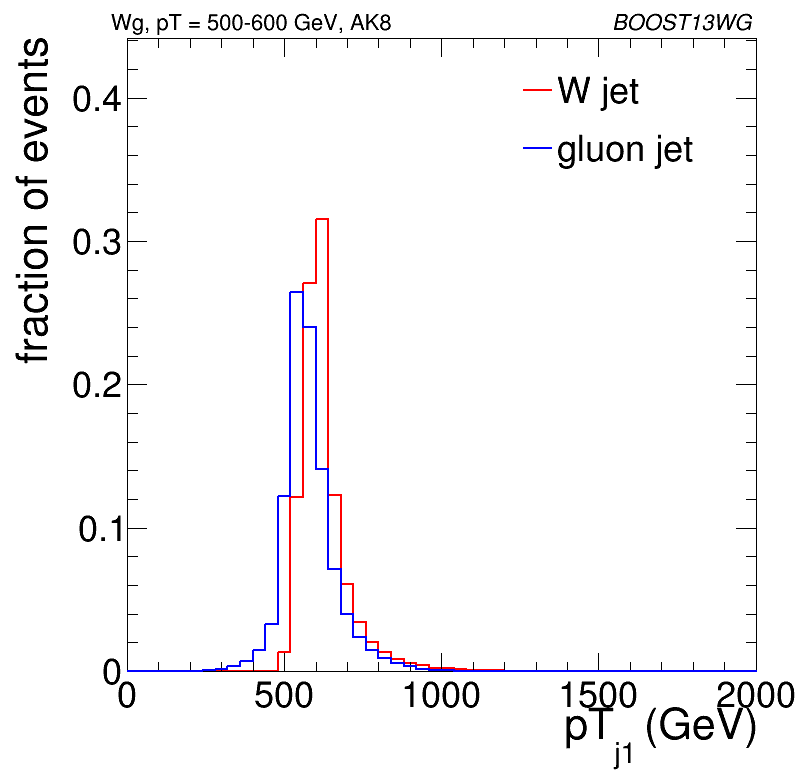
\includegraphics[width=0.30\textwidth]{./Figures/WTagging/pT500/AKtR08/jpt1.png}}
%\subfigure[\antikt R=1.2]{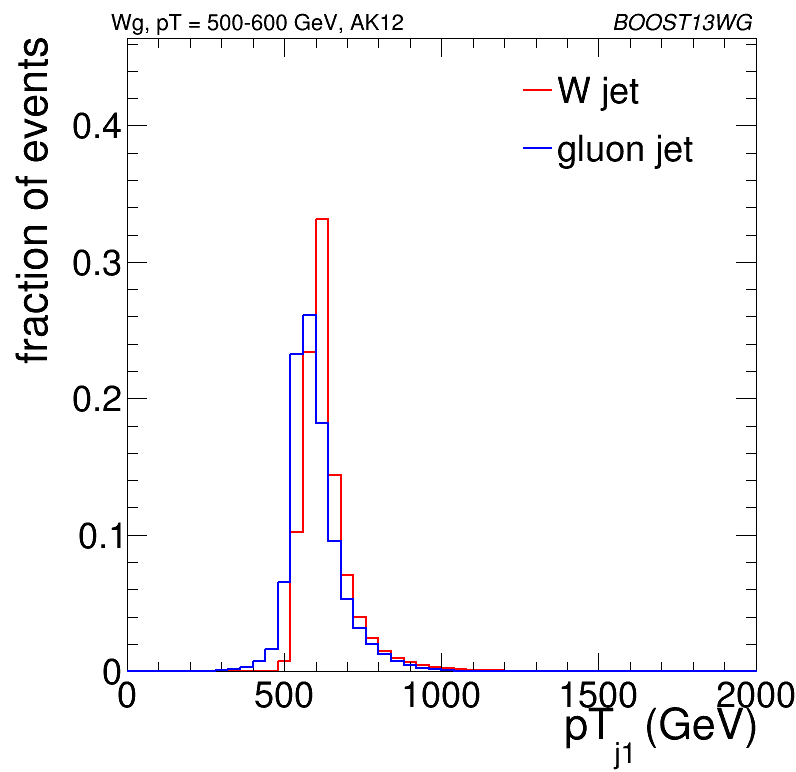
\includegraphics[width=0.30\textwidth]{./Figures/WTagging/pT500/AKtR12/jpt1.png}}
%\caption{Comparisons of the leading jet \pt spectrum of the $gg$
%  background to the $WW$ signal in the \pt 500-600 GeV parton \pt~slice using the
%  different \antikt jet distance parameters explored in this \pt~bin. These
%  distributions are formed prior to the 500-600 GeV leading jet \pt~requirement.} 
%\label{fig:pt500_basics}
%
%\end{figure*}
%
%\begin{figure*}
%\begin{center}
%\subfigure[\antikt R=0.4]{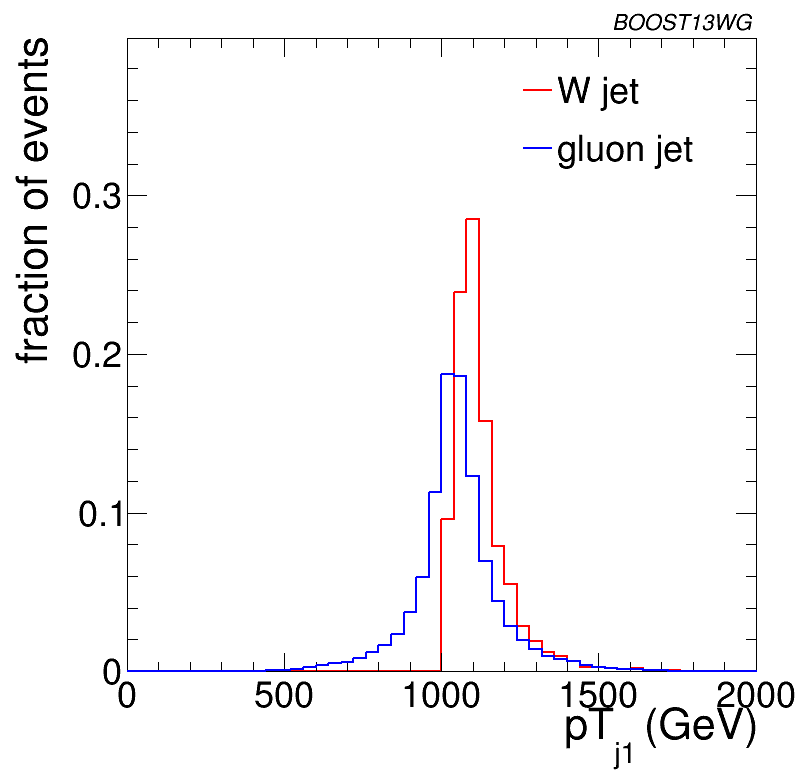
\includegraphics[width=0.30\textwidth]{./Figures/WTagging/pT1000/AKtR04/jpt1.png}}
%\subfigure[\antikt R=0.8]{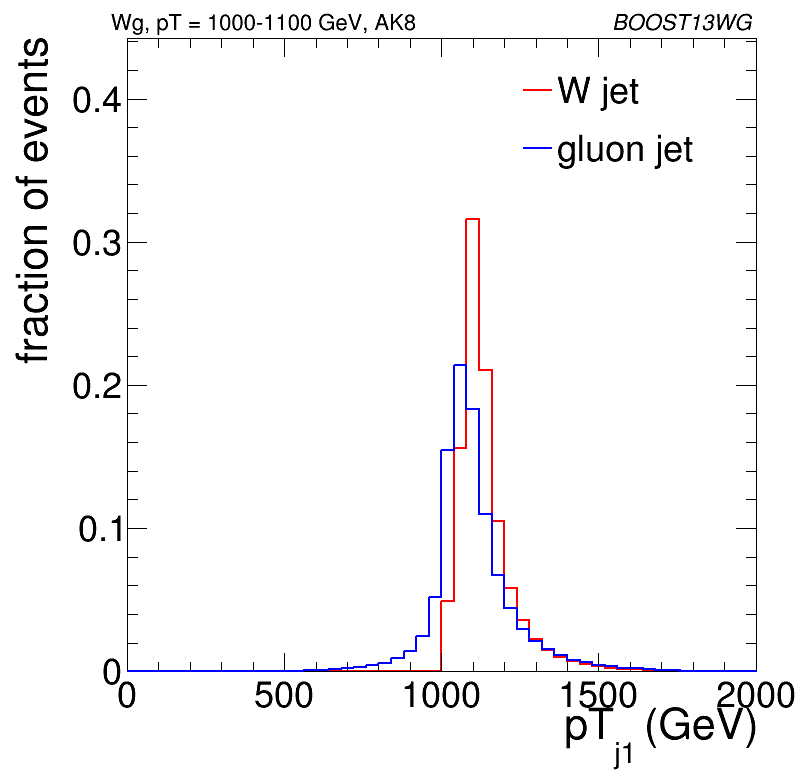
\includegraphics[width=0.30\textwidth]{./Figures/WTagging/pT1000/AKtR08/jpt1.png}}
%\subfigure[\antikt R=1.2]{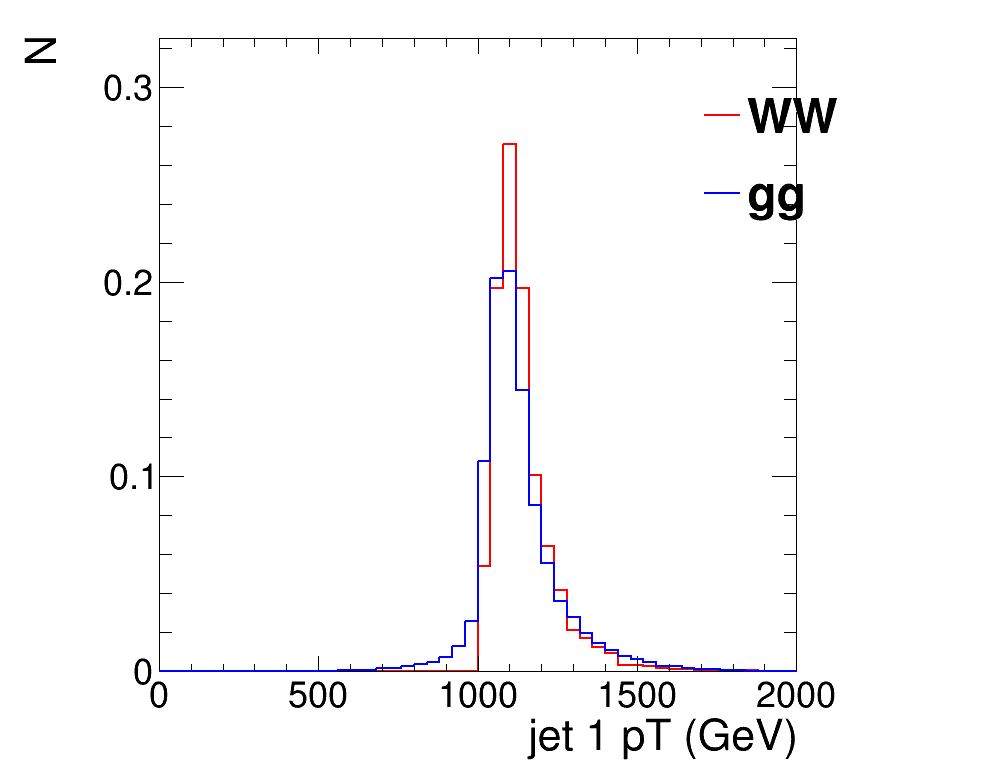
\includegraphics[width=0.30\textwidth]{./Figures/WTagging/pT1000/AKtR12/jpt1.png}}
%\caption{Comparisons of the leading jet \pt spectrum of the $gg$
%  background to the $WW$ signal in the \pt 1.0-1.1 TeV parton \pt~slice using the
%  different \antikt jet distance parameters explored in this \pt~bin. These
%  distributions are formed prior to the 500-600 GeV leading jet \pt~requirement.}
%\label{fig:pt1000_basics}
%
%\end{figure*}

%Figure~\ref{fig:qg_pt500_basics_AKt_R08} shows a comparison of the $\pt$ and $\eta$ distributions of the
% quark and gluon samples with $\pt=500-600$~GeV. 
%\begin{figure*}
%\centering
%\subfigure[Leading jet
%\pT]{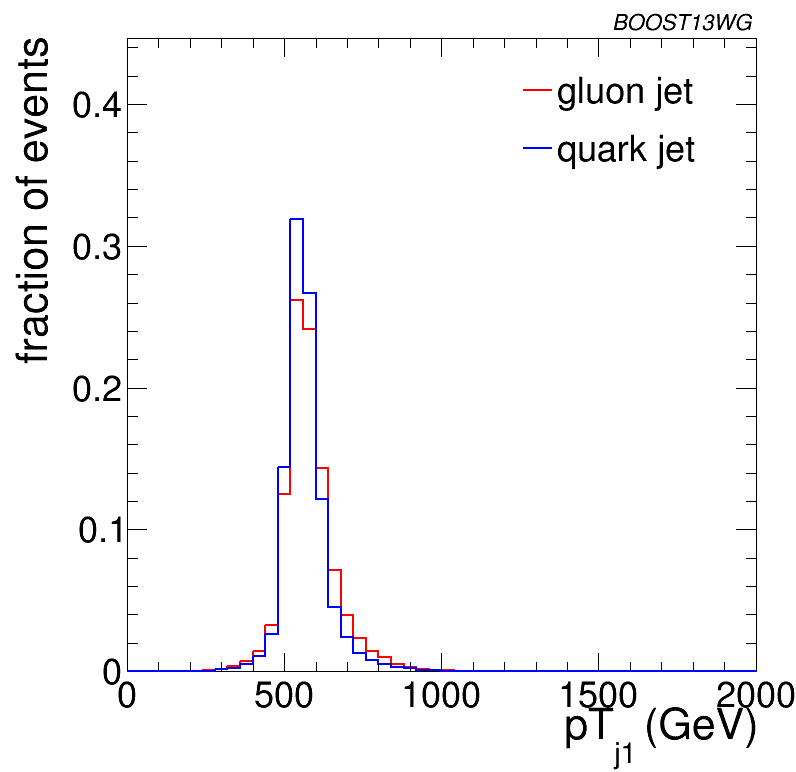
\includegraphics[width=0.40\textwidth]{./Figures/QGTagging/pT500/AKtR08/jpt1.png}}
%\subfigure[Sub-leading jet
%\pT]{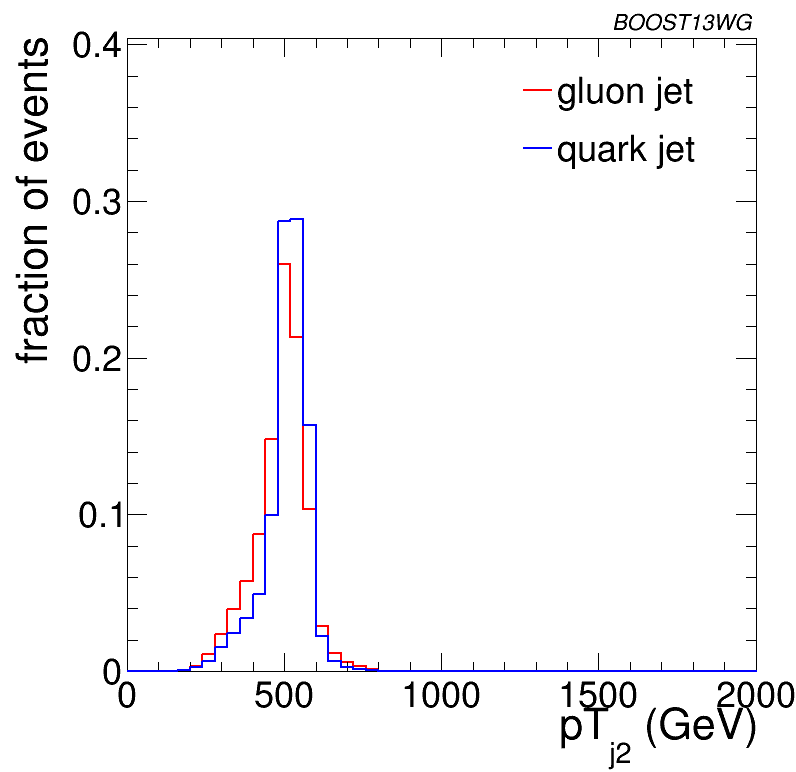
\includegraphics[width=0.40\textwidth]{./Figures/QGTagging/pT500/AKtR08/jpt2.png}}\\
%\subfigure[Leading jet
%$\eta$]{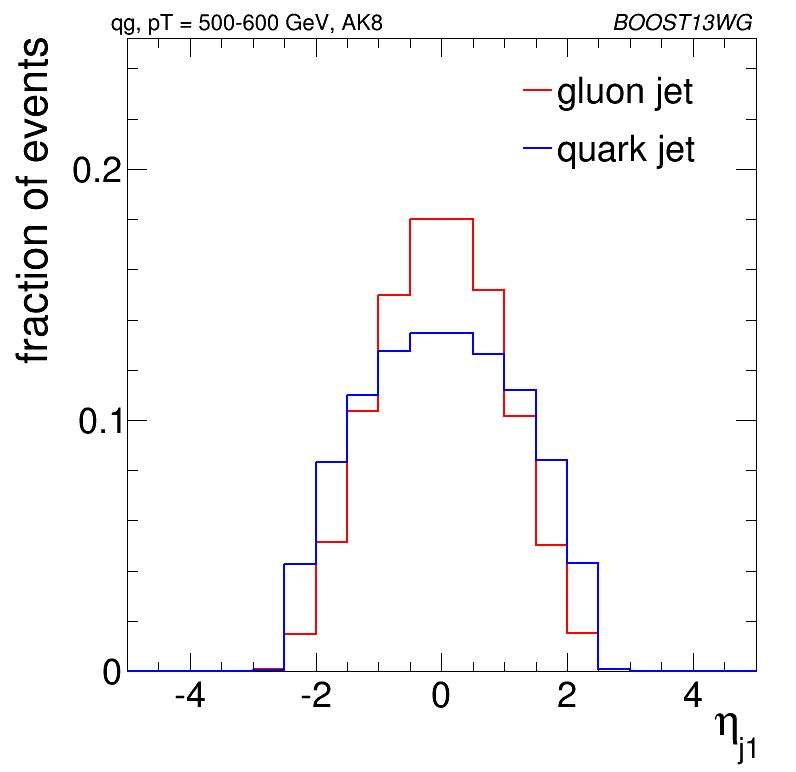
\includegraphics[width=0.40\textwidth]{./Figures/QGTagging/pT500/AKtR08/jeta1.png}}
%\subfigure[Sub-leading jet
%$\eta$]{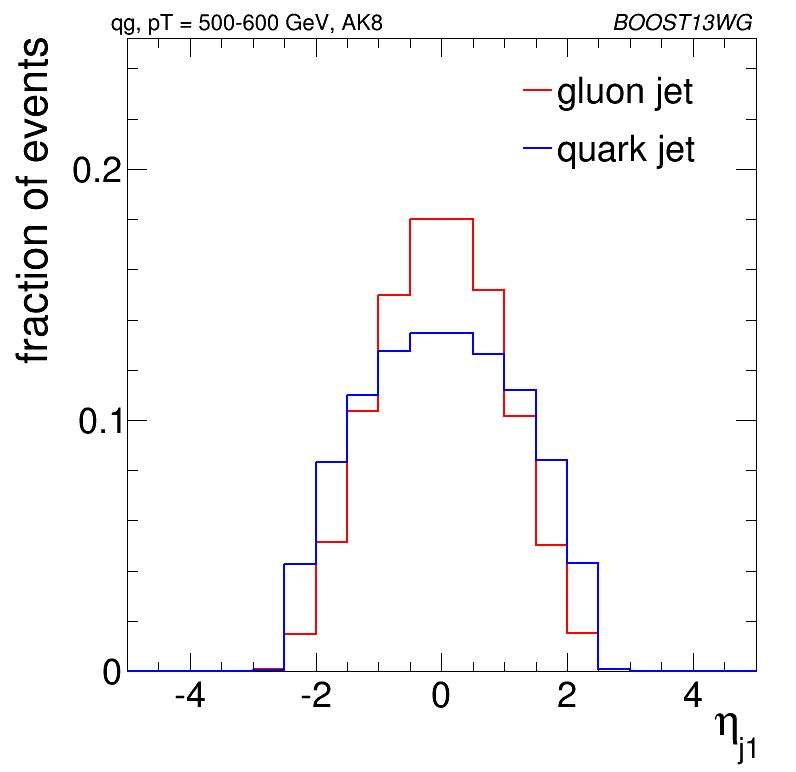
\includegraphics[width=0.40\textwidth]{./Figures/QGTagging/pT500/AKtR08/jeta2.png}}
%\caption{Comparisons of quark and gluon $\pt$ and $\eta$ 
%distributions in the sample used for the jets of $\pt=500-600 \GeV$ bin using the anti-\kT R=0.8 algorithm.}
%\label{fig:qg_pt500_basics_AKt_R08}
%
%\end{figure*}
%%
%The differences in the $\pt$ distributions can be attributed to different out-of-cone radiation
%patterns for quark and gluons; these differences become smaller as the $R$ parameter is increased.
%The different $\eta$ distributions are related to the different
%parton distribution functions initiating $qq$ and $gg$ production. The qualitative features of the 
%$\eta$ distributions do not change as the $R$ parameter is changed. As the $\pt$ increases, 
%the $\eta$ distributions peak more strongly near zero, as the probability peaks for processes
%initiated by partons of comparable energy. In our analysis, we make a narrow window cut of 100 GeV
% in $\pt$ after showering, and so the effects of the different $q/g$ $\pt$ spectra on our analysis
%is suppressed. ({\bf ED: check})

\subsection{Single Variable Discrimination}


Figure~\ref{fig:qg_pt500_mass_AKt_R08} shows the mass of jets in the quark and gluon samples when using
different groomers, and the ungroomed jet mass, for jets with
R=0.8 and in the $\pt=500-600 \GeV$ bin. 
\begin{figure*}
\centering
\subfigure[Ungroomed mass]{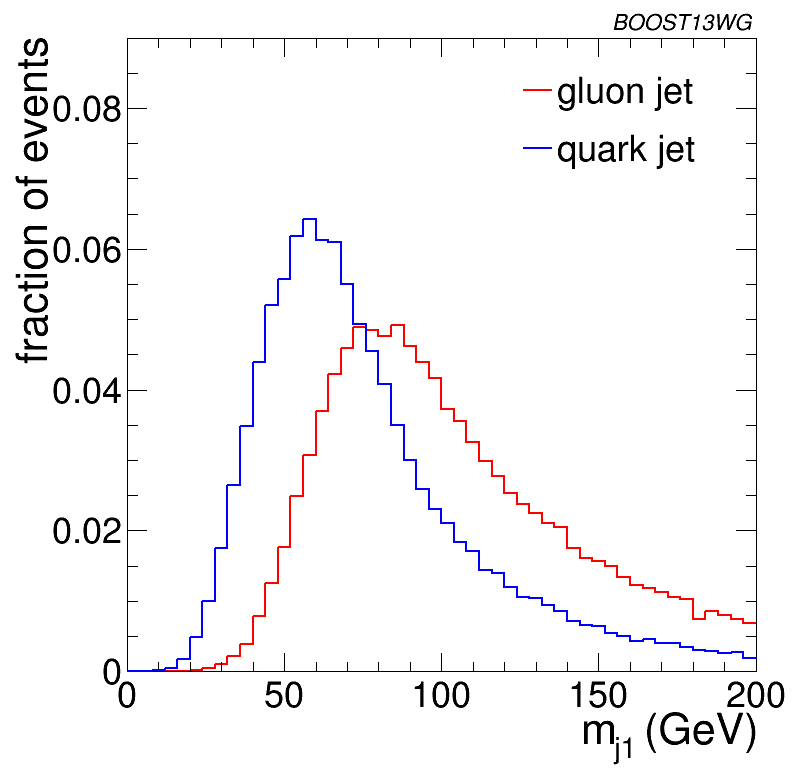
\includegraphics[width=0.30\textwidth]{./Figures/QGTagging/pT500/AKtR08/jmass1.png}}
\subfigure[Pruned mass]{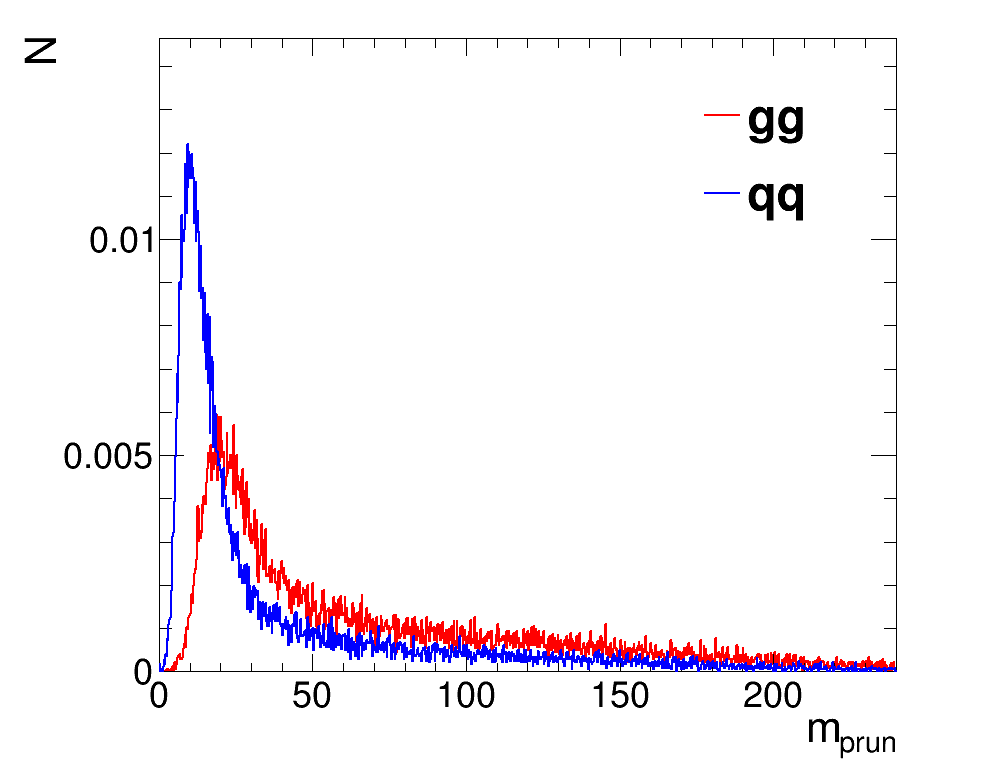
\includegraphics[width=0.30\textwidth]{./Figures/QGTagging/pT500/AKtR08/h_mass_prun.png}}
\subfigure[Trimmed mass]{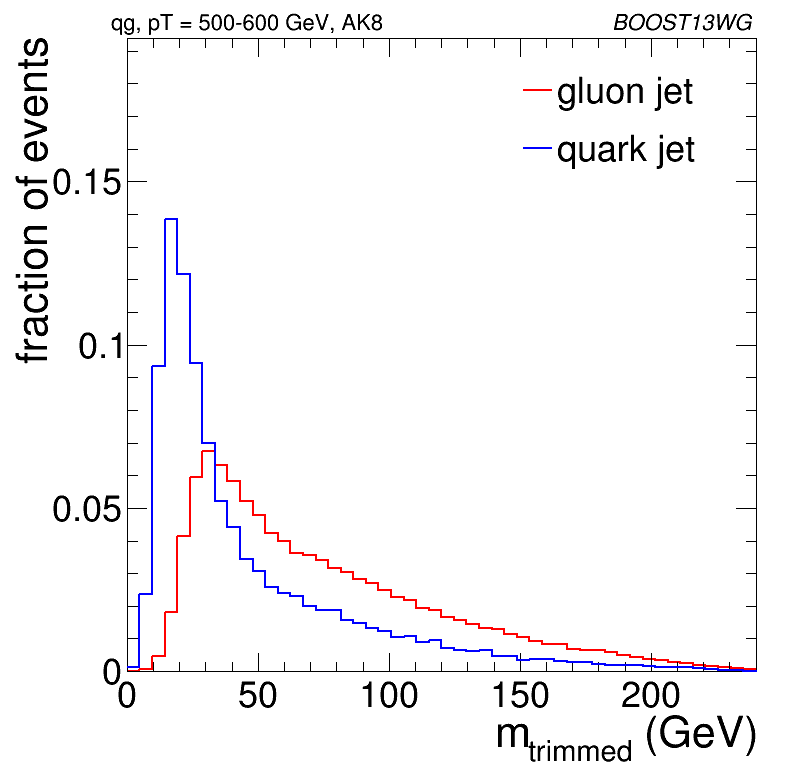
\includegraphics[width=0.30\textwidth]{./Figures/QGTagging/pT500/AKtR08/h_mass_trim.png}}\\
\subfigure[mMDT mass]{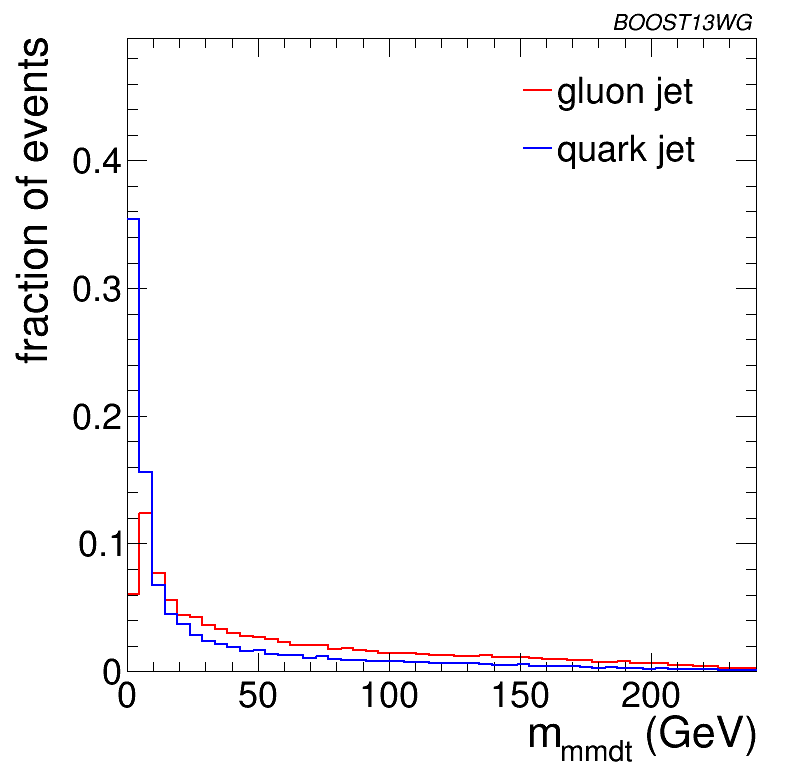
\includegraphics[width=0.30\textwidth]{./Figures/QGTagging/pT500/AKtR08/h_mass_mmdt.png}}
\subfigure[Soft-drop $\beta=2$ mass]{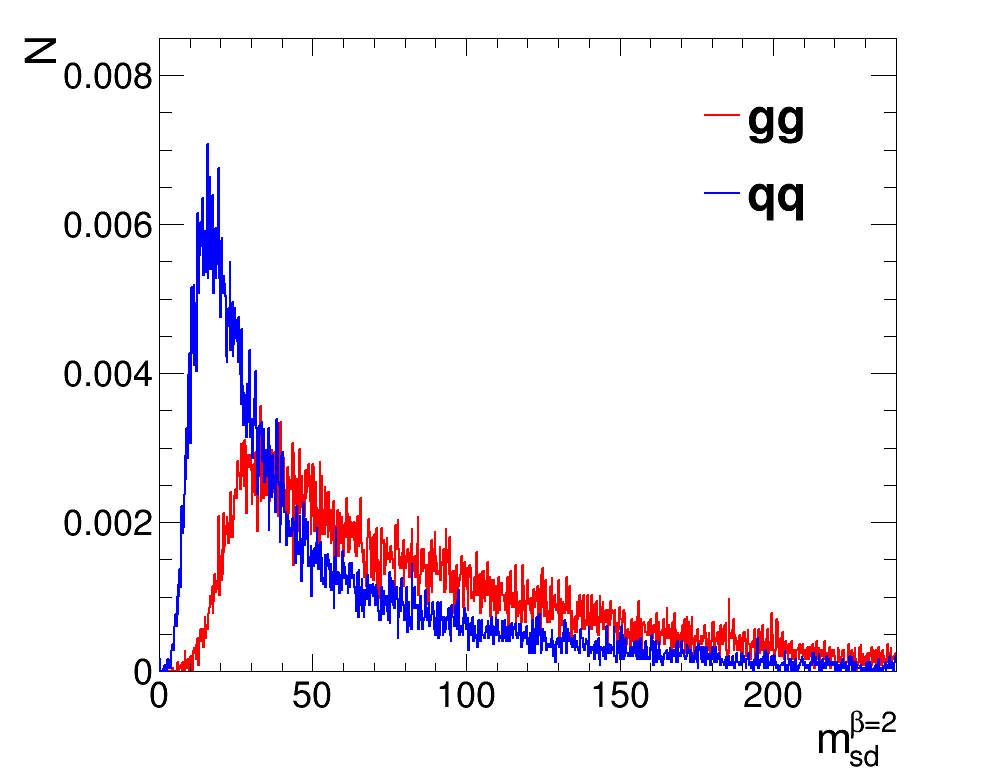
\includegraphics[width=0.30\textwidth]{./Figures/QGTagging/pT500/AKtR08/h_mass_sdb2.png}}
\subfigure[Soft-drop $\beta=-1$ mass]{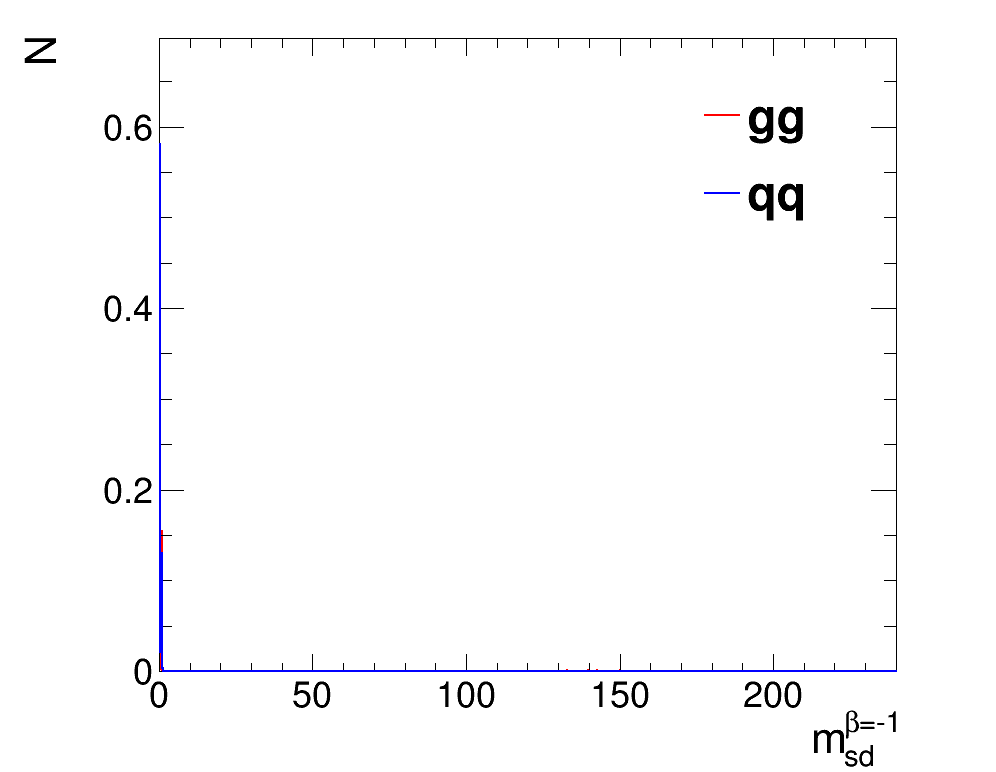
\includegraphics[width=0.30\textwidth]{./Figures/QGTagging/pT500/AKtR08/h_mass_sdm1.png}}
\caption{Comparisons of ungroomed and groomed quark and gluon mass distributions for leading jets in the 
$\pt=500-600 \GeV$ bin using the anti-\kT R=0.8 algorithm. }
\label{fig:qg_pt500_mass_AKt_R08}
\end{figure*}
Qualitatively, the application of grooming shifts the mass distributions towards
lower values when compared to the ungroomed mass, as expected. No clear gain in discrimination can be seen, and for
certain grooming parameters, such as the use of soft drop with $\beta=-1$ a clear
loss in discrimination power is observed; this is because the soft-drop condition for $\beta=-1$ discards collinear radiation, and the differences between quarks and gluons are manifest in the collinear structure (spin, splitting functions, etc.). 


\begin{figure*}
\centering
\subfigure[$C_1^{\beta=0}$]{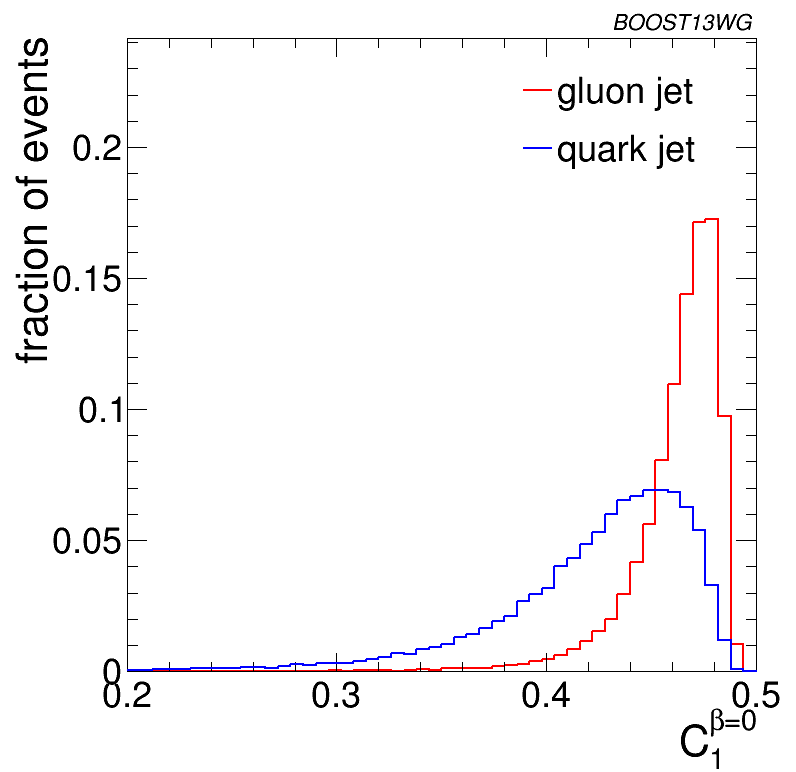
\includegraphics[width=0.30\textwidth]{./Figures/QGTagging/pT500/AKtR08/h_c1_b0.png}}
\subfigure[$C_1^{\beta=1}$]{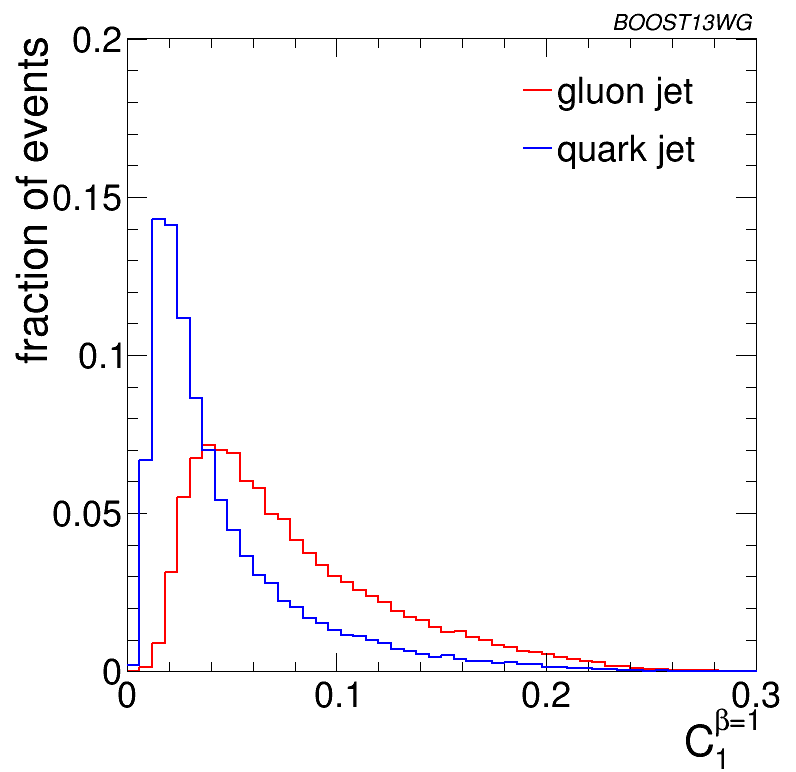
\includegraphics[width=0.30\textwidth]{./Figures/QGTagging/pT500/AKtR08/h_c1_b1.png}}
\subfigure[$C_1^{\beta=2}$]{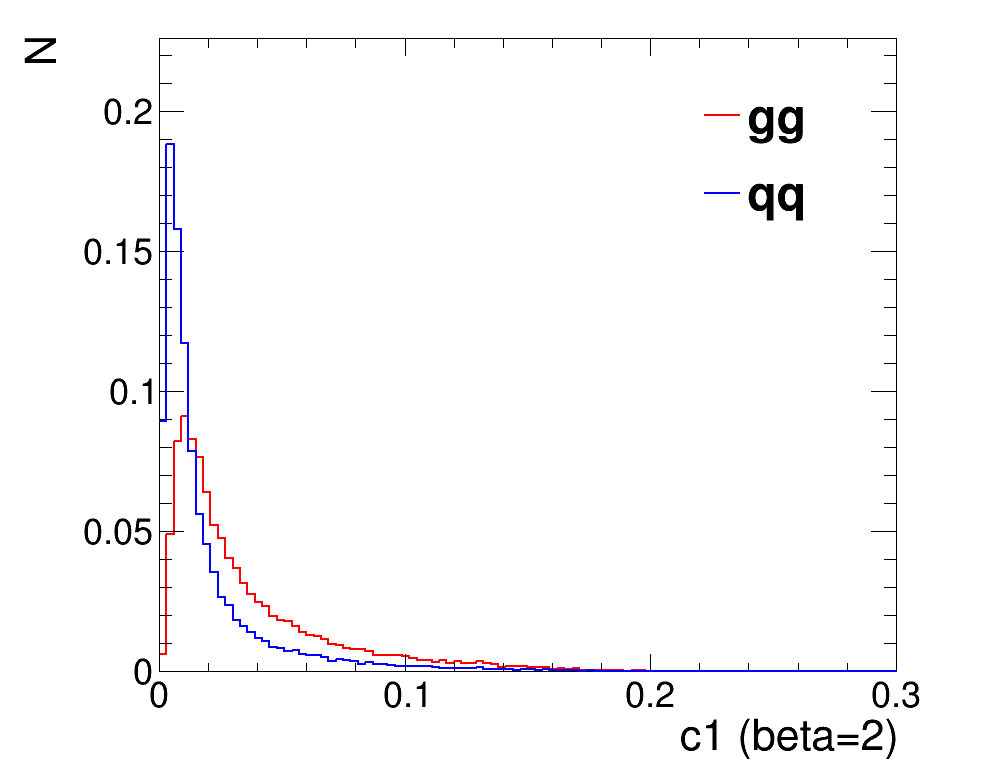
\includegraphics[width=0.30\textwidth]{./Figures/QGTagging/pT500/AKtR08/h_c1_b2.png}}\\
\subfigure[$\Gamma_{Qjet}$]{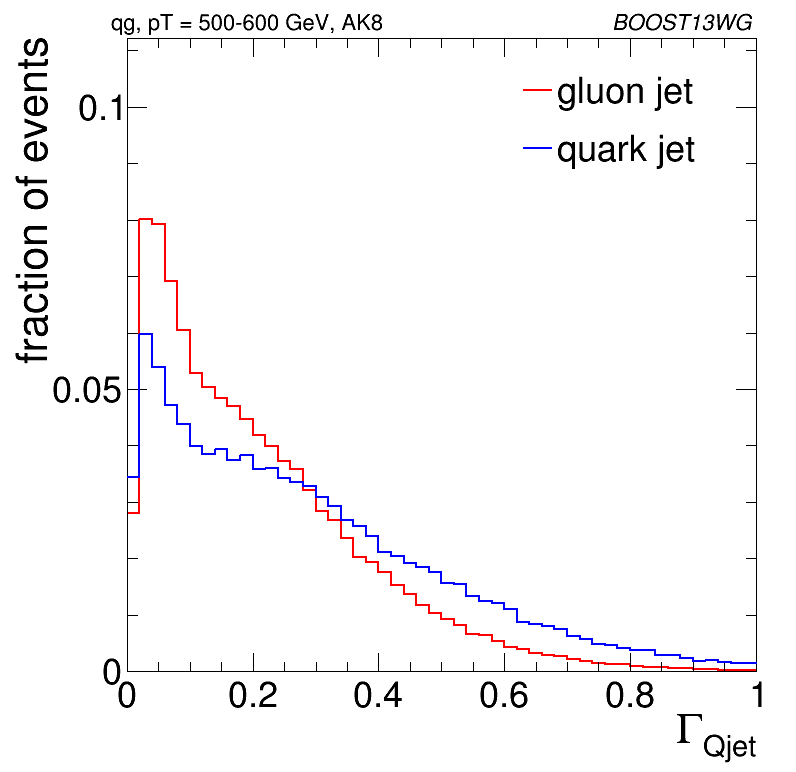
\includegraphics[width=0.30\textwidth]{./Figures/QGTagging/pT500/AKtR08/h_qjetVol.png}}
\subfigure[$\rm{n_ {constits}}$]{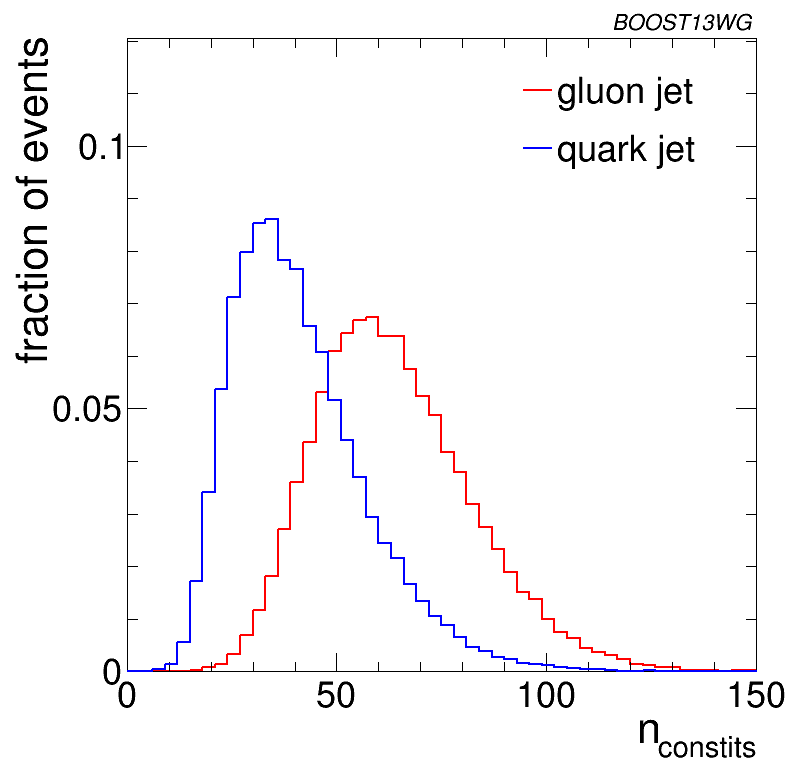
\includegraphics[width=0.30\textwidth]{./Figures/QGTagging/pT500/AKtR08/h_multiplicity.png}}
\subfigure[$\tau_{1}^{\beta=1}$]{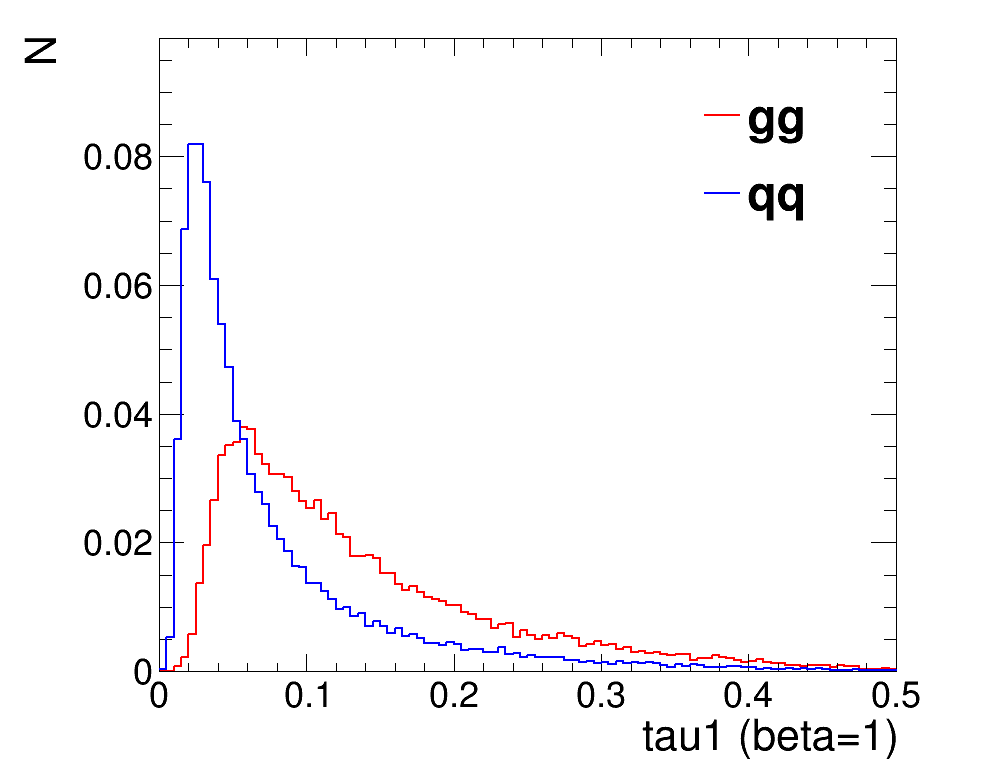
\includegraphics[width=0.30\textwidth]{./Figures/QGTagging/pT500/AKtR08/h_tau1_b1.png}}\\
\subfigure[$\tau_{1}^{\beta=2}$]{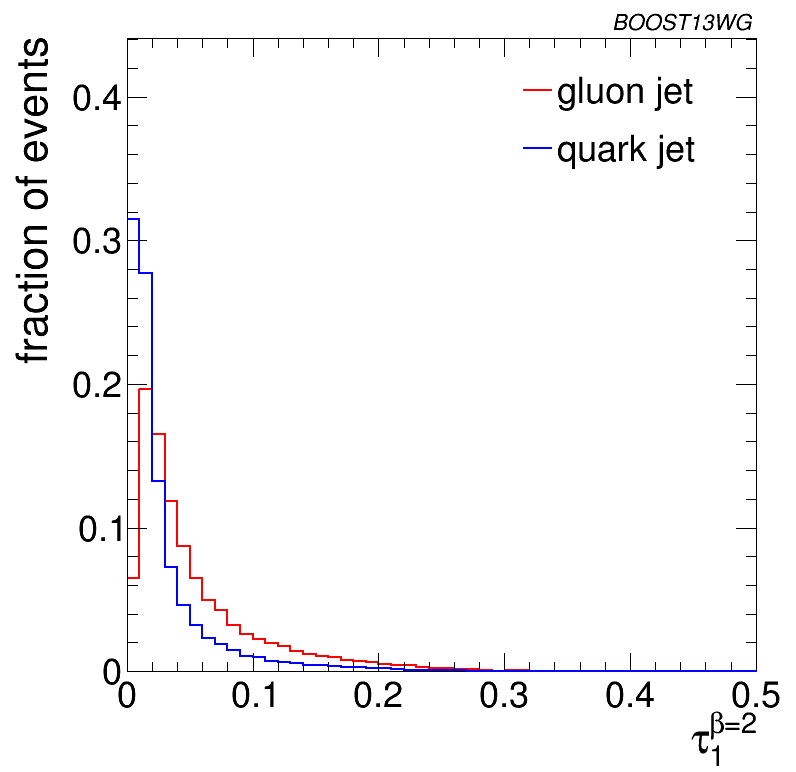
\includegraphics[width=0.30\textwidth]{./Figures/QGTagging/pT500/AKtR08/h_tau1_b2.png}}
\caption{Comparisons of quark and gluon distributions of different substructure variables for leading jets in the 
$\pt=500-600 \GeV$ bin using the anti-\kT R=0.8 algorithm. }
\label{fig:qg_pt500_subst_AKt_R08}
\end{figure*}

The quark and gluon distributions of different substructure variables
are shown in Figure~\ref{fig:qg_pt500_subst_AKt_R08}. Among those
considered, one can see by eye that $n_{\rm constits}$ provides the highest separation
power, followed by $C_1^{\beta=0}$ and $C_1^{\beta=1}$, as was also
found by the CMS and ATLAS Collaborations\refneeded. 

To more quantitatively study the power of each observable as a
discriminator for quark/gluon tagging, ROC curves are built by scanning each distribution
and plotting the background efficiency (to select gluon jets) vs.~the signal efficiency (to select quark jets). 
Figure~\ref{fig:qg_pt300_single} shows these ROC curves for all of the
substructure variables shown in 
Figure~\ref{fig:qg_pt500_subst_AKt_R08}, along with the ungroomed mass, representing the 
best performing mass variable, for R=0.4, 0.8 and 1.2 jets in the $\pt=300-400\GeV$
bin. In addition, the ROC curve for a tagger built from a BDT
combination of all the variables (see Section~\ref{sec:multivariate}) is shown.
%
\begin{figure*}
\centering
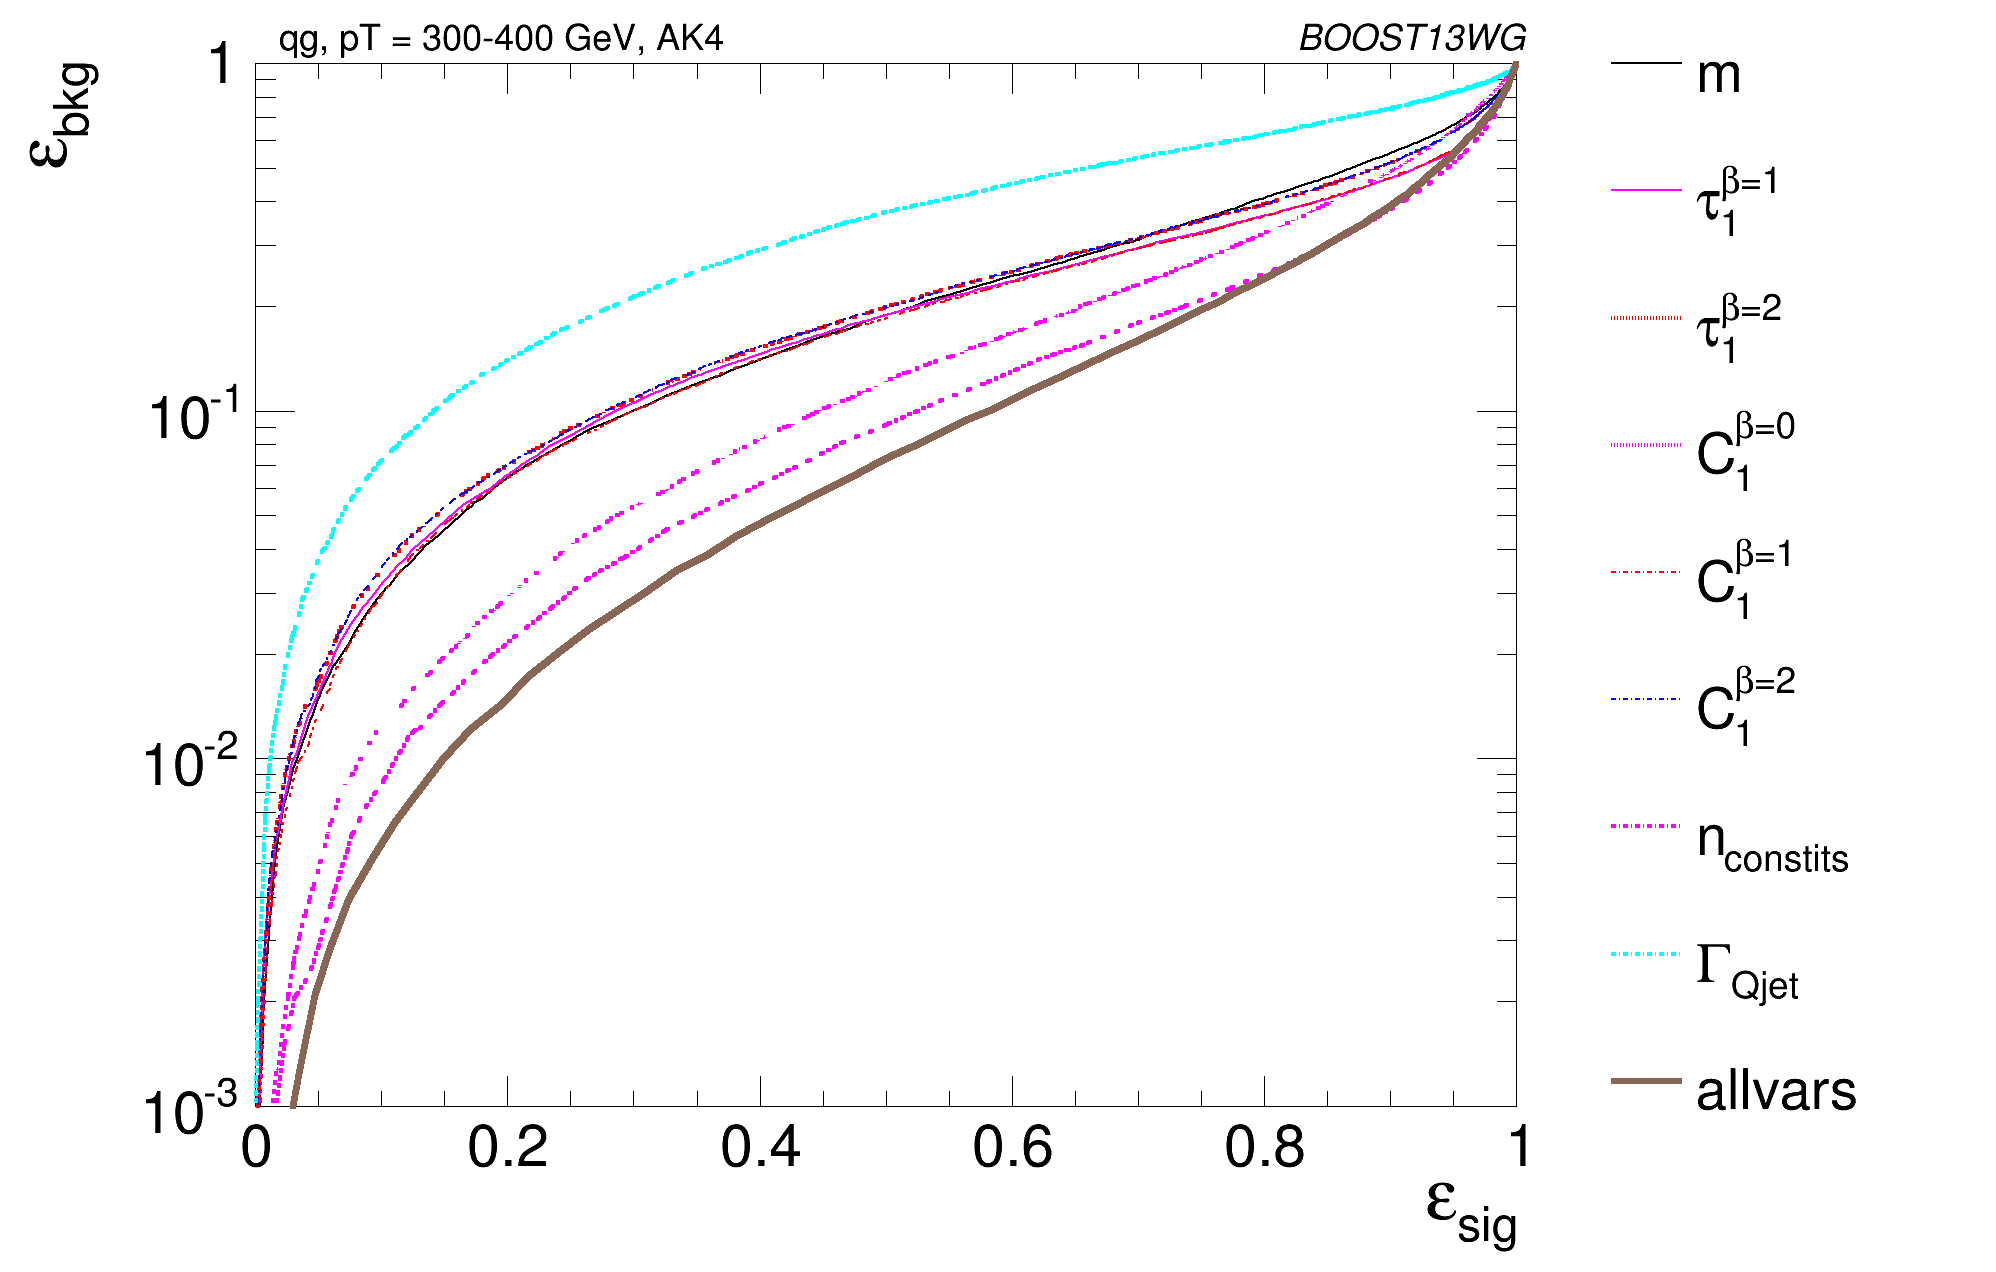
\includegraphics[width=0.48\textwidth]{./Figures/QGTagging/pT300/AKtR04/Rocs_1D_single.png}
%\includegraphics[width=0.4\textwidth]{./Figures/QGTagging/pT1000/AKtR04/Rocs_1D_single.png}\\
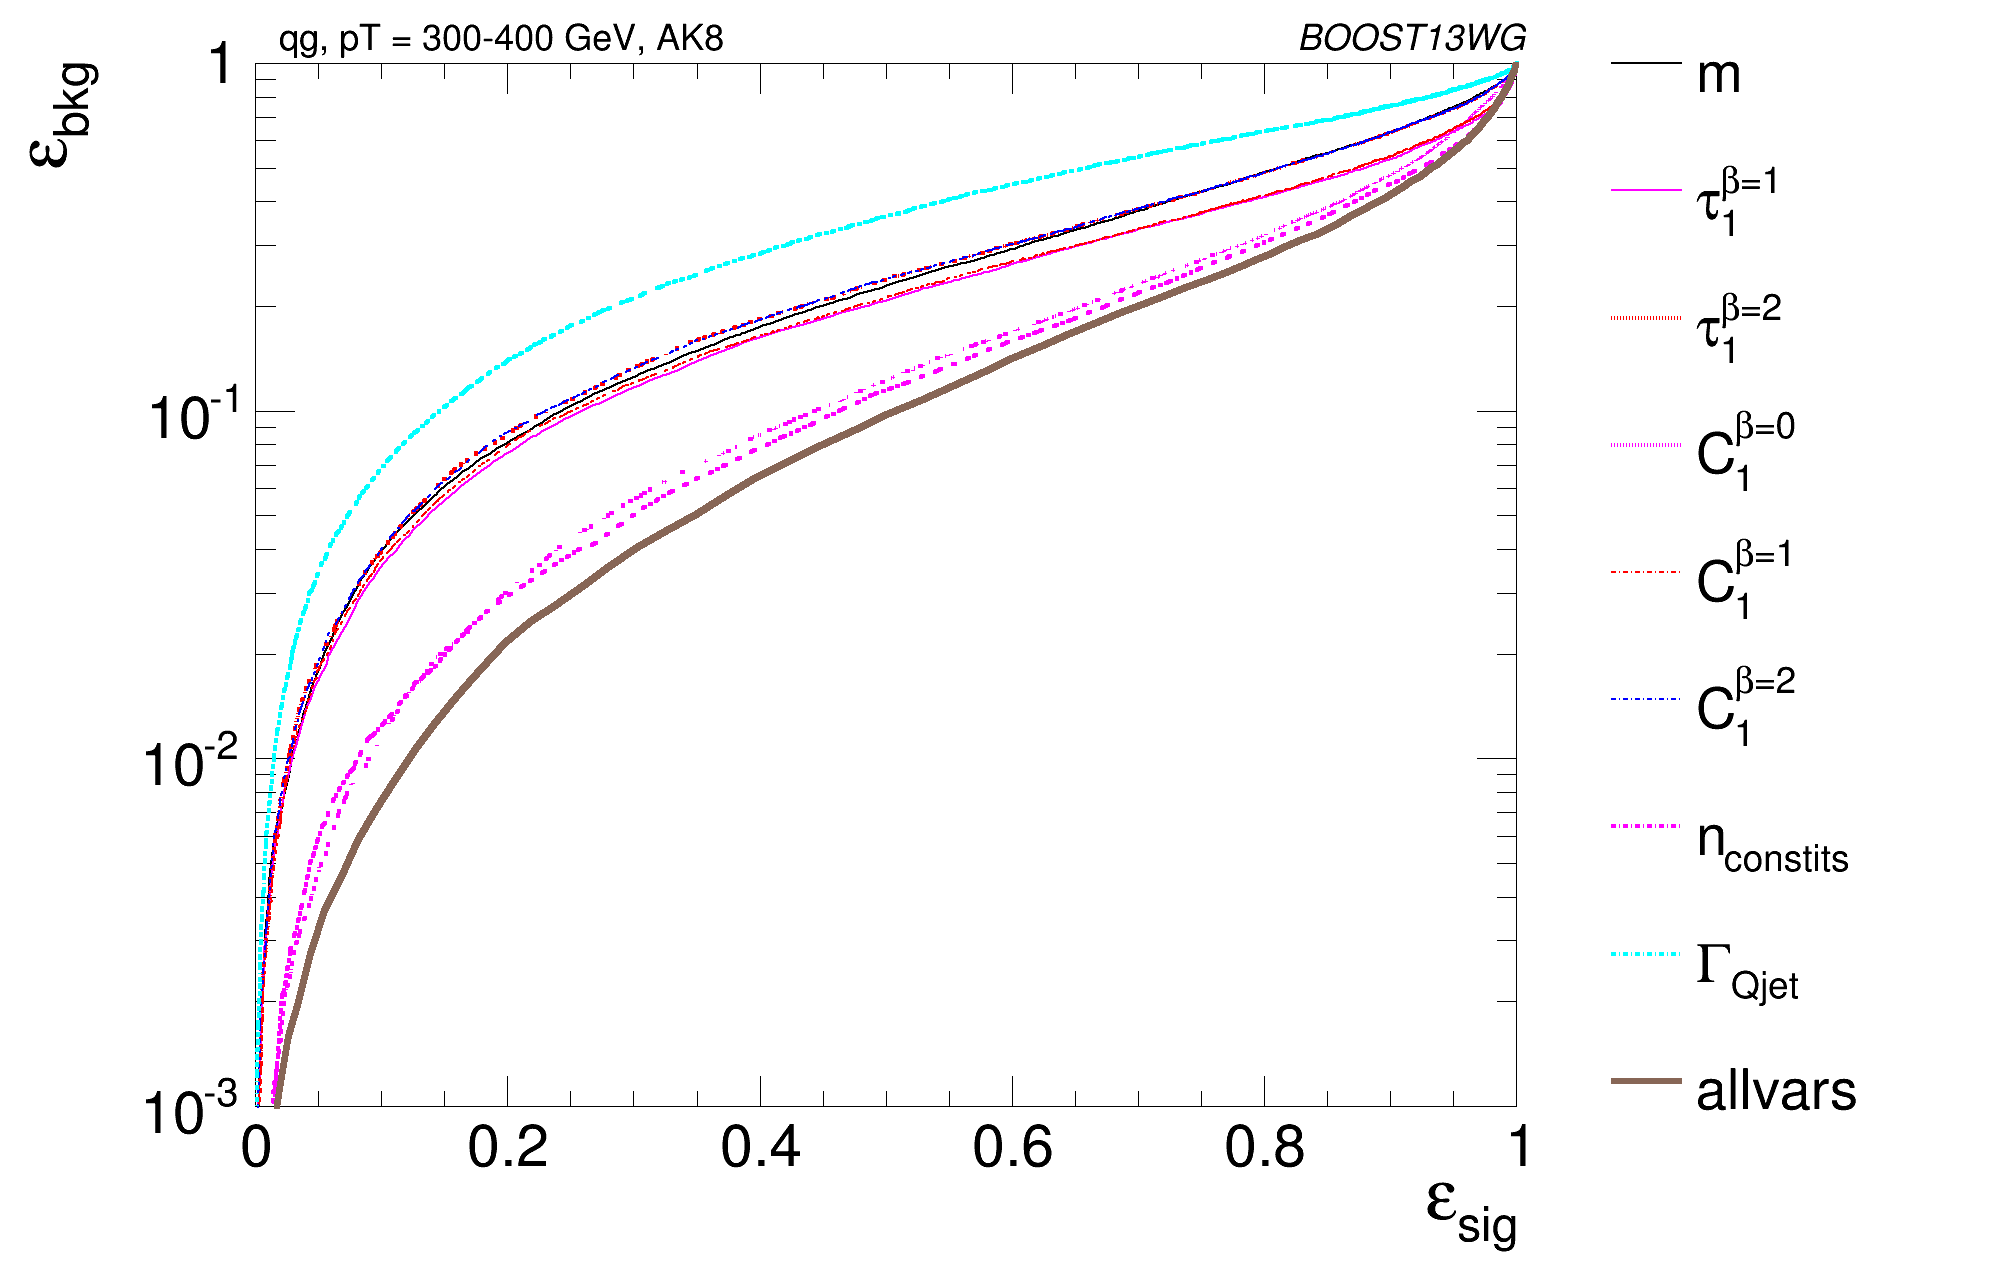
\includegraphics[width=0.48\textwidth]{./Figures/QGTagging/pT300/AKtR08/Rocs_1D_single.png}
%\includegraphics[width=0.4\textwidth]{./Figures/QGTagging/pT1000/AKtR08/Rocs_1D_single.png}\\
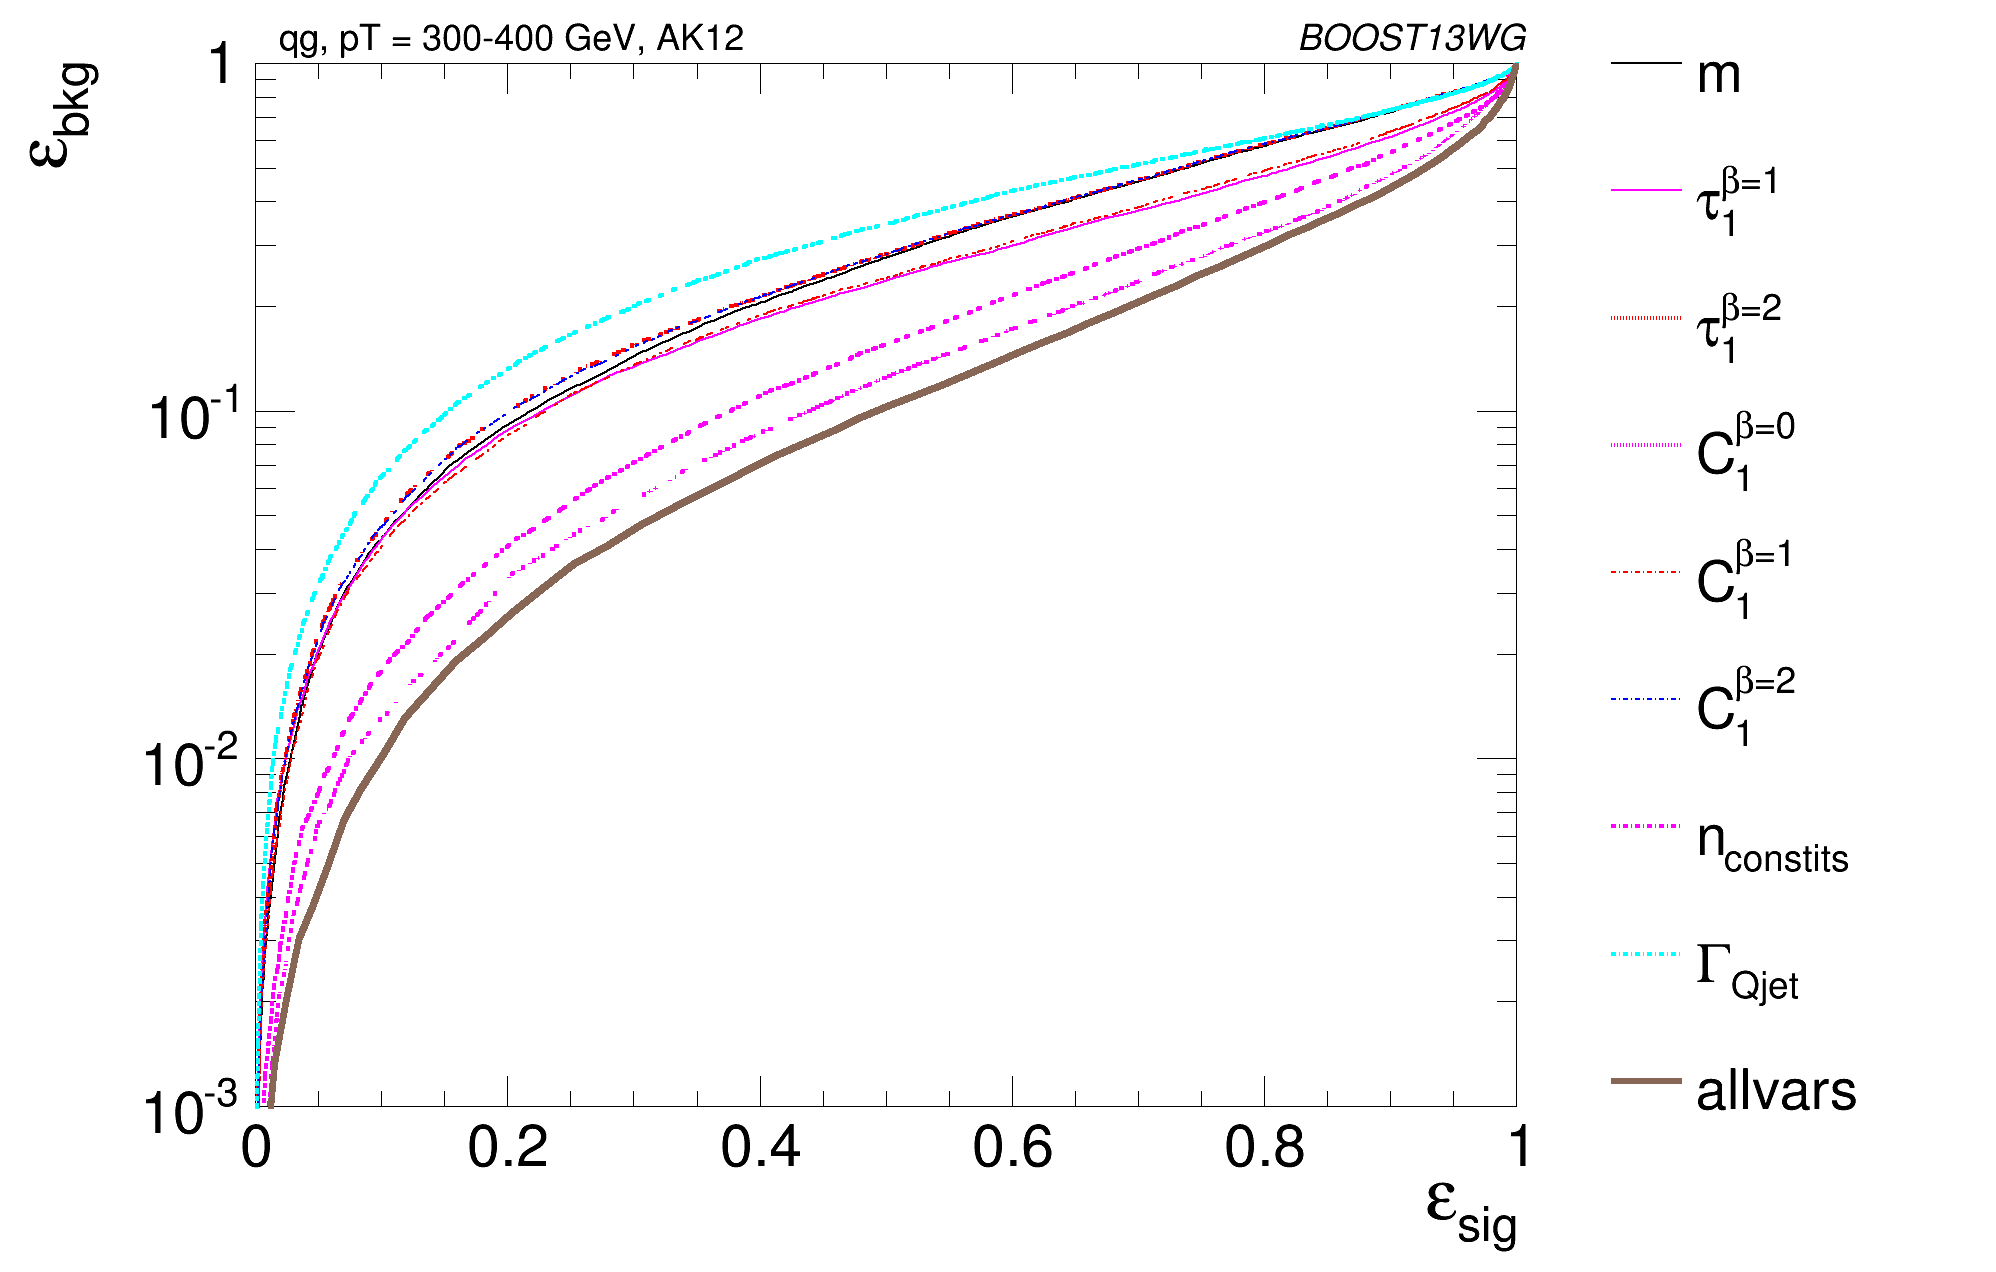
\includegraphics[width=0.48\textwidth]{./Figures/QGTagging/pT300/AKtR12/Rocs_1D_single.png}
%\includegraphics[width=0.4\textwidth]{./Figures/QGTagging/pT1000/AKtR12/Rocs_1D_single.png}\\
\caption{The ROC curve for all single variables considered for
  quark-gluon discrimination in the \pt 300-400 GeV bin using the
  anti-\kT R=0.4, 0.8 and 1.2 algorithm.{\bf ED: Hard to tell the lines on the
    plots apart}}
\label{fig:qg_pt300_single}
\end{figure*}
%
Clearly, $n_{\rm constits}$ is the best performing variable for all Rs, even though $C_1^{\beta=0}$ is close, particularly
for R=0.8. Most other variables have similar performance, except $\Gamma_{\rm Qjet}$, which shows significantly worse
discrimination (this may be due to our choice of
rigidity $\alpha = 0.1$, with other studies suggesting that a smaller value,
such as $\alpha = 0.01$, produces better results\refneeded). The combination of all variables shows somewhat better discrimination.

We now examine how performance of masses and substructure observables changes with $\pt$ and $R$. For jet masses, few variations are observed as the 
radius parameter of the jet reconstruction is increased in the two highest $\pt$ bins; this is because the radiation
is more collimated and the dependence on $R$ is consequently smaller.
However, for the $300-400\GeV$ bin, the use of small-$R$ jets produces a shift in the
mass distributions towards lower values, so that large-$R$ jet masses are more stable
with $\pt$ and small-$R$ jet masses are smaller at low-$\pt$ as expected from the spatial
constraints imposed by the $R$ parameter. These statements are explored more 
quantitatively later in this section. ({\bf BS: Do we have plots for this?})

The evolution of some of the substructure variable distributions with $\pt$ and R is less trivial than
 for the jet masses. In particular, changing the $R$ parameter at high $\pt$ changes significantly the $C_a^{\beta}$
for $\beta>0$ and the $n_{\rm constits}$ distributions, while leaving all other distributions qualitatively unchanged. 
This is illustrated in Figure~\ref{fig:Rdep_qg_C_pt1000} for $\beta=0$ and $\beta=1$ using $a=1$ in both cases for
jets with $\pt=1.0-1.1\TeV$. 

 %
\begin{figure*}
\centering
\subfigure[$C_1^{\beta=0}$, $R=0.4$]{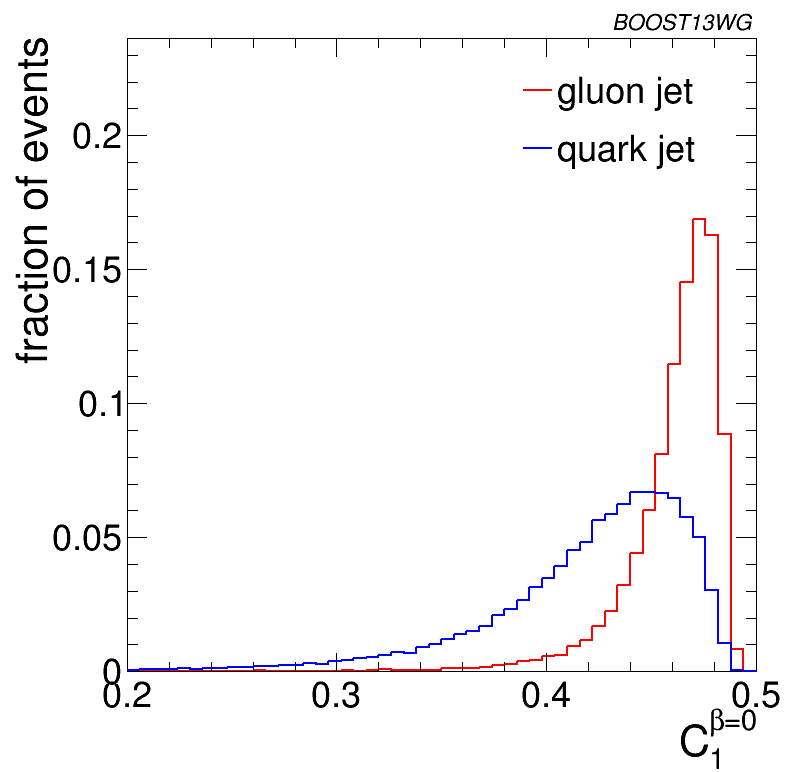
\includegraphics[width=0.30\textwidth]{./Figures/QGTagging/pT1000/AKtR04/h_c1_b0.png}}
\subfigure[$C_1^{\beta=0}$, $R=0.8$]{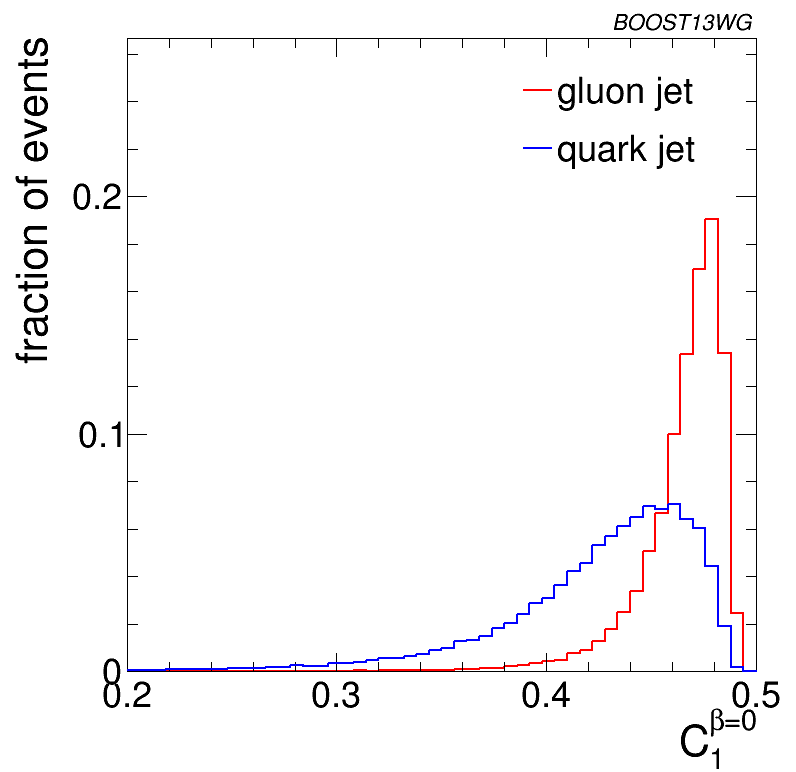
\includegraphics[width=0.30\textwidth]{./Figures/QGTagging/pT1000/AKtR08/h_c1_b0.png}}
\subfigure[$C_1^{\beta=0}$, $R=1.2$]{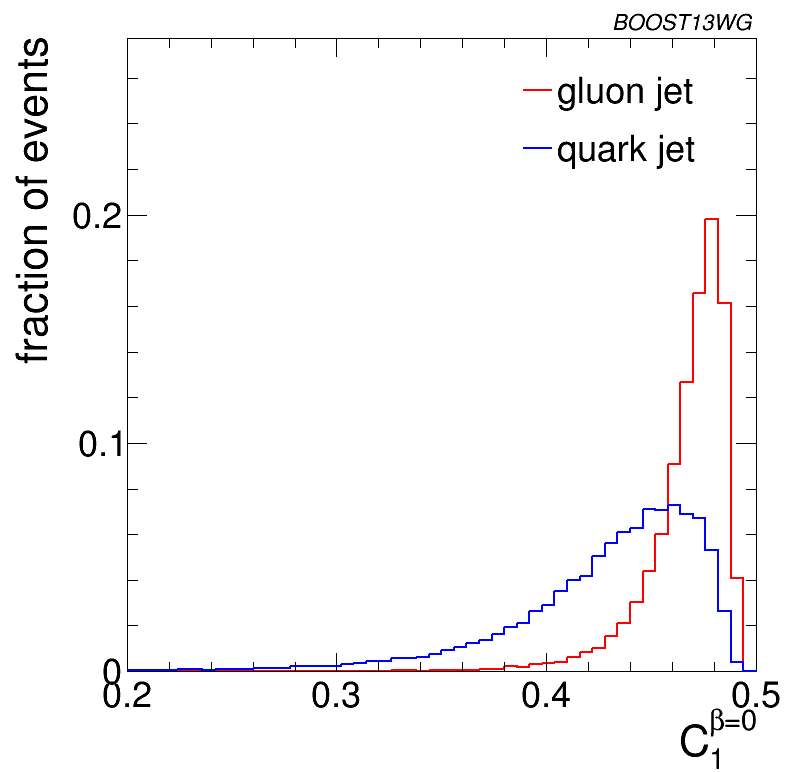
\includegraphics[width=0.30\textwidth]{./Figures/QGTagging/pT1000/AKtR12/h_c1_b0.png}}\\
\subfigure[$C_1^{\beta=1}$, $R=0.4$]{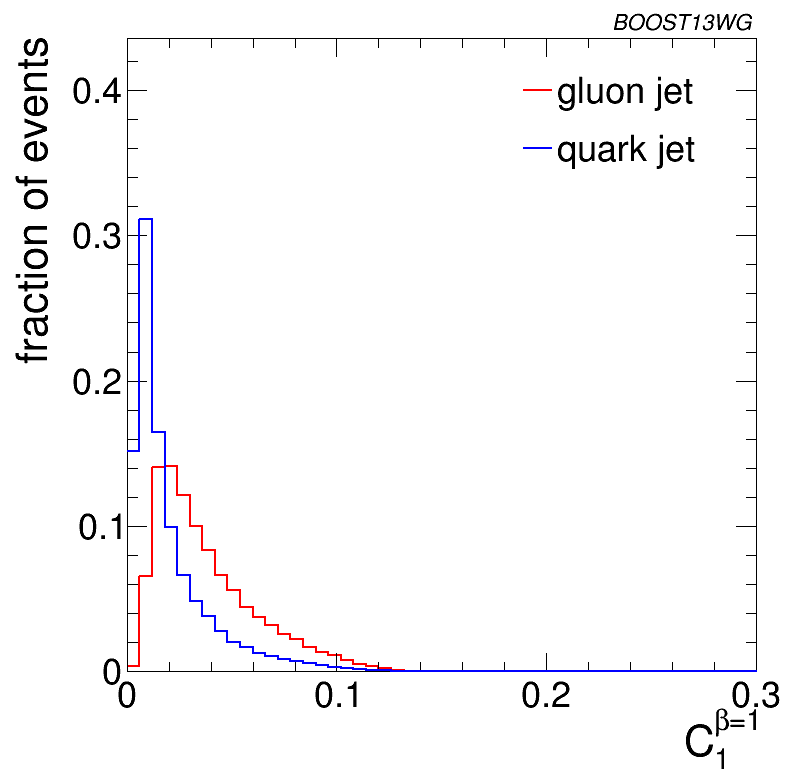
\includegraphics[width=0.30\textwidth]{./Figures/QGTagging/pT1000/AKtR04/h_c1_b1.png}}
\subfigure[$C_1^{\beta=1}$, $R=0.8$]{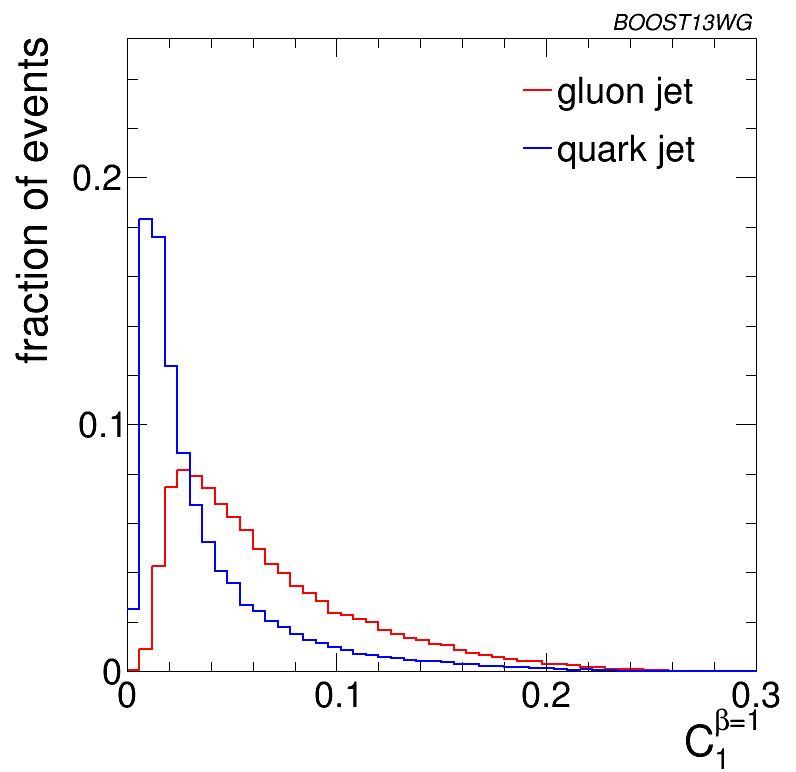
\includegraphics[width=0.30\textwidth]{./Figures/QGTagging/pT1000/AKtR08/h_c1_b1.png}}
\subfigure[$C_1^{\beta=1}$, $R=1.2$]{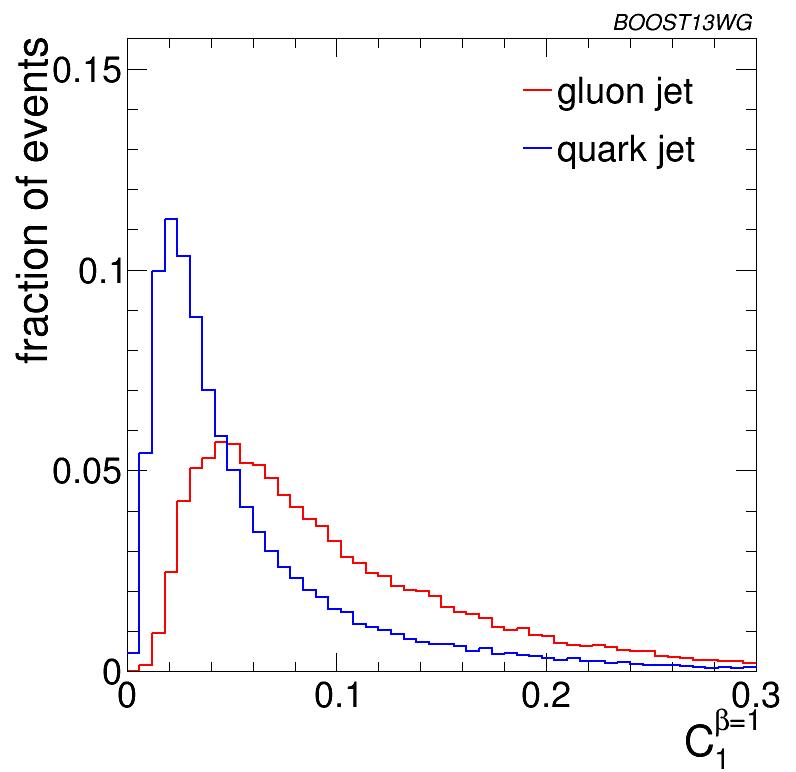
\includegraphics[width=0.30\textwidth]{./Figures/QGTagging/pT1000/AKtR12/h_c1_b1.png}}\\
\caption{Comparisons of quark and gluon distributions of $C_1^{\beta=0}$ (top) and $C_1^{\beta=1}$ (bottom) 
for leading jets in the $\pt=1-1.1 \TeV$ bin using the anti-\kT algorithm with $R=0.4$, 0.8 and 1.2. }
\label{fig:Rdep_qg_C_pt1000}
\end{figure*}
The shift towards lower values with changing R is evident for the $C_1^{\beta=1}$ distributions, while the stability
of $C_1^{\beta=0}$ can also be observed. These features are present in all $\pt$ bins studied, but are even more
pronounced for lower $\pt$ bins. The shape of the Q-jet volatility distribution shows some non-trivial shape that
deserves some explanation. Two peaks are observed, one at low volatility values and one at mid-volatility. These
peaks are generated by two somewhat distinct populations. The high volatility peak arises from jets that get their
mass primarily from soft (and sometimes wide-angle) emissions. The removal of some of the constituents when
building Q-jets thus changes the mass significantly, increasing the volatility. The lower volatility peak corresponds
to jets for which mass is generated by a hard emission, which makes the fraction of Q-jets that change 
the mass significantly to be smaller. Since the probability of a hard emission is proportional to the colour
charge (squared),  the volatility peak is higher for gluon jets by about the colour factor $C_A/C_F$. 



In summary, the overall discriminating power between quarks and gluons
 decreases with increasing R due to the reduction in the amount of out-of-cone radiation differences and 
 and increased contamination from the underlying event ({\bf BS: is this ok?}). The broad performance features discussed for this $\pt$ bin also apply to the higher
$\pt$ bins. These  is further quantified in the next section. 


\subsection{Combined Performance and Correlations}\label{sec:qg_combi}
The quark/gluon tagging performance can be further improved over cuts on single observables by 
combining multiple observables in a BDT; due to the challenging nature of $q$/$g$-tagging, any
improvement in performance with multivariable techniques could be critical for certain analyses, and the 
improvement could be more substantial in data than the marginal benefit found in MC  and shown
in Fig.~\ref{fig:qg_pt300_single}.
 Furthermore, insight can be gained into the 
features allowing for quark/gluon discrimination if the origin of the improvement  is
understood. To quantitatively study this improvement, we build quark/gluon taggers from
every pair-wise combination of variables studied in the previous section for comparison
with the all-variable combination. 

In order to quantitatively study the value of each variable for quark/gluon tagging, we study the gluon 
rejection, defined as $1/\epsilon_{\rm gluon}$, at a fixed quark selection efficiency
of 50\% using jets with $\pt=1-1.1 \TeV$ and for different $R$ parameters. Figure~\ref{fig:qg_pt1000_comb} shows the gluon rejection for each pair-wise combination. 
The pair-wise gluon rejection at 50\% quark efficiency can be compared to the single-variable
values shown along the diagonal. The gluon rejection for the 
BDT all-variable combination is also shown on the bottom right of each plot.
\begin{figure*}
\centering
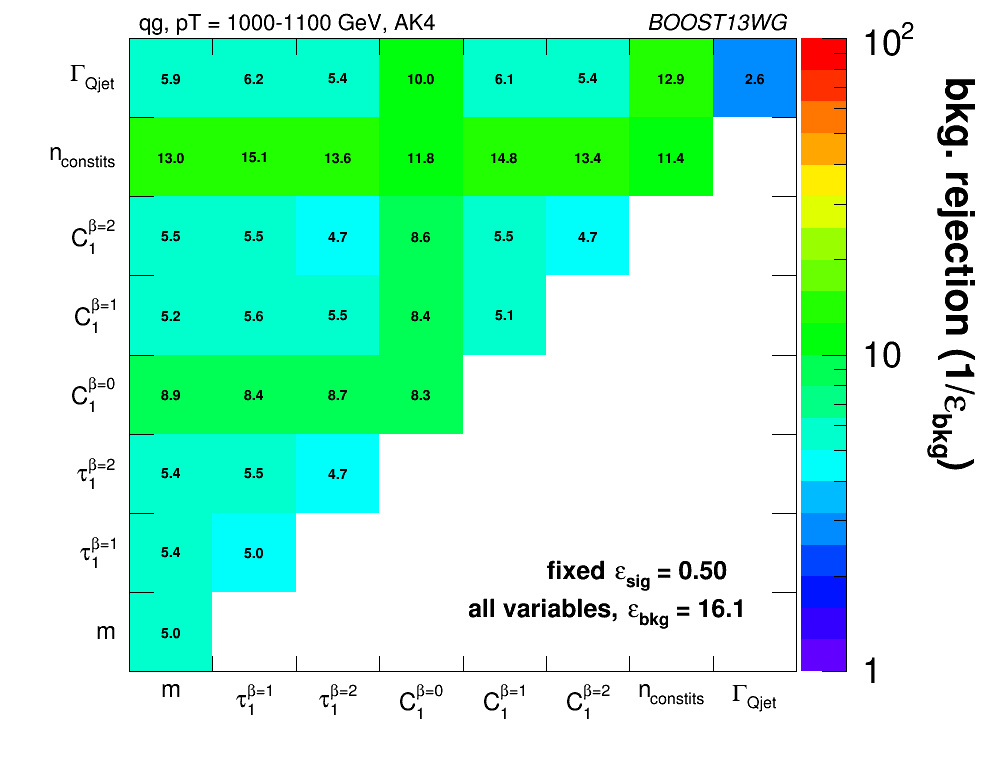
\includegraphics[width=0.48\textwidth]{./Figures/QGTagging/pT1000/AKtR04/effBkg2D.png}
%\includegraphics[width=0.4\textwidth]{./Figures/QGTagging/pT1000/AKtR04/Rocs_1D_single.png}\\
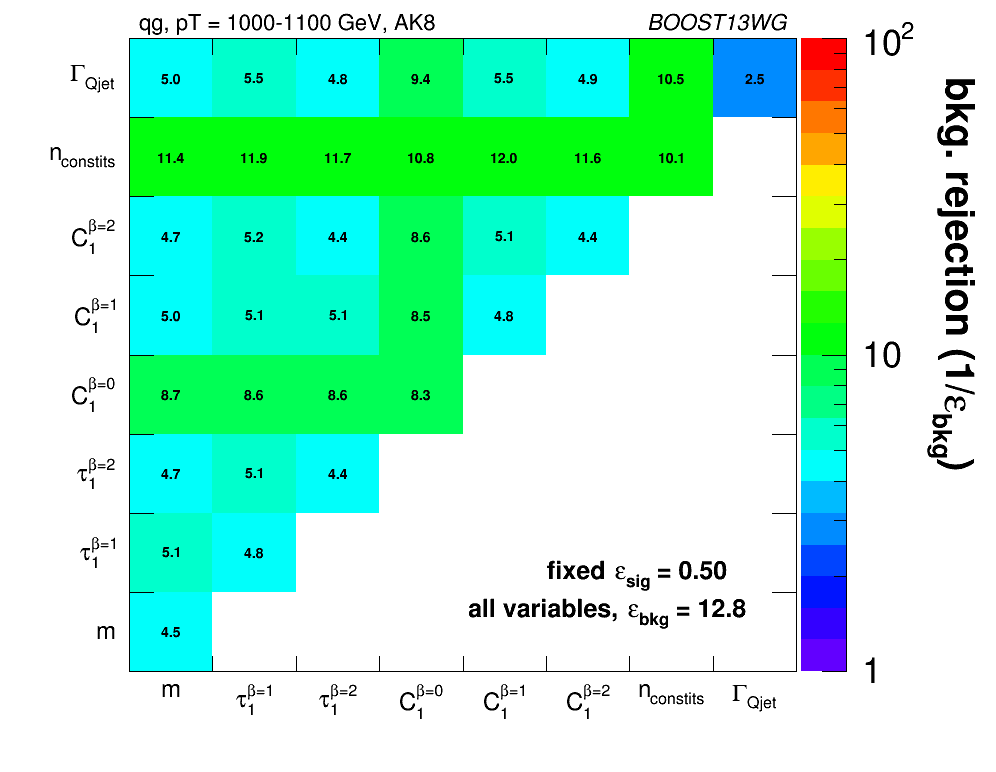
\includegraphics[width=0.48\textwidth]{./Figures/QGTagging/pT1000/AKtR08/effBkg2D.png}
%\includegraphics[width=0.4\textwidth]{./Figures/QGTagging/pT1000/AKtR08/Rocs_1D_single.png}\\
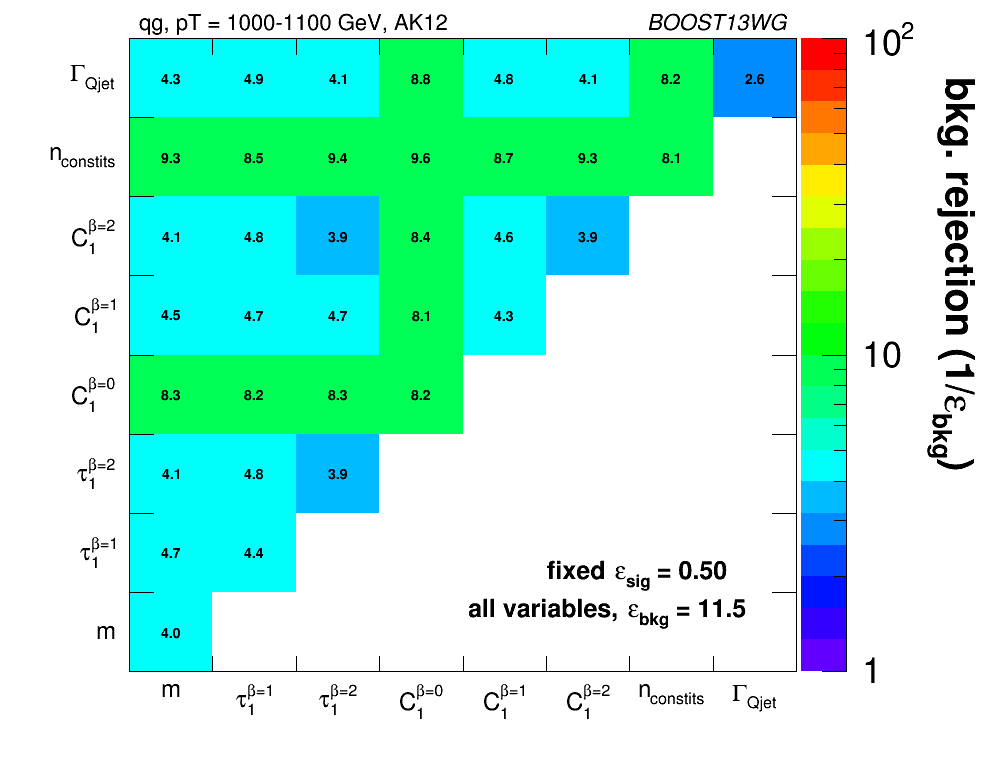
\includegraphics[width=0.48\textwidth]{./Figures/QGTagging/pT1000/AKtR12/effBkg2D.png}
%\includegraphics[width=0.4\textwidth]{./Figures/QGTagging/pT1000/AKtR12/Rocs_1D_single.png}\\
\caption{Gluon rejection defined as $1/\epsilon_{\rm gluon}$ when using each 2-variable combination 
as a tagger with 50\% acceptance for quark jets. Results are shown for
jets with $\pt=1-1.1 \TeV$ and
for (left) $R=0.4$; (centre) $R=0.8$; (right) $R=1.2$. The rejection obtained with a tagger that uses all variables is also shown
in the plots. }
\label{fig:qg_pt1000_comb}
\end{figure*}
As already observed in the previous section, $n_{\rm constits}$ is the most powerful single variable and
$\C{1}{\beta=0}$ follows closely. However, the gains are largely correlated; the combined performance of $n_{\rm constits}$ and $\C{1}{\beta=0}$ is generally poorer than combinations of $n_{\rm constits}$ with other jet substructure observables, such as $\tau_1$. Interestingly, in spite of the high correlation between $n_{\rm constits}$ and $\C{1}{\beta=0}$, the two-variable combinations of $n_{\rm constits}$ generally fare worse than two-variable combinations with $\C{1}{\beta=0}$ . In particular,
the combinations of $\tau^{\beta=1}_1$ or $\C{1}{\beta=1}$ with $n_{\rm constits}$ are capable of 
getting very  close to the rejection achievable through the use of all variables for $R=0.4$ and $R=0.8$.


 Tagger performance is generally better at small $R$. 
The overall loss in performance
with increasing $R$ can be seen in most single variables we study; this is expected, since more of the parton radiation is captured in the jet and more contamination from underlying event occurs, suppressing the differences between $q$/$g$ jets. 
The principal exceptions are $\C{1}{\beta=0}$ and 
the Q-jet mass volatility, which are both quite resilient to increasing $R$. For $\C{1}{\beta=0}$, this is due to the fact that the exponent on $\Delta R$ is zero, and so soft radiation at the periphery of the jet does not substantially change the distribution; as a result, the performance is largely independent of $R$.  Similarly, the soft radiation distant from the jet centre will be vetoed during pruning regardless of the cluster sequence, and so the $R$-dependence of $\Gamma_{\rm Qjet}$ is not significant.   ({\bf BS: Check my logic?}) Their combination, however, does perform slightly worse at larger $R$. ({\bf BS: I don't understand this, but it is a $\sim10\%$ effect, so maybe not too significant?}).
By contrast, $\tau_1^{(\beta=2)}$ and $\C{1}{\beta=2}$
are particularly sensitive to increasing R since, for $\beta=2$,
 large-angle emissions are given a larger weight. 

These observations are qualitatively similar across all ranges of $\pt$. Quantitatively, however,
there is a loss of rejection power for the taggers made of a combination of variables as the $\pt$ decreases. 
This can be observed in Fig.~\ref{fig:qg_akt4_comb} for anti-$\kT$ R=0.4 jets of different $\pt$s. 
\begin{figure*}
\centering
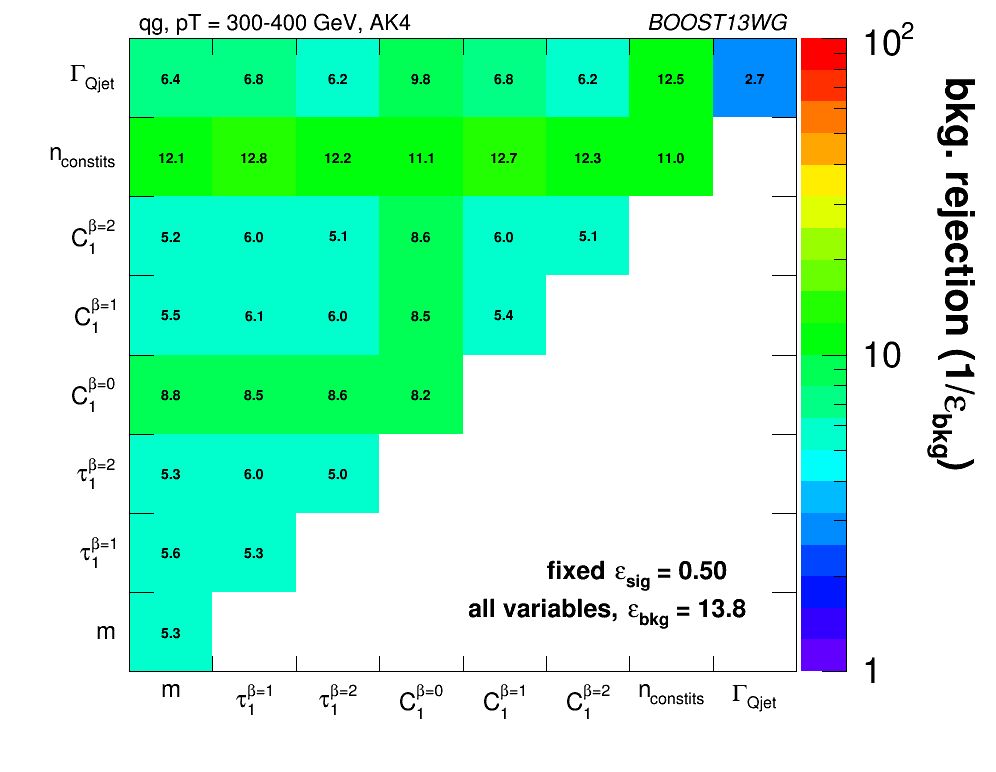
\includegraphics[width=0.48\textwidth]{./Figures/QGTagging/pT300/AKtR04/effBkg2D.png}
%\includegraphics[width=0.4\textwidth]{./Figures/QGTagging/pT1000/AKtR04/Rocs_1D_single.png}\\
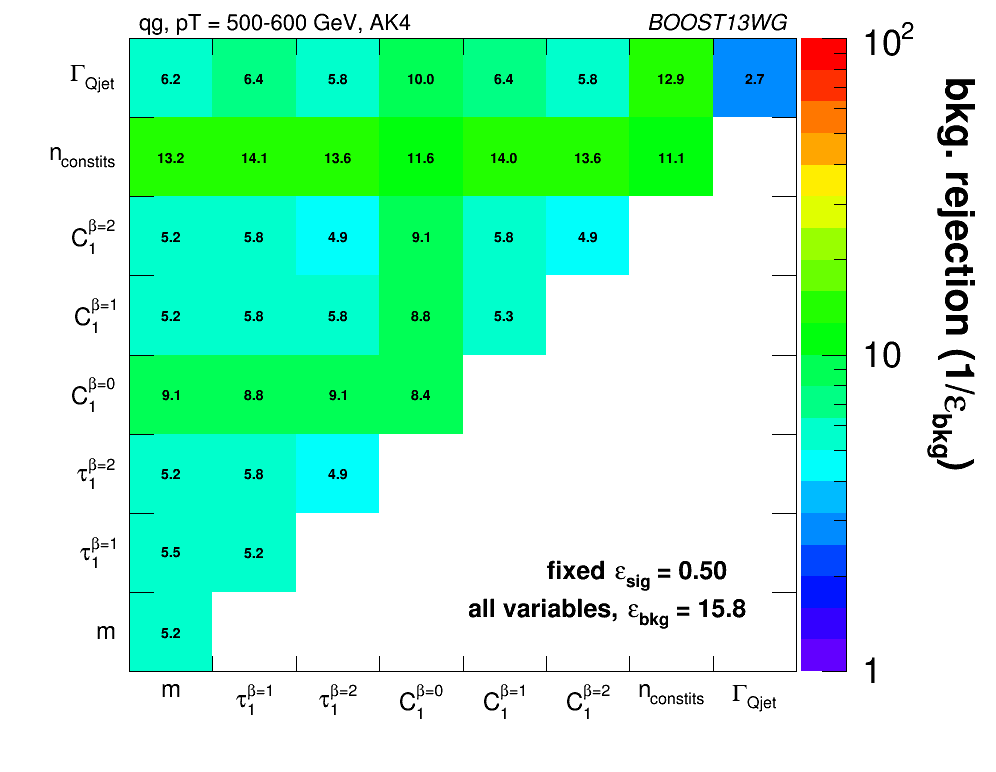
\includegraphics[width=0.48\textwidth]{./Figures/QGTagging/pT500/AKtR04/effBkg2D.png}
%\includegraphics[width=0.4\textwidth]{./Figures/QGTagging/pT1000/AKtR08/Rocs_1D_single.png}\\
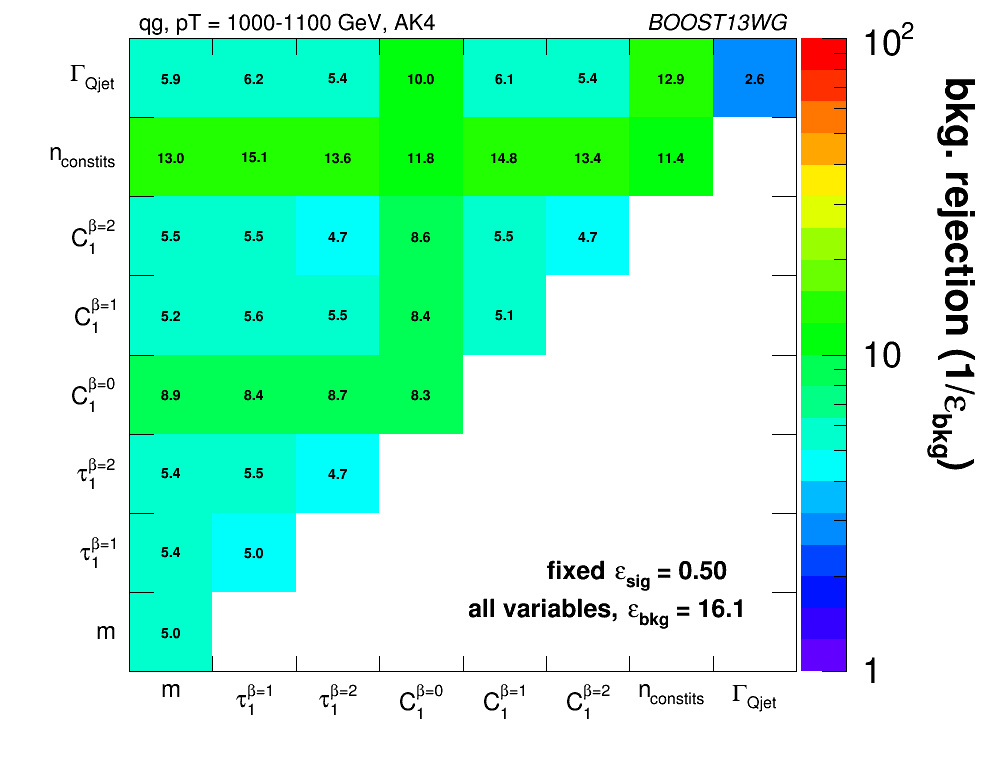
\includegraphics[width=0.48\textwidth]{./Figures/QGTagging/pT1000/AKtR04/effBkg2D.png}
%\includegraphics[width=0.4\textwidth]{./Figures/QGTagging/pT1000/AKtR12/Rocs_1D_single.png}\\
\caption{Gluon rejection defined as $1/\epsilon_{\rm gluon}$ when using each 2-variable combination 
as a tagger with 50\% acceptance for quark jets. Results are shown for R=0.4 jets with $\pt=300-400 \GeV$, 
$\pt=500-600 \GeV$ and $\pt=1-1.1 \TeV$. The rejection obtained with a tagger that uses all variables is also shown
in the plots. }
\label{fig:qg_akt4_comb}
\end{figure*}
Clearly, most single variables retain their gluon rejection potential at lower $\pt$. However, when combined
with other variables, the highest performing pairwise combinations lose ground with respect to other pairwise 
combinations. This is also reflected in the rejection of the tagger that uses a combination of all variables, which
is lower at lower $\pt$s. {\bf [do we understand this?]} ({\bf BS: This is a bit of a guess, but could it be that there is typically less radiation for low $\pt$, and so you're more sensitive to fluctuations; since you have less access to information, combinations of observables perform less well than at high $\pt$.})


%\subsection{QJets Volatility and $\ptd$ ($\C{1}{\beta=0}$)}

%Simple explanation of correlation, or why does combining volatility and $\ptd$ improve quark versus gluon discrimination.  $\ptd$ ($\C{1}{\beta=0}$) takes small (large) values for a jet with near-democratic energy sharing between particles and large (small) values when the energy of the jet is contained in a few particles.  Because we expect gluons to radiate more particles, we expect that $\ptd_g<\ptd_q$ (or ${\C{1}{\beta=0}}_g>{\C{1}{\beta=0}}_q$).  Now, we expect the volatility of gluon jets to be in general smaller than that of quark jets because there is a greater probability (by a factor of about $C_A/C_F=9/4$) that there was a relatively hard emission in a jet that is not groomed away.  By measuring both volatility and $\ptd$, we are sensitive to both regions of phase space: where a relatively hard emission dominates the mass of the jet as well as the region where many soft emissions set the jet mass.

\FloatBarrier

\section{Boosted $W$-Tagging}
\label{sec:wtagging}
In this section we study the performance of various jet algorithms in
combination with jet substructure variables/taggers in terms of the
identification of a boosted hadronically decaying $W$ signal. For each
jet algorithm we produce Receiver Operating Characteristic (ROC)
curves that elucidate the performance of various variables that are
capable of providing discrimination between a hadronic $W$ signal and
a QCD jet. These variables are then combined in a Boosted Decision Tree (BDT) and the performance of the resulting BDT discriminant
explored through ROC curves to understand the degree to which
variables are correlated and exploiting the same information. These
studies are repeated in different kinematic regimes, to explore both
the performance and correlations as a function of the jet boost, and
where substructure approaches may break down.

\subsection{Methodology}

These studies use the $X \rightarrow WW$ samples as signal and the XXX
samples to model the QCD background. 

Jets are reconstructed using the XXX jet algorithms described in the
previous section. The following event selection is then applied to these
samples....(presumably this will vary depending on which kinematic bin
is used, as will the actual samples used - maybe summarize in a table).

Figure~\ref{fig:pt500_basics_AKt_R08} shows
background versus signal in some basic kinematic
distributions. {\it Do we want to reweight signal kinematics to
background or vice versa? Do we want to study quarks/gluons separately?}

Go on to explain how we produce the ROC curves.

\begin{figure*}
\begin{center}
\subfigure[Leading jet
\pT]{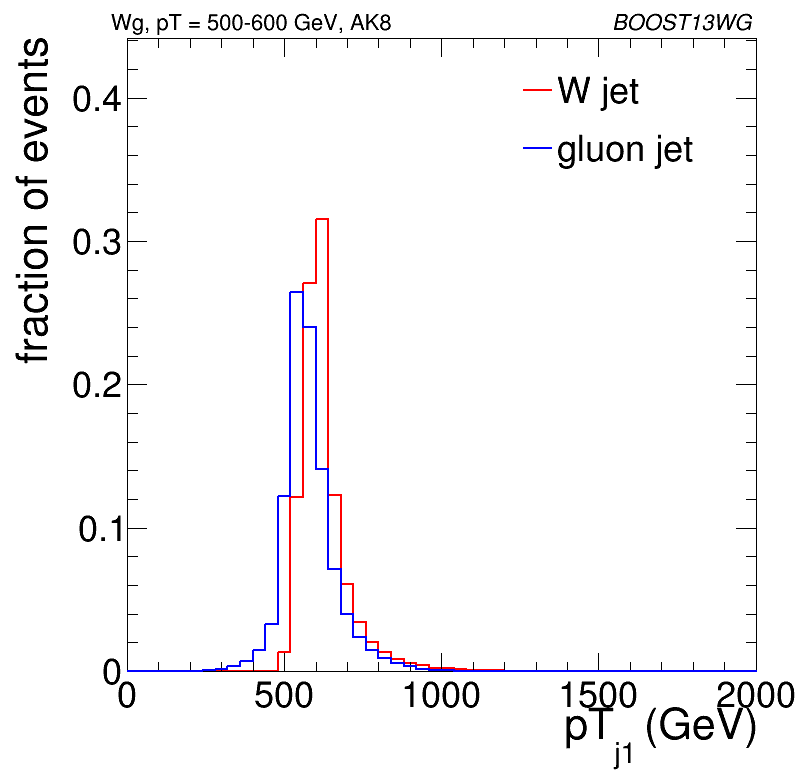
\includegraphics[width=0.48\textwidth]{./Figures/WTagging/pT500/AKtR08/jpt1.png}}
\subfigure[Sub-leading jet
\pT]{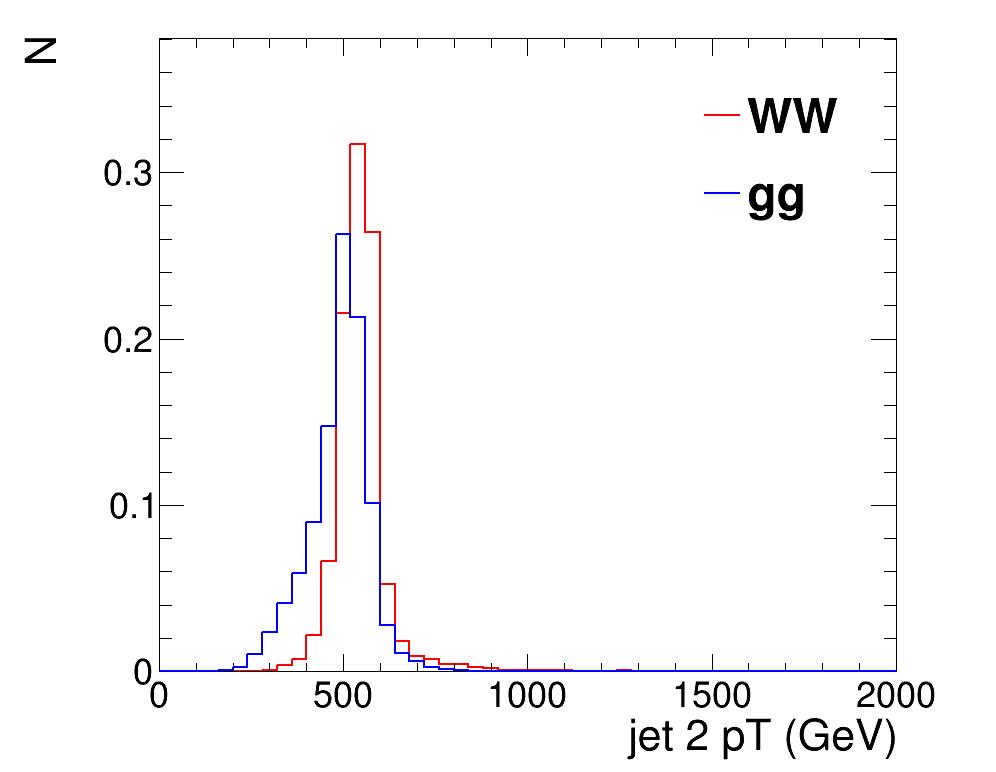
\includegraphics[width=0.48\textwidth]{./Figures/WTagging/pT500/AKtR08/jpt2.png}}
\subfigure[Leading jet
$\eta$]{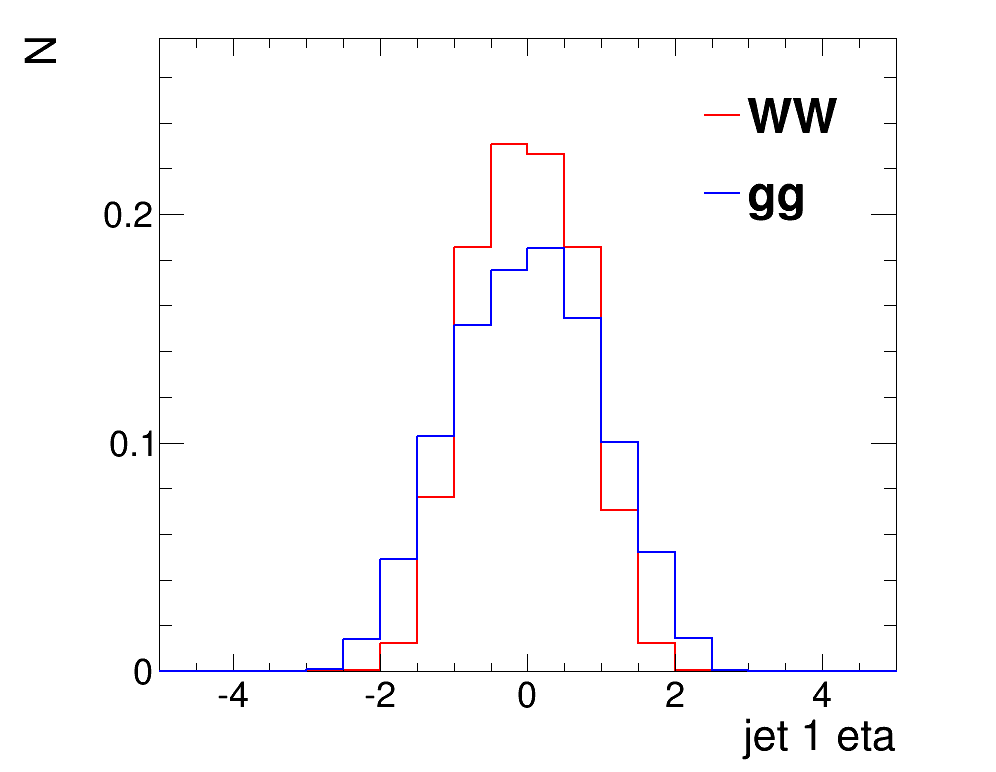
\includegraphics[width=0.48\textwidth]{./Figures/WTagging/pT500/AKtR08/jeta1.png}}
\subfigure[Sub-leading jet
$\eta$]{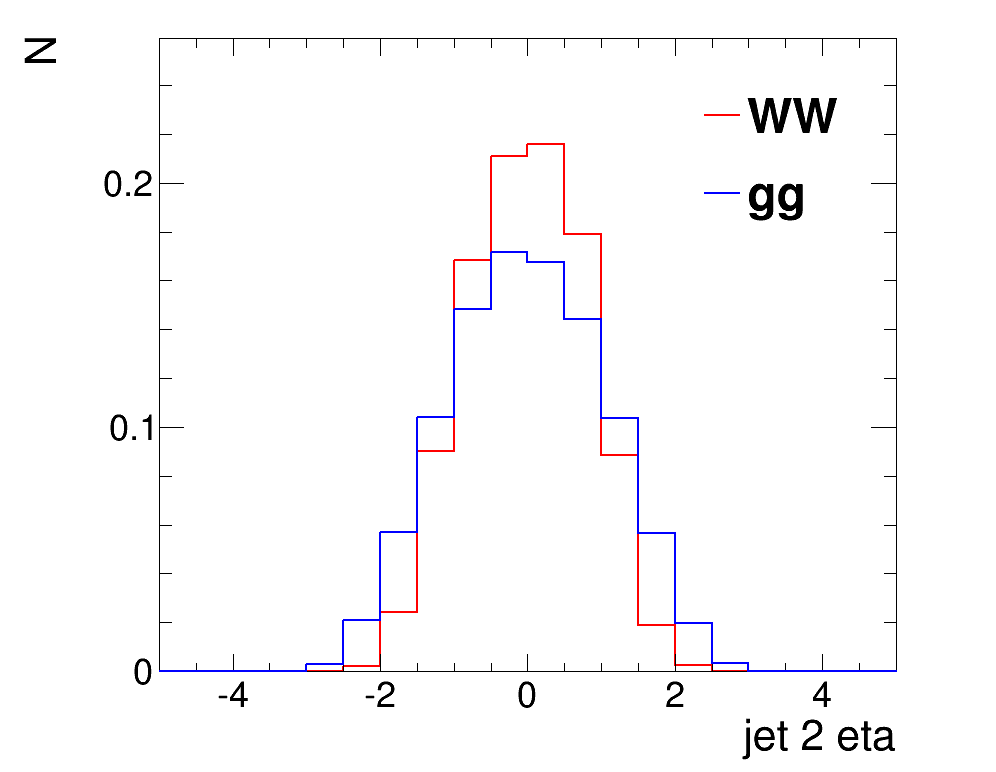
\includegraphics[width=0.48\textwidth]{./Figures/WTagging/pT500/AKtR08/jeta2.png}}
\caption{Comparisons of the QCD background to the WW signal in the \pt 500 GeV bin using the anti-\kT R=0.8 algorithm: basic
  kinematic distributons.}
\label{fig:pt500_basics_AKt_R08}
\end{center}
\end{figure*}


\subsection{Performance at Moderate Boosts}

(this section is to cover the $W$-tagging performance for jet \pT 200-300 GeV and
500-600 GeV using $\sqrt{s} = 8$ TeV samples)

\subsubsection{Single Variable Performance}

{\it Show plots of signal versus background for all single variables investigated}.

Figure~\ref{fig:pt500_mass_AKt_R08} the compares signal and background
 in the mass distributions for the different groomers, and Figure~\ref{fig:pt500_subst_AKt_R08}
in the different substructure variables. 

\begin{figure*}
\begin{center}
\subfigure[Ungroomed mass]{\includegraphics[width=0.48\textwidth]{./Figures/WTagging/pT500/AKtR08/jmass1.png}}
\subfigure[Pruned mass]{\includegraphics[width=0.48\textwidth]{./Figures/WTagging/pT500/AKtR08/h_mass_prun.png}}
\subfigure[Trimmed mass]{\includegraphics[width=0.48\textwidth]{./Figures/WTagging/pT500/AKtR08/h_mass_trim.png}}
\subfigure[mMDT mass]{\includegraphics[width=0.48\textwidth]{./Figures/WTagging/pT500/AKtR08/h_mass_mmdt.png}}
\subfigure[Soft-drop $\beta=2$ mass]{\includegraphics[width=0.48\textwidth]{./Figures/WTagging/pT500/AKtR08/h_mass_sdb2.png}}
\subfigure[Soft-drop $\beta=-1$ mass]{\includegraphics[width=0.48\textwidth]{./Figures/WTagging/pT500/AKtR08/h_mass_sdm1.png}}
\caption{Comparisons of the QCD background to the WW signal in the \pt 500 GeV bin using the anti-\kT R=0.8 algorithm: leading
  jet mass distributions.}
\label{fig:pt500_mass_AKt_R08}
\end{center}
\end{figure*}

\begin{figure*}
\begin{center}
\subfigure[$C_2^{\beta=1}$]{\includegraphics[width=0.48\textwidth]{./Figures/WTagging/pT500/AKtR08/h_c2_b1.png}}
\subfigure[$C_2^{\beta=2}$]{\includegraphics[width=0.48\textwidth]{./Figures/WTagging/pT500/AKtR08/h_c2_b2.png}}
\subfigure[$\Gamma_{Qjet}$]{\includegraphics[width=0.48\textwidth]{./Figures/WTagging/pT500/AKtR08/h_qjetVol.png}}
\subfigure[$\tau_{21}^{\beta=1}$]{\includegraphics[width=0.48\textwidth]{./Figures/WTagging/pT500/AKtR08/h_tau21_b1.png}}
\subfigure[$\tau_{21}^{\beta=2}$]{\includegraphics[width=0.48\textwidth]{./Figures/WTagging/pT500/AKtR08/h_tau21_b2.png}}
\caption{Comparisons of the QCD background to the WW signal in the \pt 500 GeV bin using the anti-\kT R=0.8 algorithm:
  substructure variables.}
\label{fig:pt500_subst_AKt_R08}
\end{center}
\end{figure*}


Figure~\ref{fig:pt500_single_AKt_R08} shows the single variable ROC curves in
the \pT 500 GeV bin for the anti-\kT R=0.8 algorithm, compared to the
ROC curve for a BDT combination of all the variables. One can see that
the best performant single variables for a reasonable signal
efficiency are the groomed/filtered masses, which all have a similar
level of performance with the exception of the soft drop mass with $\beta=-1$. {\it Would be good to split this into two plots, one
using the masses and one for other variables, or somehow make the mass
and other variable curves more distinct from one another by using same
colour for all the mass curves}.

{\it We want to look also at:
\begin{itemize}
\item Dependence on R. So have the same single variable ROC for
e.g. R=1.2, R=0.4. Then possibly have another plot which compares the
best single variable (e.g. groomed mass) for
different R.
\item Dependence on pT. Again want to repeat the plot for different
kinematic bins, and then have a plot which compares the best
performance in each kinematic bin to see the dependence of performance
on kinematics.
\end{itemize}
}

\begin{figure*}
\begin{center}
\includegraphics[width=0.8\textwidth]{./Figures/WTagging/pT500/AKtR08/Rocs_1D_single.png}
\caption{The ROC curve for all single variables considered for $W$
tagging in the \pt 500 GeV bin using the anti-\kT R=0.8 algorithm.}
\label{fig:pt500_single_AKt_R08}
\end{center}
\end{figure*}

Figure~\ref{fig:pt500_single_AKt_R12} shows the single variable ROC curves in
the \pT 500 GeV bin for the anti-\kT R=1.2 algorithm, compared to the
ROC curve for a BDT combination of all the variables. Comparing to
Figure~\ref{fig:pt500_single_AKt_R08}, one can see that the
performance of the groomed masses is quite similar. However, the
performance of the other non-mass substructure variables is markedly
different, and better in the R=0.8 case.

\begin{figure*}
\begin{center}
\includegraphics[width=0.8\textwidth]{./Figures/WTagging/pT500/AKtR12/Rocs_1D_single.png}
\caption{The ROC curve for all single variables considered for $W$
tagging in the \pt 500 GeV bin using the anti-\kT R=1.2 algorithm.}
\label{fig:pt500_single_AKt_R12}
\end{center}
\end{figure*}


\subsubsection{Combined Performance}

\subsubsection*{Mass + X Performance}

Figure~\ref{fig:pt500_masscomb_AKt_R08} shows the BDT combinations of each mass variable with every other
variable considered in the \pt 500 GeV bin using the anti-\kT R=0.8
algorithm. {\it Can we drop the combinations of mass + mass
from these plots to make them clearer? Also would be good to put the
single variable mass curve on these plots, so you can see how much
improvement the combination gives, and the ``all variables'' curve.}

No combination with other variables can recover the poor performance
of the ungroomed mass and the soft drop mass with $\beta=-1$. The
other groomed/filtered masses are all most improved by combination
with the $C_{2}^{\beta=1}$ energy correlation
function. Figure~\ref{fig:pt500_2d_mmdt_AKt_R08} shows the 2-D
correlation plots between the mMDT mass and the $C_{2}^{\beta=1}$,
$\Gamma_{Qjet}$ and $\tau_{21}^{\beta=1}$ variables. One can clearly
see that there is substantially less correlation between the mass and
$C_{2}^{\beta=1}$ than the other variables. Similar results are seen
for the other groomed masses.

\begin{figure*}
\begin{center}
\subfigure[Ungroomed mass + X]{\includegraphics[width=0.48\textwidth]{./Figures/WTagging/pT500/AKtR08/Rocs_1D_jmass.png}}
\subfigure[Trimmed mass + X]{\includegraphics[width=0.48\textwidth]{./Figures/WTagging/pT500/AKtR08/Rocs_1D_j_mass_trim.png}}
\subfigure[Pruned mass + X]{\includegraphics[width=0.48\textwidth]{./Figures/WTagging/pT500/AKtR08/Rocs_1D_j_mass_prun.png}}
\subfigure[Soft drop mass ($\beta=-1$) +X]{\includegraphics[width=0.48\textwidth]{./Figures/WTagging/pT500/AKtR08/Rocs_1D_j_mass_sdm1.png}}
\subfigure[Soft drop mass ($\beta=2$) + X]{\includegraphics[width=0.48\textwidth]{./Figures/WTagging/pT500/AKtR08/Rocs_1D_j_mass_sdb2.png}}
\subfigure[mMDT mass + X]{\includegraphics[width=0.48\textwidth]{./Figures/WTagging/pT500/AKtR08/Rocs_1D_j_mass_mmdt.png}}
\caption{The BDT combinations of each mass variable with every other
variable considered in the \pt 500 GeV bin using the anti-\kT R=0.8 algorithm.}
\label{fig:pt500_masscomb_AKt_R08}
\end{center}
\end{figure*}

\begin{figure*}
\begin{center}
\subfigure[mMDT mass vs $C_2^{\beta=1}$]{\includegraphics[width=0.48\textwidth]{./Figures/WTagging/pT500/AKtR08/h2d_jc2_b1_j_mass_mmdt_gg.png}}
\subfigure[mMDT mass vs $\Gamma_{Qjet}$]{\includegraphics[width=0.48\textwidth]{./Figures/WTagging/pT500/AKtR08/h2d_j_qjetVol_j_mass_mmdt_gg.png}}
\subfigure[mMDT mass vs $\tau_{21}^{\beta=1}$]{\includegraphics[width=0.48\textwidth]{./Figures/WTagging/pT500/AKtR08/h2d_jtau21_b1_j_mass_mmdt_gg.png}}
\caption{2-D plots showing the correlation between mMDT mass and
  various substructure variables in the \pt 500 GeV bin using the
  anti-\kT R=0.8 algorithm in the gg sample.}
\label{fig:pt500_2d_mmdt_AKt_R08}
\end{center}
\end{figure*}

Figure~\ref{fig:pt500_masscomb_AKt_R12} shows the BDT combinations of
the bset performant groomed masses with every other
variable considered in the \pt 500 GeV bin using the anti-\kT R=1.2
algorithm. Interestingly, the groomed masses are now all most improved by combination
with the $\tau_{21}^{\beta=1}$ variable, in contrast with
$C_{2}^{\beta=1}$ which performed best for the smaller radius of
R=0.8. One can see from Figure~\ref{fig:pt500_single_AKt_R12} that the
single variable discrimination of $\tau_{21}^{\beta=1}$ and
$C_{2}^{\beta=1}$ changes quite markedly when the distance parameter R
is varied, although in both cases $C_{2}^{\beta=1}$ is a better single
variable discriminant (except for very high signal
efficiencies). Figure~\ref{fig:pt500_2d_mmdt_AKt_R12} shows the 2-D
correlation plots between between the mMDT mass and the $C_{2}^{\beta=1}$,
$\Gamma_{Qjet}$ and $\tau_{21}^{\beta=1}$ variables for the R=1.2
case. It is hard to see a substantial difference in the correlations
here versus Figure~\ref{fig:pt500_2d_mmdt_AKt_R08}, but perhaps
$C_{2}^{\beta=1}$ is marginally more correlated with the mass for
R=1.2 compared to R=0.8.

{\it Now show a plot which compares on one plot the best combined performance for
each groomed mass + X for both R=0.8 and 1.2 cases e.g. mass +
$C_{2}^{\beta=1}$ for R=0.8 and mass + $\tau_{21}^{\beta=1}$ for R=1.2,
  and draw on also the
all variables curve for both R=0.8,1.2. 
Then we can see if there is much dependence on choice of mass once you
combine with another variable, and compare directly the two distance parameters.
This plot is just for
one kinematic bin, we should make the same plot for others.}

{\it Repeat these studies for different R and different kinematic
bins. Finally make plots which compare best combined performance for
different R and kinematics.}

{\it Do we want to look at other combinations of variables which don't
involve mass? Practically I think we will always be making mass + X though.}



\begin{figure*}
\begin{center}
%\subfigure[Ungroomed mass + X]{\includegraphics[width=0.48\textwidth]{./Figures/WTagging/pT500/AKtR12/Rocs_1D_jmass.png}}
\subfigure[Trimmed mass + X]{\includegraphics[width=0.48\textwidth]{./Figures/WTagging/pT500/AKtR12/Rocs_1D_j_mass_trim.png}}
\subfigure[Pruned mass + X]{\includegraphics[width=0.48\textwidth]{./Figures/WTagging/pT500/AKtR12/Rocs_1D_j_mass_prun.png}}
%\subfigure[Soft drop mass ($\beta=-1$) +X]{\includegraphics[width=0.48\textwidth]{./Figures/WTagging/pT500/AKtR12/Rocs_1D_j_mass_sdm1.png}}
\subfigure[Soft drop mass ($\beta=2$) + X]{\includegraphics[width=0.48\textwidth]{./Figures/WTagging/pT500/AKtR12/Rocs_1D_j_mass_sdb2.png}}
\subfigure[mMDT mass + X]{\includegraphics[width=0.48\textwidth]{./Figures/WTagging/pT500/AKtR12/Rocs_1D_j_mass_mmdt.png}}
\caption{The BDT combinations of each mass variable with every other
variable considered in the \pt 500 GeV bin using the anti-\kT R=1.2 algorithm.}
\label{fig:pt500_masscomb_AKt_R12}
\end{center}
\end{figure*}

\begin{figure*}
\begin{center}
\subfigure[mMDT mass vs $C_2^{\beta=1}$]{\includegraphics[width=0.48\textwidth]{./Figures/WTagging/pT500/AKtR12/h2d_jc2_b1_j_mass_mmdt_gg.png}}
\subfigure[mMDT mass vs $\Gamma_{Qjet}$]{\includegraphics[width=0.48\textwidth]{./Figures/WTagging/pT500/AKtR12/h2d_j_qjetVol_j_mass_mmdt_gg.png}}
\subfigure[mMDT mass vs $\tau_{21}^{\beta=1}$]{\includegraphics[width=0.48\textwidth]{./Figures/WTagging/pT500/AKtR12/h2d_jtau21_b1_j_mass_mmdt_gg.png}}
\caption{2-D plots showing the correlation between mMDT mass and
  various substructure variables in the \pt 500 GeV bin using the
  anti-\kT R=1.2 algorithm in the gg sample.}
\label{fig:pt500_2d_mmdt_AKt_R12}
\end{center}
\end{figure*}


\subsubsection*{Mass + Mass Performance}

It's interesting also to study and understand how the different
groomed masses relate to each other and how they are correlated.

Figures~\ref{fig:pt500_2d_massQQ_AKt_R08} and Figures~\ref{fig:pt500_2d_massGG_AKt_R08} shows 2-D correlation plots of
the different types of groomed mass in the \pt 500 GeV bin using the anti-\kT R=0.8
algorithm.

{\it Worth also showing some ROC curves for mass + mass combinations?}


\begin{table*}[htbp!]
\centering
%\setlength\fboxsep{0pt}
%\setlength\fboxrule{0.25pt}
\caption{Action of various groomers on the jet mass distribution in the different phase space regions.  For pruning, $a_\text{prune} = \zcut R_0$ and for trimming $a_\text{trim} = \sqrt{\zcut} R_\text{sub}$.}
\begin{tabular}{c|c|c|c|c} 
Action & Pruning & Trimming & mMDT & SD ($\beta > 0$) \\ \hline
$m>\sqrt{\zcut}R_0 p_T$  &  $-$ & $-$ &  $-$  & $-$ \\ \hline
\parbox[c][3em][c]{7em}{$m<\sqrt{\zcut}R_0 p_T$\\$m>a_x p_T$} & \parbox[c][3em][c]{6em}{cuts soft \& \\ soft-collinear}  & \parbox[c][3em][c]{6em}{cuts soft \& \\ soft-collinear} & \parbox[c][3em][c]{6em}{cuts soft \& \\ soft-collinear} & \parbox[c][5em][c]{7em}{cuts soft \& \\ partially ($\beta$) \\ on soft-collinear}  \\ \hline
$m<a_x p_T$ & \parbox[c][5em][c]{7em}{cuts partially \\ on both soft \& \\  soft-collinear}   &$-$ & \parbox[c][3em][c]{6em}{cuts soft \& \\ soft-collinear} & \parbox[c][5em][c]{7em}{cuts soft \& \\ partially ($\beta$) \\ on soft-collinear} 
\end{tabular}
\label{tab:boostedtoprates}
\end{table*}


\begin{figure*}
\begin{center}
\subfigure[Trimmed mass vs Soft drop mass ($\beta=2$)]{\includegraphics[width=0.48\textwidth]{./Figures/WTagging/pT500/AKtR08/WvsQ/h2d_j_mass_trim_j_mass_sdb2_WW_onSame.png}}
\subfigure[Trimmed mass vs Pruned mass]{\includegraphics[width=0.48\textwidth]{./Figures/WTagging/pT500/AKtR08/WvsQ/h2d_j_mass_trim_j_mass_prun_WW_onSame.png}}
\subfigure[Trimmed mass vs mMDT mass]{\includegraphics[width=0.48\textwidth]{./Figures/WTagging/pT500/AKtR08/WvsQ/h2d_j_mass_trim_j_mass_mmdt_WW_onSame.png}}
\subfigure[mMDT mass vs Soft drop mass ($\beta=2$)]{\includegraphics[width=0.48\textwidth]{./Figures/WTagging/pT500/AKtR08/WvsQ/h2d_j_mass_mmdt_j_mass_sdb2_WW_onSame.png}}
\subfigure[Pruned mass vs Soft drop mass ($\beta=2$)]{\includegraphics[width=0.48\textwidth]{./Figures/WTagging/pT500/AKtR08/WvsQ/h2d_j_mass_prun_j_mass_sdb2_WW_onSame.png}}
\subfigure[mMDT mass vs Pruned mass]{\includegraphics[width=0.48\textwidth]{./Figures/WTagging/pT500/AKtR08/WvsQ/h2d_j_mass_mmdt_j_mass_prun_WW_onSame.png}}
\caption{2-D plots showing the correlation between different types of
  groomed mass in the \pt 500 GeV bin using the anti-\kT R=0.8
  algorithm, separately for the jets in the $X \rightarrow WW$ sample and the
  jets in the quark-quark sample.}
\label{fig:pt500_2d_massQQ_AKt_R08}
\end{center}
\end{figure*}

\begin{figure*}
\begin{center}
\subfigure[Trimmed mass vs Soft drop mass ($\beta=2$)]{\includegraphics[width=0.48\textwidth]{./Figures/WTagging/pT500/AKtR08/WvsG/h2d_j_mass_trim_j_mass_sdb2_WW_onSame.png}}
\subfigure[Trimmed mass vs Pruned mass]{\includegraphics[width=0.48\textwidth]{./Figures/WTagging/pT500/AKtR08/WvsG/h2d_j_mass_trim_j_mass_prun_WW_onSame.png}}
\subfigure[Trimmed mass vs mMDT mass]{\includegraphics[width=0.48\textwidth]{./Figures/WTagging/pT500/AKtR08/WvsG/h2d_j_mass_trim_j_mass_mmdt_WW_onSame.png}}
\subfigure[mMDT mass vs Soft drop mass ($\beta=2$)]{\includegraphics[width=0.48\textwidth]{./Figures/WTagging/pT500/AKtR08/WvsG/h2d_j_mass_mmdt_j_mass_sdb2_WW_onSame.png}}
\subfigure[Pruned mass vs Soft drop mass ($\beta=2$)]{\includegraphics[width=0.48\textwidth]{./Figures/WTagging/pT500/AKtR08/WvsG/h2d_j_mass_prun_j_mass_sdb2_WW_onSame.png}}
\subfigure[mMDT mass vs Pruned mass]{\includegraphics[width=0.48\textwidth]{./Figures/WTagging/pT500/AKtR08/WvsG/h2d_j_mass_mmdt_j_mass_prun_WW_onSame.png}}
\caption{2-D plots showing the correlation between different types of
  groomed mass in the \pt 500 GeV bin using the anti-\kT R=0.8
  algorithm, separately for the jets in the $X \rightarrow WW$ sample and the
  jets in the gluon-gluon sample.}
\label{fig:pt500_2d_massGG_AKt_R08}
\end{center}
\end{figure*}


\subsection{Performance at High Boosts}

(this section is to cover the $W$-tagging performance for jet \pT 1-1.1 TeV and
$>$ 1.5 TeV using $\sqrt{s} = 14$ TeV samples)

{\it Maybe we don't need to divide into different medium/high boost sections.}





\FloatBarrier

\section{Top Tagging}
\label{sec:toptagging}
In this section, we investigate the identification of boosted top quarks using jet substructure. Boosted top quarks result in large-radius jets with complex substructure, containing a $b$-subjet and a boosted $W$. The additional kinematic handles coming from the reconstruction of the $W$ mass and $b$-tagging allow a very high degree of discrimination of top quark jets from QCD backgrounds. As a consequence of the many kinematic differences between top and QCD jets, top taggers are typically complex, with a couple of input parameters necessary for any given algorithm. We study the variation in performance of top tagging techniques with respect to jet \pt and $R$, re-optimizing the tagger inputs for each kinematic range and jet radius considered. We also investigate the effects of combining dedicated top tagging algorithms with other jet substructure variables, giving insight into the correlations among top-tagging variables. 

\subsection{Methodology}\label{sec:topmethod}

We use the top quark MC samples for each bin described in Section \ref{sec:top-samples}. The analysis  relies on \textsc{FastJet} 3.0.3 for jet clustering and
calculation of jet substructure variables. Jets are clustered using the \antikt algorithm, and only the leading jet is used in each analysis. To ensure similar $\pt$ spectra in each bin an upper and lower $\pt$ cut are applied to each sample after jet clustering. The bins in leading jet $\pt$
 for top tagging are 600-700 \GeV, 1-1.1 \TeV, and
1.5-1.6 TeV. Jets are clustered with radii $R=0.4$, 0.8, and 1.2; $R=0.4$ jets are only studied in the 1.5-1.6 TeV bin
because the top decay products are all contained within an $R=0.4$ jet for top quarks with this boost.

We study a number of top-tagging strategies, which can be divided into two distinct categories. In the first category are dedicated top-tagging algorithms, which aim to directly reconstruct the top and $W$ candidates in the top decay. In particular, we study:
%
\begin{enumerate}
\item HEPTopTagger
\item Johns Hopkins Tagger (JH)
\item Trimming with $W$-identification
\item Pruning with $W$-identification
\end{enumerate}
%
as described in Section~\ref{sec:taggers}. The top mass, \topmass, is the mass of the groomed jet. All of the above taggers and groomers incorporate a step to remove contributions from the underlying event and other soft radiation.

In the second category are individual jet substructure variables that are sensitive to the radiation pattern within the jet, which we refer to as ``jet-shape variables''. While the most sensitive top-tagging variables are typically sensitive to three-pronged radiation, we also consider variables sensitive to two-pronged radiation in the limit where the $W$ is very boosted and its subjets overlap. The variables we consider are:
%
\begin{itemize}
\item The ungroomed jet mass.
\item $N$-subjettiness ratios \tautwoone and \tauthreetwo, using the ``winner-takes-all'' axes definition.
\item 2-point energy correlation function ratios $C_2^{\beta=1}$ and $C_3^{\beta=1}$.
\item The pruned Qjet mass volatility, $\Gamma_{\rm Qjet}$.
\end{itemize}
%
Several of these variables were also considered earlier for $q/g$-tagging and $W$-tagging.

To study the correlation among the above top-tagging variables, we consider combinations of the mass-recon-struction methods with the shape variables.
For multivariate analyses, we combine the relevant tagger output variables and/or jet shapes into a BDT, as described in Section~\ref{sec:multivariate}. In the case of the HepTopTagger and JH tagger, the algorithms produce three output variables ($\topmass$, $\wmass$ and helicity angle) that can be used to discriminate top jets from QCD. Both taggers also explicitly rejects jets that do not meet basic selection criteria. The trimming and pruning algorithms as used here produce two outputs, $\topmass$ and $\wmass$, and the grooming algorithms may not return a top candidate if a suitable $W$ candidate cannot be found (as described in Section~\ref{sec:multivariate}). Additionally, because each tagger has two input parameters, we scan over reasonable values of the input parameters to determine the optimal value that gives the largest background rejection for each top tagging signal efficiency. This allows a direct comparison of the optimized version of each tagger. The input parameter values scanned for the various algorithms are:
%
\begin{itemize}
\item {\bf HEPTopTagger:} $m\in[30,100]$ \GeV, $\mu\in[0.5,1]$
\item {\bf JH Tagger:} $\delta_p\in[0.02,0.15]$, $\delta_R\in[0.07,0.2]$
\item {\bf Trimming:} $f_{\rm cut}\in[0.02,0.14]$, $R_{\rm trim}\in[0.1,0.5]$
\item {\bf Pruning:} $z_{\rm cut}\in[0.02,0.14]$, $R_{\rm cut}\in[0.1,0.6]$
\end{itemize}
%
We also investigate the degradation in performance of the top-tagging variables when moving away from the optimal parameter choice.

\subsection{Single-Observable Performance}\label{sec:single_variable}
We begin by investigating the behaviour of individual jet substructure variables. Because of the rich, three-pronged structure of the top decay, it is expected that combinations of masses and jet shapes will far outperform single variables in identifying boosted tops. However, a study of the top-tagging performance of single variables facilitates a direct comparison with the $W$ tagging results in Section \ref{sec:wtagging}, and also allows a straightforward examination of the performance of each observable for different $\pt$ and jet radius.

Top-tagging observable performance is quantified using ROC curves. Figure~\ref{fig:single_variable_ROC} shows the ROC curves for each of the top-tagging variables, with the bare (ungroomed) jet mass also plotted for comparison. The jet-shape variables all perform substantially worse than jet mass; this is in contrast with $W$ tagging, for which several variables are competitive with or perform better than jet mass (see, for example, Figures~\ref{fig:pt500_comb2D_08}, \ref{fig:pt1000_comb2D_04} and~\ref{fig:pt1000_comb2D_08}).
To understand why this is the case, consider $N$-subjettiness:~the $W$ is two-pronged and the top is three-pronged, and so we expect $\tau_{21}$ and $\tau_{32}$ to be the best-performant $N$-subjettiness ratio, respectively. However, a cut to select small values of $\tau_{21}$  necessarily also selects for 
jets with large $\tau_1$, which is strongly correlated with jet mass, up to Sudakov-suppressed contributions. Therefore, $\tau_{21}$ combines both mass and shape information to some extent. By contrast, and as is clear in Figure~\ref{fig:single_variable_ROC_shape}, the best shape for top tagging is $\tau_{32}$, which contains no information on the jet mass. It is therefore unsurprising that the  shapes most useful for top tagging are less sensitive to the jet mass, and under-perform relative to the corresponding variables for $W$ tagging.

\begin{figure*}
\centering
\subfigure[Jet shapes]{\includegraphics[width=0.49\textwidth]{./Figures/TTagging/single_variable/pT.1TeV.R.0.8/Rocs_shape.pdf}\label{fig:single_variable_ROC_shape}}
\subfigure[top mass]{\includegraphics[width=0.49\textwidth]{./Figures/TTagging/single_variable/pT.1TeV.R.0.8/Rocs_top_mass.pdf}\label{fig:single_variable_ROC_topmass}}
\subfigure[$W$ mass]{\includegraphics[width=0.49\textwidth]{./Figures/TTagging/single_variable/pT.1TeV.R.0.8/Rocs_w_mass.pdf}\label{fig:single_variable_ROC_wmass}}
\caption{Comparison of single-variable top-tagging performance in the $\pt= 1-1.1$ GeV bin using the anti-\kT, R=0.8 algorithm.}
\label{fig:single_variable_ROC}
\end{figure*}

Of the two top-tagging algorithms, it is apparent from Figure~\ref{fig:single_variable_ROC} that the Johns Hopkins tagger out-performs the HEPTopTagger in terms of its background rejection at fixed signal efficiency for both the top and $W$ candidate masses; this is expected, as the HEPTopTagger was designed to reconstruct moderate-\pt top jets in $ttH$ events (for a proposed high-\pt variant of the HEPTopTagger, see \cite{Schaetzel:2013vka}). In Figure~\ref{fig:topmass_histogram_HEP_JH}, we show the histograms for the top mass output from the JH and HEPTopTagger for different $R$ in the \pt =  1.5-1.6 TeV bin, and in Figure~\ref{fig:topmass_histogram_HEP_JH_pT} for different \pt at $R=0.8$, optimized at a signal efficiency of 30\%. 
A particular feature of the HepTopTagger algorithm is that, after the jet is filtered to select the five hardest subjets, the three subjets are chosen which most closely reconstruct the top mass. This requirement tends to shape a peak in the QCD background around $m_t$ for the HEPTopTagger, as can be seen from Figures~\ref{fig:topmass_histogram_HEP_R12} and~\ref{fig:topmass_histogram_HEP_pT15}; this is the likely reason for the better performance of the JH tagger, which has no such requirement.
%One can see from these figures that the likely reason for the better performance of the JH tagger is that, in the HEPTopTagger algorithm, the jet is filtered to select the five hardest subjets, and then three subjets are chosen which most closely reconstruct the top mass. This requirement tends to shape a peak in the QCD background around $m_t$ for the HEPTopTagger, while the JH tagger has no such requirement. 
It has been suggested  \cite{Anders:2013oga} that performance in the HEPTopTagger may be improved by selecting the three subjets reconstructing the top only among those that pass the $W$ mass constraints, which somewhat reduces the shaping of the background. The discrepancy between the JH and HEPTopTaggers is more pronounced  at higher $\pt$ and larger jet radius (see Figures~\ref{fig:ptcomparison_singletopmass_top} and \ref{fig:Rcomparison_singletopmass_top}). 

\begin{figure*}
\centering
\subfigure[JH, $R=0.4$]{\includegraphics[width=0.245\textwidth]{./Figures/TTagging/single_variable/pT.1.5TeV.R.0.4/h_JH_mt_opt_mt.pdf}}
\subfigure[HEP, $R=0.4$]{\includegraphics[width=0.245\textwidth]{./Figures/TTagging/single_variable/pT.1.5TeV.R.0.4/h_HEP_mt_opt_mt.pdf}}
\subfigure[JH, $R=1.2$]{\includegraphics[width=0.245\textwidth]{./Figures/TTagging/single_variable/pT.1.5TeV.R.1.2/h_JH_mt_opt_mt.pdf}}
\subfigure[HEP, $R=1.2$]{\includegraphics[width=0.245\textwidth]{./Figures/TTagging/single_variable/pT.1.5TeV.R.1.2/h_HEP_mt_opt_mt.pdf}\label{fig:topmass_histogram_HEP_R12}}\\
\subfigure[prune, $R=0.4$]{\includegraphics[width=0.245\textwidth]{./Figures/TTagging/single_variable/pT.1.5TeV.R.0.4/h_prun_R_0_4.pdf}}
\subfigure[trim, $R=0.4$]{\includegraphics[width=0.245\textwidth]{./Figures/TTagging/single_variable/pT.1.5TeV.R.0.4/h_trim_R_0_4.pdf}}
\subfigure[prune, $R=1.2$]{\includegraphics[width=0.245\textwidth]{./Figures/TTagging/single_variable/pT.1.5TeV.R.1.2/h_prun_R_1_2.pdf}}
\subfigure[trim, $R=1.2$]{\includegraphics[width=0.245\textwidth]{./Figures/TTagging/single_variable/pT.1.5TeV.R.1.2/h_trim_R_1_2.pdf}}
\caption{Comparison of top mass reconstruction with the Johns Hopkins (JH), HEPTopTaggers (HEP), pruning, and trimming at different $R$ using the \antikt algorithm in the \pt = 1.5-1.6 \TeV bin. Each histogram is shown for the working point optimized for best performance with $m_t$ in the $0.3$-$0.35$ signal efficiency bin, and is normalized to the fraction of events passing the tagger. In this and subsequent plots, the HEPTopTagger distribution cuts off at 500 \GeV because the tagger fails to tag jets with a larger mass.}
\label{fig:topmass_histogram_HEP_JH}
\end{figure*}

\begin{figure*}
\centering
\subfigure[JH, \pt = 600-700 \GeV]{\includegraphics[width=0.245\textwidth]{./Figures/TTagging/single_variable/pT.600GeV.R.0.8/h_JH_mt_pT_0_6.pdf}}
\subfigure[HEP, \pt = 600-700 \GeV]{\includegraphics[width=0.245\textwidth]{./Figures/TTagging/single_variable/pT.600GeV.R.0.8/h_HEP_mt_pT_0_6.pdf}}
\subfigure[JH, \pt = 1.5-1.6 \TeV]{\includegraphics[width=0.245\textwidth]{./Figures/TTagging/single_variable/pT.1.5TeV.R.0.8/h_JH_mt_pT_1_5.pdf}}
\subfigure[HEP, \pt = 1.5-1.6 \TeV]{\includegraphics[width=0.245\textwidth]{./Figures/TTagging/single_variable/pT.1.5TeV.R.0.8/h_HEP_mt_pT_1_5.pdf}\label{fig:topmass_histogram_HEP_pT15}}\\
\subfigure[prune, \pt = 600-700 \GeV]{\includegraphics[width=0.245\textwidth]{./Figures/TTagging/single_variable/pT.600GeV.R.0.8/h_prun_pT_0_6.pdf}}
\subfigure[trim, \pt = 600-700 \GeV]{\includegraphics[width=0.245\textwidth]{./Figures/TTagging/single_variable/pT.600GeV.R.0.8/h_trim_pT_0_6.pdf}}
\subfigure[prune, \pt = 1.5-1.6 \TeV]{\includegraphics[width=0.245\textwidth]{./Figures/TTagging/single_variable/pT.1.5TeV.R.0.8/h_prun_pT_1_5.pdf}}
\subfigure[trim, \pt = 1.5-1.6 \TeV]{\includegraphics[width=0.245\textwidth]{./Figures/TTagging/single_variable/pT.1.5TeV.R.0.8/h_trim_pT_1_5.pdf}}
\caption{Comparison of top mass reconstruction with the Johns Hopkins (JH), HEPTopTaggers (HEP), pruning, and trimming at different \pt using the \antikt algorithm, $R=0.8$. Each histogram is shown for the working point optimized for best performance with $m_t$ in the $0.3$-$0.35$ signal efficiency bin, and is normalized to the fraction of events passing the tagger.}
\label{fig:topmass_histogram_HEP_JH_pT}
\end{figure*}

We also see in Figure~\ref{fig:single_variable_ROC_topmass} that the top mass from the JH tagger and the HEPTopTagger has superior performance relative to either of the grooming algorithms; this is because  the pruning and trimming algorithms do not have inherent $W$-identification steps and are not optimized for this purpose. Indeed, because of the lack of a $W$-identification step, grooming algorithms are forced to strike a balance between under-grooming the jet, which broadens the signal peak due to underlying event contamination and features a larger background rate, and over-grooming the jet, which occasionally throws out the $b$-jet and preserves only the $W$ components inside the jet. We demonstrate this effect in Figures~\ref{fig:topmass_histogram_HEP_JH} and \ref{fig:topmass_histogram_HEP_JH_pT}, showing that with 30\% signal efficiency, the optimal performance of the tagger over-grooms a substantial fraction of the jets ($\sim20-30\%$), leading to a spurious second peak at \wmass. This effect is more pronounced at large $R$ and $\pt$, since more aggressive grooming is required in these limits to combat the increased contamination from UE and QCD radiation. 


In Figures~\ref{fig:ptcomparison_singleshape_top} and~\ref{fig:ptcomparison_singletopmass_top} we directly compare ROC curves for jet-shape observable performance and top-mass performance, respectively, in  three different \pt bins  whilst keeping the jet radius fixed at $R=0.8$. The input parameters of the taggers, groomers and shape variables are separately optimized in each \pt bin.  One can see from Figure~\ref{fig:ptcomparison_singleshape_top} that the tagging performance of jet shapes do not change substantially with $\pt$. The variables \tauthreetwo and $\Gamma_{\rm Qjet}$ have the most variation and tend to degrade with higher $\pt$, as can be seen in Figure~\ref{fig:Qjet_comparison_pT}. This was also observed in the $W$-tagging studies in Section~\ref{sec:wtagging}, and makes sense, as higher-$\pt$ QCD jets have more, harder emissions within the jet, giving rise to substructure that fakes the signal. By contrast, from Figure~\ref{fig:ptcomparison_singletopmass_top} we can see that most of the top-mass variables have superior performance at higher $\pt$, due to the radiation from the top quark becoming more collimated. The notable exception is the HEPTopTagger, which degrades at higher $\pt$, likely in part due to the background-shaping effects studied above.

%In Figure~\ref{fig:ptcomparison_singleshape_top} we directly compare ROC curves for jet shape observable performance in the three different \pt bins considered whilst keeping the jet radius fixed at R=0.8. The input parameters of the shape variables are separately optimized in each \pt bin.  One can see that the tagging performance of jet shapes do not change substantially with $\pt$. The observables \tauthreetwo and Qjet volatility $\Gamma_{\rm Qjet}$ have the most variation and tend to degrade with higher $\pt$, as can be seen in Figures~\ref{fig:Qjet_comparison_pT} and~\ref{fig:tau_comparison_pT}). This makes sense, as higher-$\pt$ QCD jets have more, harder emissions within the jet, giving rise to substructure that fakes the signal. 

%We also directly compare the performance of top mass and jet shape observables for different jet $\pt$ and radius. The input parameters of the taggers, groomers, and shape variables are separately optimized for each $\pt$ and radius:\\

%\noindent{\bf $\pt$ comparison:} We compare various top tagging observables for jets in different $\pt$ bins and $R=0.8$ in Figures~~\ref{fig:ptcomparison_singleshape_top} and \ref{fig:ptcomparison_singletopmass_top}. The tagging performance of jet shapes do not change substantially with $\pt$. \tauthreetwo and the Qjet volatility $\Gamma_{\rm Qjet}$ have the most variation and tend to degrade with higher $\pt$ (see Figure~~\ref{fig:Qjet_comparison_pT}-\ref{fig:tau_comparison_pT}). This makes sense, as higher-$\pt$ QCD jets have more, harder emissions within the jet, giving rise to substructure that fakes the signal. By contrast, most of the top mass observables have superior performance at higher $\pt$ due to the radiation from the top quark becoming more collimated. The notable exception is the HEPTopTagger, which degrades at higher $\pt$, likely in part due to the background-shaping effects discussed earlier.\\

\begin{figure*}
\centering
\subfigure[$C_2^{\beta=1}$]{\includegraphics[width=0.48\textwidth]{./Figures/TTagging/single_variable/pT_compare/Rocs_C2b1_pTcompare.pdf}}
\subfigure[$C_3^{\beta=1}$]{\includegraphics[width=0.48\textwidth]{./Figures/TTagging/single_variable/pT_compare/Rocs_C3b1_pTcompare.pdf}\label{fig:ptcomparison_singleshape_top_C3}}
\subfigure[\tautwoone]{\includegraphics[width=0.48\textwidth]{./Figures/TTagging/single_variable/pT_compare/Rocs_tau21b1_pTcompare.pdf}}
\subfigure[\tauthreetwo]{\includegraphics[width=0.48\textwidth]{./Figures/TTagging/single_variable/pT_compare/Rocs_tau32b1_pTcompare.pdf}}
\subfigure[Qjet mass volatility]{\includegraphics[width=0.48\textwidth]{./Figures/TTagging/single_variable/pT_compare/Rocs_Qjet_pTcompare.pdf}}
\caption{Comparison of individual jet shape performance at different \pt using the anti-\kT $R=0.8$ algorithm.}
\label{fig:ptcomparison_singleshape_top}
\end{figure*}

%\begin{figure*}
%\centering
%\subfigure[$C_2^{\beta=1}$, $\pt=600-700$ GeV]{\includegraphics[width=0.32\textwidth]{./Figures/TTagging/single_variable/pT.600GeV.R.0.8/h_C2B1_pT_0_6.pdf}}
%\subfigure[$C_2^{\beta=1}$, $\pt=1-1.1$ TeV]{\includegraphics[width=0.32\textwidth]{./Figures/TTagging/single_variable/pT.1TeV.R.0.8/h_C2B1_pT_1_0.pdf}}
%\subfigure[$C_2^{\beta=1}$, $\pt=1.5-1.6$ TeV]{\includegraphics[width=0.32\textwidth]{./Figures/TTagging/single_variable/pT.1.5TeV.R.0.8/h_C2B1_R_0_8.pdf}}
%\subfigure[$C_3^{\beta=1}$, $\pt=600-700$ GeV]{\includegraphics[width=0.32\textwidth]{./Figures/TTagging/single_variable/pT.600GeV.R.0.8/h_C3B1_pT_0_6.pdf}}
%\subfigure[$C_3^{\beta=1}$, $\pt=1-1.1$ TeV]{\includegraphics[width=0.32\textwidth]{./Figures/TTagging/single_variable/pT.1TeV.R.0.8/h_C3B1_pT_1_0.pdf}}
%\subfigure[$C_3^{\beta=1}$, $\pt=1.5-1.6$ TeV]{\includegraphics[width=0.32\textwidth]{./Figures/TTagging/single_variable/pT.1.5TeV.R.0.8/h_C3B1_R_0_8.pdf}}
%\caption{Comparison of $C_2^{\beta=1}$ and $C_3^{\beta=1}$ at $R=0.8$ and different values of $\pt$.}
%\label{fig:C_comparison_pT}
%
%\end{figure*}



%\begin{figure*}
%\centering
%\subfigure[$\Gamma_{\rm Qjet}$, $\pt=600-700$ GeV]{\includegraphics[width=0.32\textwidth]{./Figures/TTagging/single_variable/pT.600GeV.R.0.8/h_qjetVol_pT_0_6.pdf}}
%\subfigure[$\Gamma_{\rm Qjet}$, $\pt=1-1.1$ TeV]{\includegraphics[width=0.32\textwidth]{./Figures/TTagging/single_variable/pT.1TeV.R.0.8/h_qjetVol_pT_1_0.pdf}}
%\subfigure[$\Gamma_{\rm Qjet}$, $\pt=1.5-1.6$ TeV]{\includegraphics[width=0.32\textwidth]{./Figures/TTagging/single_variable/pT.1.5TeV.R.0.8/h_qjetVol_R_0_8.pdf}}
%\caption{Comparison of $\Gamma_{\rm Qjet}$ and $\tau_{32}^{\beta=1}$ at $R=0.8$ and different values of the $\pt$.}
%\label{fig:Qjet_comparison_pT}
%
%\end{figure*}

%\begin{figure*}
%\centering
%\subfigure[\tautwoone, $\pt=600-700$ GeV]{\includegraphics[width=0.32\textwidth]{./Figures/TTagging/single_variable/pT.600GeV.R.0.8/h_tau21b1_pT_0_6.pdf}}
%\subfigure[\tautwoone, $\pt=1-1.1$ TeV]{\includegraphics[width=0.32\textwidth]{./Figures/TTagging/single_variable/pT.1TeV.R.0.8/h_tau21b1_pT_1_0.pdf}}
%\subfigure[\tautwoone, $\pt=1.5-1.6$ TeV]{\includegraphics[width=0.32\textwidth]{./Figures/TTagging/single_variable/pT.1.5TeV.R.0.8/h_tau21b1_R_0_8.pdf}}
%\subfigure[\tauthreetwo, $\pt=600-700$ GeV]{\includegraphics[width=0.32\textwidth]{./Figures/TTagging/single_variable/pT.600GeV.R.0.8/h_tau32b1_pT_0_6.pdf}}
%\subfigure[\tauthreetwo, $\pt=1-1.1$ TeV]{\includegraphics[width=0.32\textwidth]{./Figures/TTagging/single_variable/pT.1TeV.R.0.8/h_tau32b1_pT_1_0.pdf}}
%\subfigure[\tauthreetwo, $\pt=1.5-1.6$ TeV]{\includegraphics[width=0.32\textwidth]{./Figures/TTagging/single_variable/pT.1.5TeV.R.0.8/h_tau32b1_R_0_8.pdf}}
%\caption{Comparison of $\tau_{21}^{\beta=1}$ and $\tau_{32}^{\beta=1}$ with $R=0.8$ and different values of the $\pt$.}
%\label{fig:tau_comparison_pT}
%
%\end{figure*}

\begin{figure*}
\centering
\subfigure[HEPTopTagger $m_t$]{\includegraphics[width=0.48\textwidth]{./Figures/TTagging/single_variable/pT_compare/Rocs_HEP_mt_pTcompare.pdf}}
\subfigure[Johns Hopkins Tagger $m_t$]{\includegraphics[width=0.48\textwidth]{./Figures/TTagging/single_variable/pT_compare/Rocs_JH_mt_pTcompare.pdf}}
\subfigure[Pruning $m_t$]{\includegraphics[width=0.48\textwidth]{./Figures/TTagging/single_variable/pT_compare/Rocs_prune_pTcompare.pdf}}
\subfigure[Trimming $m_t$]{\includegraphics[width=0.48\textwidth]{./Figures/TTagging/single_variable/pT_compare/Rocs_trim_pTcompare.pdf}}
\caption{Comparison of top mass performance of different taggers at different \pt using the anti-\kT R=0.8 algorithm.}
\label{fig:ptcomparison_singletopmass_top}
\end{figure*}

\begin{figure*}
\centering
\subfigure[$\Gamma_{\rm Qjet}$, \pt = 600-700 \GeV]{\includegraphics[width=0.245\textwidth]{./Figures/TTagging/single_variable/pT.600GeV.R.0.8/h_qjetVol_pT_0_6.pdf}}
\subfigure[$\Gamma_{\rm Qjet}$, \pt = 1.5-1.6 \TeV]{\includegraphics[width=0.245\textwidth]{./Figures/TTagging/single_variable/pT.1.5TeV.R.0.8/h_qjetVol_R_0_8.pdf}}
\subfigure[\tauthreetwo, \pt = 600-700 \GeV]{\includegraphics[width=0.245\textwidth]{./Figures/TTagging/single_variable/pT.600GeV.R.0.8/h_tau32b1_pT_0_6.pdf}}
\subfigure[\tauthreetwo, \pt = 1.5-1.6 \TeV]{\includegraphics[width=0.245\textwidth]{./Figures/TTagging/single_variable/pT.1.5TeV.R.0.8/h_tau32b1_R_0_8.pdf}}
\caption{Comparison of $\Gamma_{\rm Qjet}$ and $\tau_{32}^{\beta=1}$ at $R=0.8$ and different values of the \pt. These shape variables are the most sensitive to varying \pt.}
\label{fig:Qjet_comparison_pT}
\end{figure*}

In Figures~\ref{fig:Rcomparison_singleshape_top} and~\ref{fig:Rcomparison_singletopmass_top} we directly compare ROC curves for jet-shape observable performance and top-mass performance, respectively, for three different jet radii  within the \pt = 1.5-1.6 TeV bin. Again, the input parameters of the taggers, groomers and shape variables are separately optimized for each jet radius. We can see from these figures that most of the top-tagging variables, both shape and reconstructed top mass, perform best for smaller radius, as was generally observed in the case of $W$-tagging in Section~\ref{sec:wtagging}. This is likely because, at such high \pt, most of the radiation from the top quark is confined within $R=0.4$, and having a larger jet radius makes the observable more susceptible to contamination from the underlying event and other uncorrelated radiation. In Figure~\ref{fig:C_comparison_R}, we compare the individual top signal and QCD background distributions for each shape variable considered in the \pt = 1.5-1.6 TeV bin for the various jet radii. The distributions for both signal and background broaden with increasing $R$, degrading the discriminating power. For $C_2^{\beta=1}$ and $C_3^{\beta=1}$, the background distributions are shifted upward as well. Therefore, the discriminating power generally gets worse with increasing $R$. The main exception is   for $C_3^{\beta=1}$, which performs optimally at $R=0.8$; in this case, the signal and background coincidentally happen to have the same distribution around $R=0.4$, and so $R=0.8$ gives better discrimination.


%\noindent{\bf $R$ comparison:} We compare various top tagging observables for jets of different $R$ and $\pt=1.5-1.6$ TeV in Figures~~\ref{fig:Rcomparison_singleshape_top}-\ref{fig:Rcomparison_singletopmass_top}. Most of the top-tagging parameters perform best for smaller radius; this is because, at such high $\pt$, most of the radiation from the top quark is confined within $R=0.4$, and having a larger jet radius makes the observable more susceptible to contamination from the underlying event and other uncorrelated radiation. As we show in Figures~~\ref{fig:C_comparison_R}-\ref{fig:tau_comparison_R}, the distributions for both signal broaden with increasing $R$, degrading the discriminating power. For $C_2^{\beta=1}$ and $C_3^{\beta=1}$, the background distributions are shifted upward as well. Therefore, the discriminating power generally gets worse with increasing $R$. The main exception is   for $C_3^{\beta=1}$, which performs optimally at $R=0.8$; in this case, the signal and background coincidentally happen to have the same distribution around $R=0.4$, and so $R=0.8$ gives better discrimination.

\begin{figure*}
\centering
\subfigure[$C_2^{\beta=1}$]{\includegraphics[width=0.48\textwidth]{./Figures/TTagging/single_variable/R_compare/Rocs_C2b1_Rcompare.pdf}}
\subfigure[$C_3^{\beta=1}$]{\includegraphics[width=0.48\textwidth]{./Figures/TTagging/single_variable/R_compare/Rocs_C3b1_Rcompare.pdf}}
\subfigure[\tautwoone]{\includegraphics[width=0.48\textwidth]{./Figures/TTagging/single_variable/R_compare/Rocs_tau21b1_Rcompare.pdf}}
\subfigure[\tauthreetwo]{\includegraphics[width=0.48\textwidth]{./Figures/TTagging/single_variable/R_compare/Rocs_tau32b1_Rcompare.pdf}}
\subfigure[Qjet mass volatility]{\includegraphics[width=0.48\textwidth]{./Figures/TTagging/single_variable/R_compare/Rocs_Qjet_Rcompare.pdf}}
\caption{Comparison of individual jet shape performance at different $R$ in the \pt = 1.5-1.6 \TeV bin.}
\label{fig:Rcomparison_singleshape_top}
\end{figure*}




%%\begin{figure*}
%%\centering
%\subfigure[$C_2^{\beta=1}$, $R=0.4$]{\includegraphics[width=0.32\textwidth]{./Figures/TTagging/single_variable/pT.1.5TeV.R.0.4/h_C2B1_R_0_4.pdf}}
%\subfigure[$C_2^{\beta=1}$, $R=0.8$]{\includegraphics[width=0.32\textwidth]{./Figures/TTagging/single_variable/pT.1.5TeV.R.0.8/h_C2B1_R_0_8.pdf}}
%\subfigure[$C_2^{\beta=1}$, $R=1.2$]{\includegraphics[width=0.32\textwidth]{./Figures/TTagging/single_variable/pT.1.5TeV.R.1.2/h_C2B1_R_1_2.pdf}}
%\subfigure[$C_3^{\beta=1}$, $R=0.4$]{\includegraphics[width=0.32\textwidth]{./Figures/TTagging/single_variable/pT.1.5TeV.R.0.4/h_C3B1_R_0_4.pdf}}
%\subfigure[$C_3^{\beta=1}$, $R=0.8$]{\includegraphics[width=0.32\textwidth]{./Figures/TTagging/single_variable/pT.1.5TeV.R.0.8/h_C3B1_R_0_8.pdf}}
%\subfigure[$C_3^{\beta=1}$, $R=1.2$]{\includegraphics[width=0.32\textwidth]{./Figures/TTagging/single_variable/pT.1.5TeV.R.1.2/h_C3B1_R_1_2.pdf}}
%\caption{Comparison of $C_2^{\beta=1}$ and $C_3^{\beta=1}$ in the $\pt=1.5-1.6$ TeV bin and different values of the anti-$k_{\rm T}$ radius $R$.}
%\label{fig:C_comparison_R}
%
%\end{figure*}

%\begin{figure*}
%\centering
%\subfigure[$\Gamma_{\rm Qjet}$, $R=0.4$]{\includegraphics[width=0.32\textwidth]{./Figures/TTagging/single_variable/pT.1.5TeV.R.0.4/h_qjetVol_R_0_4.pdf}}
%\subfigure[$\Gamma_{\rm Qjet}$, $R=0.8$]{\includegraphics[width=0.32\textwidth]{./Figures/TTagging/single_variable/pT.1.5TeV.R.0.8/h_qjetVol_R_0_8.pdf}}
%\subfigure[$\Gamma_{\rm Qjet}$, $R=1.2$]{\includegraphics[width=0.32\textwidth]{./Figures/TTagging/single_variable/pT.1.5TeV.R.1.2/h_qjetVol_R_1_2.pdf}}
%\caption{Comparison of $\Gamma_{\rm Qjet}$ in the $\pt=1.5-1.6$ TeV bin and different values of the anti-$k_{\rm T}$ radius $R$.}
%\label{fig:Qjet_comparison_R}
%
%\end{figure*}

%\begin{figure*}
%\centering
%\subfigure[\tautwoone, $R=0.4$]{\includegraphics[width=0.32\textwidth]{./Figures/TTagging/single_variable/pT.1.5TeV.R.0.4/h_tau21b1_R_0_4.pdf}}
%\subfigure[\tautwoone, $R=0.8$]{\includegraphics[width=0.32\textwidth]{./Figures/TTagging/single_variable/pT.1.5TeV.R.0.8/h_tau21b1_R_0_8.pdf}}
%\subfigure[\tautwoone, $R=1.2$]{\includegraphics[width=0.32\textwidth]{./Figures/TTagging/single_variable/pT.1.5TeV.R.1.2/h_tau21b1_R_1_2.pdf}}
%\subfigure[\tauthreetwo, $R=0.4$]{\includegraphics[width=0.32\textwidth]{./Figures/TTagging/single_variable/pT.1.5TeV.R.0.4/h_tau32b1_R_0_4.pdf}}
%\subfigure[\tauthreetwo, $R=1.8$]{\includegraphics[width=0.32\textwidth]{./Figures/TTagging/single_variable/pT.1.5TeV.R.0.8/h_tau32b1_R_0_8.pdf}}
%\subfigure[\tauthreetwo, $R=1.2$]{\includegraphics[width=0.32\textwidth]{./Figures/TTagging/single_variable/pT.1.5TeV.R.1.2/h_tau32b1_R_1_2.pdf}}
%\caption{Comparison of $\tau_{21}^{\beta=1}$ and $\tau_{32}^{\beta=1}$ in the $\pt=1.5-1.6$ TeV bin and different values of the anti-$k_{\rm T}$ radius $R$.}
%\label{fig:tau_comparison_R}
%
%\end{figure*}


\begin{figure*}
\centering
\subfigure[HEPTopTagger $m_t$]{\includegraphics[width=0.48\textwidth]{./Figures/TTagging/single_variable/R_compare/Rocs_HEP_mt_Rcompare.pdf}}
\subfigure[Johns Hopkins Tagger $m_t$]{\includegraphics[width=0.48\textwidth]{./Figures/TTagging/single_variable/R_compare/Rocs_JH_mt_Rcompare.pdf}}
\subfigure[Pruning $m_t$]{\includegraphics[width=0.48\textwidth]{./Figures/TTagging/single_variable/R_compare/Rocs_prune_Rcompare.pdf}}
\subfigure[Trimming $m_t$]{\includegraphics[width=0.48\textwidth]{./Figures/TTagging/single_variable/R_compare/Rocs_trim_Rcompare.pdf}}
\caption{Comparison of top mass performance of different taggers at different $R$ in the \pt = 1.5-1.6 \TeV bin.}
\label{fig:Rcomparison_singletopmass_top}
\end{figure*}

\begin{figure*}
\centering
\subfigure[$C_2^{\beta=1}$, $R=0.4$]{\includegraphics[width=0.245\textwidth]{./Figures/TTagging/single_variable/pT.1.5TeV.R.0.4/h_C2B1_R_0_4.pdf}}
\subfigure[$C_2^{\beta=1}$, $R=1.2$]{\includegraphics[width=0.245\textwidth]{./Figures/TTagging/single_variable/pT.1.5TeV.R.1.2/h_C2B1_R_1_2.pdf}}
\subfigure[$C_3^{\beta=1}$, $R=0.4$]{\includegraphics[width=0.245\textwidth]{./Figures/TTagging/single_variable/pT.1.5TeV.R.0.4/h_C3B1_R_0_4.pdf}}
\subfigure[$C_3^{\beta=1}$, $R=1.2$]{\includegraphics[width=0.245\textwidth]{./Figures/TTagging/single_variable/pT.1.5TeV.R.1.2/h_C3B1_R_1_2.pdf}}\\
\subfigure[\tautwoone, $R=0.4$]{\includegraphics[width=0.245\textwidth]{./Figures/TTagging/single_variable/pT.1.5TeV.R.0.4/h_tau21b1_R_0_4.pdf}}
\subfigure[\tautwoone, $R=1.2$]{\includegraphics[width=0.245\textwidth]{./Figures/TTagging/single_variable/pT.1.5TeV.R.1.2/h_tau21b1_R_1_2.pdf}}
\subfigure[\tauthreetwo, $R=0.4$]{\includegraphics[width=0.245\textwidth]{./Figures/TTagging/single_variable/pT.1.5TeV.R.0.4/h_tau32b1_R_0_4.pdf}}
\subfigure[\tauthreetwo, $R=1.2$]{\includegraphics[width=0.245\textwidth]{./Figures/TTagging/single_variable/pT.1.5TeV.R.1.2/h_tau32b1_R_1_2.pdf}}\\
\subfigure[$\Gamma_{\rm Qjet}$, $R=0.4$]{\includegraphics[width=0.245\textwidth]{./Figures/TTagging/single_variable/pT.1.5TeV.R.0.4/h_qjetVol_R_0_4.pdf}}
\subfigure[$\Gamma_{\rm Qjet}$, $R=1.2$]{\includegraphics[width=0.245\textwidth]{./Figures/TTagging/single_variable/pT.1.5TeV.R.1.2/h_qjetVol_R_1_2.pdf}}
\caption{Comparison of various shape variables in the \pt = 1.5-1.6 \TeV bin and different values of the anti-$k_{\rm T}$ radius $R$.}
\label{fig:C_comparison_R}
\end{figure*}


\subsection{Performance of Multivariable Combinations}
We now consider various BDT combinations of the single variables considered in the last section, using the techniques described in Section~\ref{sec:multivariate}. In particular, we consider the performance of individual taggers such as the JH tagger and HEPTopTagger, which output information about the top and $W$ candidate masses and the helicity angle; for each tagger, all three output variables are combined in a BDT. For trimming and pruning, the output candidate $\wmass$ and $\topmass$ are combined in a BDT. Finally, we consider the combination of the full set of outputs of each of the above taggers/groomers with the shape variables, as well also a combination of the outputs of the HEPTopTagger and JH tagger. This allows us to determine the degree of complementary information in taggers/groomers and shape variables, as well as between the top tagging algorithms themselves. For all variables with tuneable input parameters, we scan and optimize over realistic values of such parameters, as described in Section~\ref{sec:topmethod}.



In Figure~\ref{fig:pt1000_allcompare_AKt_R08_TG}, we directly compare the performance of the HEPTopTagger, the JH tagger, trimming, and pruning, in the $\pt = 1-1.1$ TeV bin with $R=0.8$, where both \topmass~and \wmass~are used in the groomers. Generally, we find that pruning, which does not naturally incorporate subjets into the algorithm, does not perform as well as the others. Interestingly, trimming, which does include a subjet-identification step, performs comparably to the HEPTopTagger over much of the range, possibly due to the background-shaping observed in Section \ref{sec:single_variable}. By contrast, the JH tagger outperforms the other algorithms. To determine whether there is complementary information in the mass outputs from different top taggers, we also consider in Figure~\ref{fig:pt1000_allcompare_AKt_R08_TG} a multivariable combination of all of the JH and HEPTopTagger outputs. The maximum efficiency of the combined JH and HEPTopTaggers is limited, as some fraction of signal events inevitably fails either one or other of the taggers. We do see a 20-50\% improvement in performance when combining all outputs, which suggests that the different algorithms used to identify the top and $W$ for different taggers contains complementary information.

\begin{figure*}
\centering
{\includegraphics[width=0.68\textwidth]{./Figures/TTagging/multi_variable/pT.1TeV.R.0.8/Rocs_tagger_groom.pdf}}
\caption{The performance of the various taggers in the $\pt = 1-1.1$ TeV bin using the anti-\kT R=0.8 algorithm. For the groomers a BDT combination of the reconstructed \topmass~and \wmass~are used. Also shown is a multivariable combination of all of the JH and HEPTopTagger outputs. The ungroomed mass performance is shown for comparison.}
\label{fig:pt1000_allcompare_AKt_R08_TG}
\end{figure*}


In Figure~\ref{fig:pt1000_allcompare_AKt_R08_TagSh} we present the results for multivariable combinations of the top tagger outputs with and without shape variables. We see that, for both the HEPTopTagger and the JH tagger, the shape variables contain additional information uncorrelated with the masses and helicity angle, and give on average a factor 2-3 improvement in signal discrimination. We see that, when combined with the tagger outputs, both the energy correlation functions $C_2+C_3$ and the $N$-subjettiness ratios $\tau_{21}+\tau_{32}$ give comparable performance, while $\Gamma_{\rm Qjet}$ is slightly worse; this is unsurprising, as Qjets accesses shape information in a more indirect way from other shape variables. Combining all shape variables with a single top tagger provides even greater enhancement in discrimination power. We directly compare the performance of the JH and HEPTopTaggers in Figure~\ref{fig:pt1000_allcompare_AKt_R08_TagSh_Comp}. Combining the taggers with shape information nearly erases the difference between the tagging methods observed in Figure~\ref{fig:pt1000_allcompare_AKt_R08_TG}; this indicates that combining the shape information with the HEPTopTagger identifies the differences between signal and background missed by the tagger alone. This also suggests that further improvement to discriminating power may be minimal, as various multivariable combinations converge to within a factor of 20\% or so.


\begin{figure*}
\centering
\subfigure[HEPTopTagger + Shape]{\includegraphics[width=0.48\textwidth]{./Figures/TTagging/multi_variable/pT.1TeV.R.0.8/Rocs_HEP.pdf}}
\subfigure[Johns Hopkins Tagger + shape]{\includegraphics[width=0.48\textwidth]{./Figures/TTagging/multi_variable/pT.1TeV.R.0.8/Rocs_JH.pdf}}
\subfigure[HEP vs.~JH comparison (incl. shape)]{\includegraphics[width=0.48\textwidth]{./Figures/TTagging/multi_variable/pT.1TeV.R.0.8/Rocs_tagger_shape.pdf}\label{fig:pt1000_allcompare_AKt_R08_TagSh_Comp}}
\caption{The performance of BDT combinations of the JH and HepTopTagger outputs with various shape variables in the $\pt = 1-1.1$ TeV bin using the anti-\kT $R=0.8$ algorithm. Taggers are combined with the following shape variables: $\tau_{21}^{\beta=1}+\tau_{32}^{\beta=1}$, $C_{2}^{\beta=1}+C_{3}^{\beta=1}$, $\Gamma_{\rm Qjet}$, and all of the above (denoted ``shape'').}
\label{fig:pt1000_allcompare_AKt_R08_TagSh}
\end{figure*}

In Figure~\ref{fig:pt1000_allcompare_AKt_R08_GroomSh} we present the results for multivariable combinations of groomer outputs with and without shape variables. As with the tagging algorithms, combinations of groomers with shape variables improves their discriminating power; combinations with $\tau_{32}+\tau_{21}$ perform comparably to those with $C_3+C_2$, and both of these are superior to combinations with the mass volatility, $\Gamma_{\rm Qjet}$. Substantial further improvement is possible by combining the groomers with all shape variables. Not surprisingly, the taggers that lag behind in performance enjoy the largest gain in signal-background discrimination with the addition of shape variables. Once again, in Figure~\ref{fig:pt1000_allcompare_AKt_R08_GroomSh_Comp}, we find that the differences between pruning and trimming are erased when combined with shape information.

\begin{figure*}
\centering
\subfigure[Pruning + Shape]{\includegraphics[width=0.48\textwidth]{./Figures/TTagging/multi_variable/pT.1TeV.R.0.8/Rocs_prune.pdf}}
\subfigure[Trimming + Shape]{\includegraphics[width=0.48\textwidth]{./Figures/TTagging/multi_variable/pT.1TeV.R.0.8/Rocs_trim.pdf}}
\subfigure[Trim vs.~Prune comparison (incl. shape)]{\includegraphics[width=0.48\textwidth]{./Figures/TTagging/multi_variable/pT.1TeV.R.0.8/Rocs_groom_shape.pdf}\label{fig:pt1000_allcompare_AKt_R08_GroomSh_Comp}}
\caption{The performance of the BDT combinations of the trimming and pruning outputs with various shape variables in the $\pt = 1-1.1$ TeV bin using the anti-\kT $R=0.8$ algorithm. Groomer mass outputs are combined with the following shape variables: $\tau_{21}^{\beta=1}+\tau_{32}^{\beta=1}$, $C_{2}^{\beta=1}+C_{3}^{\beta=1}$, $\Gamma_{\rm Qjet}$, and all of the above (denoted ``shape'').}
\label{fig:pt1000_allcompare_AKt_R08_GroomSh}
\end{figure*}

Finally, in Figure~\ref{fig:pt1000_allcompare_AKt_R08_Final}, we compare the performance of each of the tagger/groomers when their outputs are combined with all of the shape variables considered. One can see that the discrepancies between the performance of the different taggers/groomers all but vanishes, suggesting perhaps that we are here utilising all available signal-background discrmination information, and that this is the optimal top tagging performance that could be achieved in these conditions. 

\begin{figure*}
\centering
{\includegraphics[width=0.68\textwidth]{./Figures/TTagging/multi_variable/pT.1TeV.R.0.8/Rocs_optimum.pdf}}
\caption{Comparison of the performance of the BDT combinations of all the groomer/tagger outputs with all the available shape variables in the $\pt = 1-1.1$ TeV bin using the anti-\kT R=0.8 algorithm. Tagger/groomer outputs are combined with all of the following shape variables: $\tau_{21}^{\beta=1}+\tau_{32}^{\beta=1}$, $C_{2}^{\beta=1}+C_{3}^{\beta=1}$, $\Gamma_{\rm Qjet}$.}
\label{fig:pt1000_allcompare_AKt_R08_Final}
\end{figure*}

%In Figure~\ref{fig:pt1000_allcompare_AKt_R08} are shown ROC curves which summarise the results for the multivariable combinations, using jet radius 0.8 in the \pt 1.0-1.1 TeV bin; in all cases, we also show the ungroomed jet mass as a baseline comparison. In Figure~\ref{fig:pt1000_allcompare_AKt_R08_TG}, we directly compare the performance of the HEPTopTagger, the JH tagger, trimming, and pruning, where both \topmass and \wmass are used in the groomers. Generally, we find that pruning, which does not naturally incorporate subjets into the algorithm, does not perform as well as the others. Interestingly, trimming, which does include a subjet-identification step, performs comparably to the HEPTopTagger over much of the range, possibly due to the background-shaping observed in Section \ref{sec:single_variable}. By contrast, the JH tagger outperforms the other algorithms. To determine whether there is complementary information in the mass outputs from different top taggers, we also consider in Figure~\ref{fig:pt1000_allcompare_AKt_R08_TG} a multivariable combination of all of the JH and HEPTopTagger outputs. The maximum efficiency of the combined JH and HEPTopTaggers is limited, as some fraction of signal events inevitably fails either one or other of the taggers. We do see a 20-50\% improvement in performance when combining all outputs, which suggests that the different algorithms used to identify the top and $W$ for different taggers contains complementary information.

%In Figure~~\ref{fig:pt1000_allcompare_AKt_R08}(b)-(d), we present the results for multivariable combinations of top tagger outputs with and without shape variables. We see that, for both the HEPTopTagger and the JH tagger, the shape observables contain additional information uncorrelated with the masses and helicity angle, and give on average 2-3 improvement in signal discrimination. We see that, when combined with the tagger outputs, both the energy correlation functions $C_2+C_3$ and the $N$-subjettiness ratios $\tau_{21}+\tau_{32}$ give comparable performance, while the Qjet mass volatility is slightly worse; this is unsurprising, as Qjets accesses shape information in a more indirect way from other shape observables. Combining all shape observables with a single top tagger provides  even more  enhancement in discrimination power.

%We directly compare the performance of the JH and HEPTopTaggers in Figure~~\ref{fig:pt1000_allcompare_AKt_R08}(d). Combining the taggers with shape information nearly erases the difference between the tagging methods observed in Figure~~\ref{fig:pt1000_allcompare_AKt_R08}(a); this indicates that combining the shape information with the HEPTopTagger identifies the differences between signal and background missed by the tagger alone. This also suggests that further improvement to discriminating power may be minimal, as various multivariable combinations are converging to within a factor of 20\% or so.

%In Figure~~\ref{fig:pt1000_allcompare_AKt_R08}(e)-(g), we present the results for multivariable combinations of groomer outputs with and without shape variables. As with the tagging algorithms, combinations of groomers with shape observables improves their discriminating power; combinations with $\tau_{32}+\tau_{21}$ perform comparably to those with $C_3+C_2$, and both of these are superior to combinations with the mass volatility, $\Gamma_{\rm Qjet}$. Substantial improvement is further possible by combining the groomers with all shape observables. Not surprisingly, the taggers that lag behind in performance enjoy the largest gain in signal-background discrimination with the addition of shape observables. Once again, in \ref{fig:pt1000_allcompare_AKt_R08}(g), we find that the differences between pruning and trimming are erased when combined with shape information.\\


%\begin{figure*}
%\centering
%\subfigure[Tagger-Groomer comparison]{\includegraphics[width=0.48\textwidth]{./Figures/TTagging/multi_variable/pT.1TeV.R.0.8/Rocs_tagger_groom.pdf}\label{fig:pt1000_allcompare_AKt_R08_TG}}
%\subfigure[HEPTopTagger + Shape]{\includegraphics[width=0.48\textwidth]{./Figures/TTagging/multi_variable/pT.1TeV.R.0.8/Rocs_HEP.pdf}}
%\subfigure[Johns Hopkins Tagger + shape]{\includegraphics[width=0.48\textwidth]{./Figures/TTagging/multi_variable/pT.1TeV.R.0.8/Rocs_JH.pdf}}
%\subfigure[HEP vs.~JH comparison (incl. shape)]{\includegraphics[width=0.48\textwidth]{./Figures/TTagging/multi_variable/pT.1TeV.R.0.8/Rocs_tagger_shape.pdf}}
%\subfigure[Pruning + Shape]{\includegraphics[width=0.48\textwidth]{./Figures/TTagging/multi_variable/pT.1TeV.R.0.8/Rocs_prune.pdf}}
%\subfigure[Trimming + Shape]{\includegraphics[width=0.48\textwidth]{./Figures/TTagging/multi_variable/pT.1TeV.R.0.8/Rocs_trim.pdf}}
%\subfigure[Trim vs.~Prune comparison (incl. shape)]{\includegraphics[width=0.48\textwidth]{./Figures/TTagging/multi_variable/pT.1TeV.R.0.8/Rocs_groom_shape.pdf}}
%\subfigure[Comparison of all Tagger+Shape]{\includegraphics[width=0.48\textwidth]{./Figures/TTagging/multi_variable/pT.1TeV.R.0.8/Rocs_optimum.pdf}}
%\caption{The performance of the BDT combinations in the $\pt = 1-1.1$ TeV bin using the anti-\kT R=0.8 algorithm. Taggers are combined with the following shape observables: $\tau_{21}^{\beta=1}+\tau_{32}^{\beta=1}$, $C_{2}^{\beta=1}+C_{3}^{\beta=1}$, $\Gamma_{\rm Qjet}$, and all of the above (denoted ``shape'').}
%\label{fig:pt1000_allcompare_AKt_R08}
%
%\end{figure*}


Up to this point, we have  considered only the combined multivariable performance in the \pt =  1.0-1.1 TeV bin with jet radius $R=0.8$. We now compare the BDT combinations of tagger outputs, with and without shape variables, at different $\pt$. The taggers are optimized over all input parameters for each choice of \pt and signal efficiency. As with the single-variable study, we consider \antikt jets clustered with $R=0.8$ and compare the outcomes in the \pt = 500-600 \GeV, \pt = 1-1.1 \TeV, and \pt = 1.5-1.6 \TeV bins. The comparison of the taggers/groomers is shown in Figure~\ref{fig:ptcomparison_top}. The behaviour with \pt is qualitatively similar to the behaviour of the \topmass~observable for each tagger/groomer shown in Figure~\ref{fig:ptcomparison_singletopmass_top}; this suggests that the \pt behaviour of the taggers is dominated by the top-mass reconstruction. As before, the HEPTopTagger performance degrades slightly with increased \pt due to the background shaping effect, while the JH tagger and groomers modestly improve in performance.

In Figure~\ref{fig:ptcomparison_JH_shape}, we show the $\pt$-dependence of BDT combinations of the JH tagger output combined with shape variables. We find that the curves look nearly identical:~the \pt dependence is again dominated by the top-mass reconstruction, and combining the tagger outputs with different shape variables does not substantially change this behavior. The same holds true for trimming and pruning. By contrast,  HEPTopTagger ROC curves, shown in Figure~\ref{fig:ptcomparison_HEP_shape}, do change somewhat when combined with different shape variables; due to the suboptimal performance of the HEPTopTagger at high \pt, we find that combining the HEPTopTagger with $C_3^{\beta=1}$, which in Figure~\ref{fig:ptcomparison_singleshape_top_C3} is seen to have some modest improvement at high \pt, can improve its performance. Combining the HEPTopTagger with multiple shape variables gives the maximum improvement in performance at high \pt relative to at low \pt.\\

\begin{figure*}
\centering
\subfigure[HEPTopTagger]{\includegraphics[width=0.48\textwidth]{./Figures/TTagging/multi_variable/pT_compare/Rocs_HEP_pTcompare.pdf}}
\subfigure[Johns Hopkins Tagger]{\includegraphics[width=0.48\textwidth]{./Figures/TTagging/multi_variable/pT_compare/Rocs_JH_pTcompare.pdf}}
\subfigure[Trimming]{\includegraphics[width=0.48\textwidth]{./Figures/TTagging/multi_variable/pT_compare/Rocs_trim_mt_mw_pTcompare.pdf}}
\subfigure[Pruning]{\includegraphics[width=0.48\textwidth]{./Figures/TTagging/multi_variable/pT_compare/Rocs_prune_mt_mw_pTcompare.pdf}}
\caption{Comparison at different \pt of the performance of various top tagging/grooming algorithms  using the anti-\kT $R=0.8$ algorithm. For each tagger/groomer, all output variables are combined in a BDT. }
\label{fig:ptcomparison_top}
\end{figure*}

\begin{figure*}
\centering
\subfigure[JH+$C_2^{\beta=1}$+$C_3^{\beta=1}$]{\includegraphics[width=0.48\textwidth]{./Figures/TTagging/multi_variable/pT_compare/Rocs_JH_C_pTcompare.pdf}}
\subfigure[JH+\tautwoone+\tauthreetwo]{\includegraphics[width=0.48\textwidth]{./Figures/TTagging/multi_variable/pT_compare/Rocs_JH_tau_pTcompare.pdf}}
\subfigure[JH + Qjet mass volatility]{\includegraphics[width=0.48\textwidth]{./Figures/TTagging/multi_variable/pT_compare/Rocs_JH_Qjet_pTcompare.pdf}}
\subfigure[JH + all]{\includegraphics[width=0.48\textwidth]{./Figures/TTagging/multi_variable/pT_compare/Rocs_JH_shape_pTcompare.pdf}}
\caption{Comparison at different \pt  of the performance of the JH tagger when combined with various shape variables using the anti-\kT $R=0.8$ algorithm.}
\label{fig:ptcomparison_JH_shape}
\end{figure*}

\begin{figure*}
\centering
\subfigure[HEP+$C_2^{\beta=1}$+$C_3^{\beta=1}$]{\includegraphics[width=0.48\textwidth]{./Figures/TTagging/multi_variable/pT_compare/Rocs_HEP_C_pTcompare.pdf}}
\subfigure[HEP+\tautwoone+\tauthreetwo]{\includegraphics[width=0.48\textwidth]{./Figures/TTagging/multi_variable/pT_compare/Rocs_HEP_tau_pTcompare.pdf}}
\subfigure[HEP + Qjet mass volatility]{\includegraphics[width=0.48\textwidth]{./Figures/TTagging/multi_variable/pT_compare/Rocs_HEP_Qjet_pTcompare.pdf}}
\subfigure[HEP + all]{\includegraphics[width=0.48\textwidth]{./Figures/TTagging/multi_variable/pT_compare/Rocs_HEP_shape_pTcompare.pdf}}
\caption{Comparison at different \pt  of the performance of the HEPTopTagger when combined with various shape variables using the anti-\kT $R=0.8$ algorithm.}
\label{fig:ptcomparison_HEP_shape}
\end{figure*}

%\begin{figure*}
%\centering
%\subfigure[trim $m_t$+$m_W$+$C_2^{\beta=1}$+$C_3^{\beta=1}$]{\includegraphics[width=0.48\textwidth]{./Figures/TTagging/multi_variable/pT_compare/Rocs_trim_mt_mw_C_pTcompare.pdf}}
%\subfigure[trim $m_t$+$m_W$+\tautwoone+\tauthreetwo]{\includegraphics[width=0.48\textwidth]{./Figures/TTagging/multi_variable/pT_compare/Rocs_trim_mt_mw_tau_pTcompare.pdf}}
%\subfigure[trim $m_t$+$m_W$ + Qjet mass volatility]{\includegraphics[width=0.48\textwidth]{./Figures/TTagging/multi_variable/pT_compare/Rocs_trim_mt_mw_Qjet_pTcompare.pdf}}
%\subfigure[trim $m_t$+$m_W$ + all]{\includegraphics[width=0.48\textwidth]{./Figures/TTagging/multi_variable/pT_compare/Rocs_trim_mt_mw_shape_pTcompare.pdf}}
%\caption{Comparison of BDT combination of trimming + shape at different \pt using the anti-\kT R=0.8 algorithm.}
%\label{fig:ptcomparison_trim_shape}
%
%\end{figure*}
%
%\begin{figure*}
%\centering
%\subfigure[prune $m_t$+$m_W$+$C_2^{\beta=1}$+$C_3^{\beta=1}$]{\includegraphics[width=0.48\textwidth]{./Figures/TTagging/multi_variable/pT_compare/Rocs_prune_mt_mw_C_pTcompare.pdf}}
%\subfigure[prune $m_t$+$m_W$+\tautwoone+\tauthreetwo]{\includegraphics[width=0.48\textwidth]{./Figures/TTagging/multi_variable/pT_compare/Rocs_prune_mt_mw_tau_pTcompare.pdf}}
%\subfigure[prune $m_t$+$m_W$ + Qjet mass volatility]{\includegraphics[width=0.48\textwidth]{./Figures/TTagging/multi_variable/pT_compare/Rocs_prune_mt_mw_Qjet_pTcompare.pdf}}
%\subfigure[prune $m_t$+$m_W$ + all]{\includegraphics[width=0.48\textwidth]{./Figures/TTagging/multi_variable/pT_compare/Rocs_prune_mt_mw_shape_pTcompare.pdf}}
%\caption{Comparison of BDT combination of pruning + shape at different \pt using the anti-\kT R=0.8 algorithm.}
%\label{fig:ptcomparison_prune_shape}
%
%\end{figure*}

In Figure ~\ref{fig:Rcomparison_top} we compare the BDT combinations of tagger outputs, with and without shape variables, at different jet radius $R$ in the \pt = 1.5-1.6 \TeV bin. The taggers are optimized over all input parameters for each choice of $R$ and signal efficiency. We find that, for all taggers and groomers, the performance is always best at small $R$; the choice of $R$ is sufficiently large to admit the full top quark decay at such high \pt, but is small enough to suppress contamination from additional radiation. This is not altered when the taggers are combined with shape variables. For example, in Figure~\ref{fig:Rcomparison_JH_shape} is shown the dependence on $R$ of the JH tagger when combined with shape variables, where one can see that the $R$-dependence is identical for all combinations. The same holds true for the HEPTopTagger, trimming, and pruning.

\begin{figure*}
\centering
\subfigure[HEPTopTagger]{\includegraphics[width=0.48\textwidth]{./Figures/TTagging/multi_variable/R_compare/Rocs_HEP_Rcompare.pdf}}
\subfigure[Johns Hopkins Tagger]{\includegraphics[width=0.48\textwidth]{./Figures/TTagging/multi_variable/R_compare/Rocs_JH_Rcompare.pdf}}
\subfigure[Trimming]{\includegraphics[width=0.48\textwidth]{./Figures/TTagging/multi_variable/R_compare/Rocs_trim_mt_mw_Rcompare.pdf}}
\subfigure[Pruning]{\includegraphics[width=0.48\textwidth]{./Figures/TTagging/multi_variable/R_compare/Rocs_prune_mt_mw_Rcompare.pdf}}
\caption{Comparison at different radii of the performance of various top tagging/grooming algorithms with \pt = 1.5-1.6 TeV. For each tagger/groomer, all output variables are combined in a BDT.}
\label{fig:Rcomparison_top}
\end{figure*}

\begin{figure*}
\centering
\subfigure[JH+$C_2^{\beta=1}$+$C_3^{\beta=1}$]{\includegraphics[width=0.48\textwidth]{./Figures/TTagging/multi_variable/R_compare/Rocs_JH_C_Rcompare.pdf}}
\subfigure[JH+\tautwoone+\tauthreetwo]{\includegraphics[width=0.48\textwidth]{./Figures/TTagging/multi_variable/R_compare/Rocs_JH_tau_Rcompare.pdf}}
\subfigure[JH + Qjet mass volatility]{\includegraphics[width=0.48\textwidth]{./Figures/TTagging/multi_variable/R_compare/Rocs_JH_Qjet_Rcompare.pdf}}
\subfigure[JH + all]{\includegraphics[width=0.48\textwidth]{./Figures/TTagging/multi_variable/R_compare/Rocs_JH_shape_Rcompare.pdf}}
\caption{Comparison at different radii of the performance of the JH tagger when combined with various shape variables at \pt = 1.5-1.6 TeV.}
\label{fig:Rcomparison_JH_shape}
\end{figure*}

\subsection{Performance at Sub-Optimal Working Points}

Up until now, we have re-optimized our tagger and groomer parameters for each $\pt$, $R$, and signal efficiency working point. In reality, experiments will choose a finite set of working points to use. When this is taken into account, how will the top-tagging performance compare to the optimal results already shown? To address this concern, we replicate our analyses, but optimize the top taggers only for a single $\pt$ bin, single jet radius $R$, or single signal efficiency, and subsequently apply the same parameters to other scenarios. This allows us to determine the extent to which re-optimization is necessary to maintain the high signal-to-background discrimination power seen in the top-tagging algorithms we studied. In this section, we focus on the taggers and groomers, and their combination with shape variables, as the shape variables alone typically do not have any input parameters to optimize.

\noindent {\bf Optimizing at a single \pt:}
We show in Figure~\ref{fig:ptcomparison_singletopmass_top_optOnce} the performance of the reconstructed top mass for the \pt = 0.6-0.7 \TeV and \pt = 1.0-1.1 \TeV bins, with all input parameters optimized to the \pt = 1.5-1.6 \TeV bin (and $R=0.8$ throughout). This is normalized to the performance using the optimized tagger inputs at each \pt. The performance degrades by about 20-30\% (and, at very most, 50\%) when the high-\pt optimized inputs are used at other momenta,
%, this is only an order-one adjustment of the tagger performance, 
with trimming and the Johns Hopkins tagger degrading the most. The jagged behaviour of the points is due to the finite resolution of the scan. We also observe a particular effect associated with using suboptimal taggers:~since taggers sometimes fail to return a top candidate, parameters optimized for a particular signal efficiency $\varepsilon_{\rm sig}$ at \pt = 1.5-1.6 \TeV may not return enough signal candidates to reach the same efficiency at a different $\pt$. Consequently, no point appears for that $\pt$ value. This is not often a practical concern, as the largest gains in signal discrimination and significance are for smaller values of $\varepsilon_{\rm sig}$, but it may be an important effect to consider when selecting benchmark tagger parameters and signal efficiencies.

\begin{figure*}
\centering
\subfigure[HEPTopTagger $m_t$]{\includegraphics[width=0.48\textwidth]{./Figures/TTagging/single_variable/pT_compare/Rocs_HEP_mt_pTcompare_optOnce.pdf}}
\subfigure[Johns Hopkins Tagger $m_t$]{\includegraphics[width=0.48\textwidth]{./Figures/TTagging/single_variable/pT_compare/Rocs_JH_mt_pTcompare_optOnce.pdf}}
\subfigure[Pruning $m_t$]{\includegraphics[width=0.48\textwidth]{./Figures/TTagging/single_variable/pT_compare/Rocs_prune_pTcompare_optOnce.pdf}}
\subfigure[Trimming $m_t$]{\includegraphics[width=0.48\textwidth]{./Figures/TTagging/single_variable/pT_compare/Rocs_trim_pTcompare_optOnce.pdf}}
\caption{Comparison of top mass performance of different taggers at different \pt using the anti-\kT $R=0.8$ algorithm; the tagger inputs are set to the optimum value for \pt = 1.5-1.6 \TeV.}
\label{fig:ptcomparison_singletopmass_top_optOnce}
\end{figure*}

The degradation in performance is more pronounced for the BDT combinations of the full tagger outputs, shown in Figure~\ref{fig:ptcomparison_top_optOnce}. This is true particularly at very low signal efficiency, where the optimization of inputs picks out a cut on the tail of some distribution that depends precisely on the $\pt$/$R$ of the jet. Once again, trimming and the Johns Hopkins tagger degrade more markedly.  Similar behavior holds for the BDT combinations of tagger outputs plus all shape variables.\\

\begin{figure*}
\centering
\subfigure[HEPTopTagger]{\includegraphics[width=0.48\textwidth]{./Figures/TTagging/multi_variable/pT_compare/Rocs_HEP_pTcompare_optOnce.pdf}}
\subfigure[Johns Hopkins Tagger]{\includegraphics[width=0.48\textwidth]{./Figures/TTagging/multi_variable/pT_compare/Rocs_JH_pTcompare_optOnce.pdf}}
\subfigure[Pruning]{\includegraphics[width=0.48\textwidth]{./Figures/TTagging/multi_variable/pT_compare/Rocs_prune_mt_mw_pTcompare_optOnce.pdf}}
\subfigure[Trimming]{\includegraphics[width=0.48\textwidth]{./Figures/TTagging/multi_variable/pT_compare/Rocs_trim_mt_mw_pTcompare_optOnce.pdf}}
\caption{Comparison of BDT combination of tagger performance at different \pt using the \antikt $R=0.8$ algorithm; the tagger inputs are set to the optimum value for \pt = 1.5-1.6 \TeV.}
\label{fig:ptcomparison_top_optOnce}
\end{figure*}


\noindent {\bf Optimizing at a single $R$:}
In Figure~\ref{fig:Rcomparison_singletopmass_top_optOnce}, we show the performance of the reconstructed top mass for $R=0.4$ and 0.8, with all input parameters optimized to $R=1.2$ TeV bin (and \pt = 1.5-1.6 \TeV throughout). This is normalized to the performance using the optimized tagger inputs at each $R$. While the performance of each observable degrades at small $\varepsilon_{\rm sig}$ compared to the optimized search, the HEPTopTagger fares the worst as the variable is quite sensitive to the selected value of $R$. It is not surprising that a tagger whose top mass reconstruction is susceptible to background-shaping at large $R$ and $\pt$ would require a more careful optimization of parameters to obtain the best performance.

\begin{figure*}
\centering
\subfigure[HEPTopTagger $m_t$]{\includegraphics[width=0.48\textwidth]{./Figures/TTagging/single_variable/R_compare/Rocs_HEP_mt_Rcompare_optOnce.pdf}}
\subfigure[Johns Hopkins Tagger $m_t$]{\includegraphics[width=0.48\textwidth]{./Figures/TTagging/single_variable/R_compare/Rocs_JH_mt_Rcompare_optOnce.pdf}}
\subfigure[Pruning $m_t$]{\includegraphics[width=0.48\textwidth]{./Figures/TTagging/single_variable/R_compare/Rocs_prune_Rcompare_optOnce.pdf}}
\subfigure[Trimming $m_t$]{\includegraphics[width=0.48\textwidth]{./Figures/TTagging/single_variable/R_compare/Rocs_trim_Rcompare_optOnce.pdf}}
\caption{Comparison of top mass performance of different taggers at different $R$ in the \pt = 1.5-1.6 \TeV bin; the tagger inputs are set to the optimum value for $R=1.2$.}
\label{fig:Rcomparison_singletopmass_top_optOnce}
\end{figure*}

The same holds true for the BDT combinations of the full tagger outputs, shown in Figure~\ref{fig:Rcomparison_top_optOnce}. The performance for the sub-optimal taggers is still within an $O(1)$ factor of the optimized performance, and the HEPTopTagger performs better with the combination of all of its outputs relative to the performance with just \topmass. The same behaviour holds for the BDT combinations of tagger outputs and shape variables. \\


\begin{figure*}
\centering
\subfigure[HEPTopTagger]{\includegraphics[width=0.48\textwidth]{./Figures/TTagging/multi_variable/R_compare/Rocs_HEP_Rcompare_optOnce.pdf}}
\subfigure[Johns Hopkins Tagger]{\includegraphics[width=0.48\textwidth]{./Figures/TTagging/multi_variable/R_compare/Rocs_JH_Rcompare_optOnce.pdf}}
\subfigure[Pruning]{\includegraphics[width=0.48\textwidth]{./Figures/TTagging/multi_variable/R_compare/Rocs_prune_mt_mw_Rcompare_optOnce.pdf}}
\subfigure[Trimming]{\includegraphics[width=0.48\textwidth]{./Figures/TTagging/multi_variable/R_compare/Rocs_trim_mt_mw_Rcompare_optOnce.pdf}}
\caption{Comparison of BDT combination of tagger performance at different radius at \pt = 1.5-1.6 \TeV; the tagger inputs are set to the optimum value for $R=1.2$.}
\label{fig:Rcomparison_top_optOnce}
\end{figure*}


\noindent {\bf Optimizing at a single efficiency:}
The strongest assumption we have made so far is that the taggers can be re-optimized for each signal efficiency point. This is useful for making a direct comparison of the power of different top-tagging algorithms, but is not particularly practical for LHC analyses. We now consider the scenario in which the tagger inputs are optimized once, in the $\varepsilon_{\rm sig}=0.3$-$0.35$ bin, and then used for all signal efficiencies. We do this in the  \pt = 1.0-1.1 \TeV bin and with $R=0.8$.

The performance of each tagger, normalized to its performance optimized in each signal efficiency bin, is shown in Figure~\ref{fig:single_variable_ROC_eps0_35} for cuts on the top mass and $W$ mass, and in Figure~\ref{fig:pt1000_allcompare_AKt_R08_eps0_35} for BDT combinations of tagger outputs and shape variables. In both plots, it is apparent that optimizing the taggers in the $\varepsilon_{\rm sig}=0.3$-$0.35$ efficiency bin gives comparable performance over efficiencies ranging from 0.2-0.5, although performance degrades at substantially different signal efficiencies. Pruning appears to give especially robust signal-background discrimination without re-optimization, most likely due to the fact that there are no absolute distance or \pt scales that appear in the algorithm. Figures~\ref{fig:single_variable_ROC_eps0_35} and~\ref{fig:pt1000_allcompare_AKt_R08_eps0_35} suggest that, while optimization at all signal efficiencies is a useful tool for comparing different algorithms, it is not crucial to achieve good top-tagging performance in experiments.

\begin{figure*}
\centering
\subfigure[top mass]{\includegraphics[width=0.49\textwidth]{./Figures/TTagging/single_variable/pT.1TeV.R.0.8/Rocs_top_mass_eff0_35.pdf}}
\subfigure[$W$ mass]{\includegraphics[width=0.49\textwidth]{./Figures/TTagging/single_variable/pT.1TeV.R.0.8/Rocs_w_mass_eff0_35.pdf}}
\caption{Comparison of single-variable top-tagging performance in the $\pt= 1-1.1$ GeV bin using the anti-\kT, $R=0.8$ algorithm; the inputs for each tagger are optimized for the $\varepsilon_{\rm sig}=0.3-0.35$ bin.}
\label{fig:single_variable_ROC_eps0_35}
\end{figure*}

\begin{figure*}
\centering
\subfigure[Tagger-Groomer comparison]{\includegraphics[width=0.48\textwidth]{./Figures/TTagging/multi_variable/pT.1TeV.R.0.8/Rocs_tagger_groom_eff0_35.pdf}}
\subfigure[HEPTopTagger + Shape]{\includegraphics[width=0.48\textwidth]{./Figures/TTagging/multi_variable/pT.1TeV.R.0.8/Rocs_HEP_eff0_35.pdf}}
\subfigure[Johns Hopkins Tagger + shape]{\includegraphics[width=0.48\textwidth]{./Figures/TTagging/multi_variable/pT.1TeV.R.0.8/Rocs_JH_eff0_35.pdf}}
\subfigure[HEP vs.~JH comparison (incl. shape)]{\includegraphics[width=0.48\textwidth]{./Figures/TTagging/multi_variable/pT.1TeV.R.0.8/Rocs_tagger_shape_eff0_35.pdf}}
\subfigure[Pruning + Shape]{\includegraphics[width=0.48\textwidth]{./Figures/TTagging/multi_variable/pT.1TeV.R.0.8/Rocs_prune_eff0_35.pdf}}
\subfigure[Trimming + Shape]{\includegraphics[width=0.48\textwidth]{./Figures/TTagging/multi_variable/pT.1TeV.R.0.8/Rocs_trim_eff0_35.pdf}}
\subfigure[Trim vs.~Prune comparison (incl. shape)]{\includegraphics[width=0.48\textwidth]{./Figures/TTagging/multi_variable/pT.1TeV.R.0.8/Rocs_groom_shape_eff0_35.pdf}}
\subfigure[Comparison of all Tagger+Shape]{\includegraphics[width=0.48\textwidth]{./Figures/TTagging/multi_variable/pT.1TeV.R.0.8/Rocs_optimum_eff0_35.pdf}}
\caption{The BDT combinations in the $\pt = 1-1.1$ TeV bin using the anti-\kT $R=0.8$ algorithm. Taggers are combined with the following shape variables: $\tau_{21}^{\beta=1}+\tau_{32}^{\beta=1}$, $C_{2}^{\beta=1}+C_{3}^{\beta=1}$, $\Gamma_{\rm Qjet}$, and all of the above (denoted ``shape''). The inputs for each tagger are optimized for the $\varepsilon_{\rm sig}=0.3-0.35$ bin.}
\label{fig:pt1000_allcompare_AKt_R08_eps0_35}
\end{figure*}

%\subsubsection{$\pt$ dependence}
%
%
%
%\begin{figure*}
%\centering
%\subfigure[JH+$C_2^{\beta=1}$+$C_3^{\beta=1}$]{\includegraphics[width=0.48\textwidth]{./Figures/TTagging/multi_variable/pT_compare/Rocs_JH_C_pTcompare_optOnce.pdf}}
%\subfigure[JH+\tautwoone+\tauthreetwo]{\includegraphics[width=0.48\textwidth]{./Figures/TTagging/multi_variable/pT_compare/Rocs_JH_tau_pTcompare_optOnce.pdf}}
%\subfigure[JH + Qjet mass volatility]{\includegraphics[width=0.48\textwidth]{./Figures/TTagging/multi_variable/pT_compare/Rocs_JH_Qjet_pTcompare_optOnce.pdf}}
%\subfigure[JH + all]{\includegraphics[width=0.48\textwidth]{./Figures/TTagging/multi_variable/pT_compare/Rocs_JH_shape_pTcompare_optOnce.pdf}}
%\caption{Comparison of BDT combination of JH tagger + shape at different \pt using the anti-\kT R=0.8 algorithm; the tagger inputs are set to the optimum value for $\pt=1.5-1.6$ TeV.}
%\label{fig:ptcomparison_JH_shape_optOnce}
%
%\end{figure*}
%
%\begin{figure*}
%\centering
%\subfigure[HEP+$C_2^{\beta=1}$+$C_3^{\beta=1}$]{\includegraphics[width=0.48\textwidth]{./Figures/TTagging/multi_variable/pT_compare/Rocs_HEP_C_pTcompare_optOnce.pdf}}
%\subfigure[HEP+\tautwoone+\tauthreetwo]{\includegraphics[width=0.48\textwidth]{./Figures/TTagging/multi_variable/pT_compare/Rocs_HEP_tau_pTcompare_optOnce.pdf}}
%\subfigure[HEP + Qjet mass volatility]{\includegraphics[width=0.48\textwidth]{./Figures/TTagging/multi_variable/pT_compare/Rocs_HEP_Qjet_pTcompare_optOnce.pdf}}
%\subfigure[HEP + all]{\includegraphics[width=0.48\textwidth]{./Figures/TTagging/multi_variable/pT_compare/Rocs_HEP_shape_pTcompare_optOnce.pdf}}
%\caption{Comparison of BDT combination of HEP tagger + shape at different \pt using the anti-\kT R=0.8 algorithm; the tagger inputs are set to the optimum value for $\pt=1.5-1.6$ TeV.}
%\label{fig:ptcomparison_HEP_shape_optOnce}
%
%\end{figure*}
%
%\begin{figure*}
%\centering
%\subfigure[trim $m_t$+$m_W$+$C_2^{\beta=1}$+$C_3^{\beta=1}$]{\includegraphics[width=0.48\textwidth]{./Figures/TTagging/multi_variable/pT_compare/Rocs_trim_mt_mw_C_pTcompare_optOnce.pdf}}
%\subfigure[trim $m_t$+$m_W$+\tautwoone+\tauthreetwo]{\includegraphics[width=0.48\textwidth]{./Figures/TTagging/multi_variable/pT_compare/Rocs_trim_mt_mw_tau_pTcompare_optOnce.pdf}}
%\subfigure[trim $m_t$+$m_W$ + Qjet mass volatility]{\includegraphics[width=0.48\textwidth]{./Figures/TTagging/multi_variable/pT_compare/Rocs_trim_mt_mw_Qjet_pTcompare_optOnce.pdf}}
%\subfigure[trim $m_t$+$m_W$ + all]{\includegraphics[width=0.48\textwidth]{./Figures/TTagging/multi_variable/pT_compare/Rocs_trim_mt_mw_shape_pTcompare_optOnce.pdf}}
%\caption{Comparison of BDT combination of trimming + shape at different \pt using the anti-\kT R=0.8 algorithm; the tagger inputs are set to the optimum value for $\pt=1.5-1.6$ TeV.}
%\label{fig:ptcomparison_trim_shape_optOnce}
%
%\end{figure*}
%
%\begin{figure*}
%\centering
%\subfigure[prune $m_t$+$m_W$+$C_2^{\beta=1}$+$C_3^{\beta=1}$]{\includegraphics[width=0.48\textwidth]{./Figures/TTagging/multi_variable/pT_compare/Rocs_prune_mt_mw_C_pTcompare_optOnce.pdf}}
%\subfigure[prune $m_t$+$m_W$+\tautwoone+\tauthreetwo]{\includegraphics[width=0.48\textwidth]{./Figures/TTagging/multi_variable/pT_compare/Rocs_prune_mt_mw_tau_pTcompare_optOnce.pdf}}
%\subfigure[prune $m_t$+$m_W$ + Qjet mass volatility]{\includegraphics[width=0.48\textwidth]{./Figures/TTagging/multi_variable/pT_compare/Rocs_prune_mt_mw_Qjet_pTcompare_optOnce.pdf}}
%\subfigure[prune $m_t$+$m_W$ + all]{\includegraphics[width=0.48\textwidth]{./Figures/TTagging/multi_variable/pT_compare/Rocs_prune_mt_mw_shape_pTcompare_optOnce.pdf}}
%\caption{Comparison of BDT combination of pruning + shape at different \pt using the anti-\kT R=0.8 algorithm; the tagger inputs are set to the optimum value for $\pt=1.5-1.6$ TeV.}
%\label{fig:ptcomparison_prune_shape_optOnce}
%
%\end{figure*}
%
%\clearpage
%\subsubsection{$R$ dependence}
%
%
%
%\begin{figure*}
%\centering
%\subfigure[JH+$C_2^{\beta=1}$+$C_3^{\beta=1}$]{\includegraphics[width=0.48\textwidth]{./Figures/TTagging/multi_variable/R_compare/Rocs_JH_C_Rcompare_optOnce.pdf}}
%\subfigure[JH+\tautwoone+\tauthreetwo]{\includegraphics[width=0.48\textwidth]{./Figures/TTagging/multi_variable/R_compare/Rocs_JH_tau_Rcompare_optOnce.pdf}}
%\subfigure[JH + Qjet mass volatility]{\includegraphics[width=0.48\textwidth]{./Figures/TTagging/multi_variable/R_compare/Rocs_JH_Qjet_Rcompare_optOnce.pdf}}
%\subfigure[JH + all]{\includegraphics[width=0.48\textwidth]{./Figures/TTagging/multi_variable/R_compare/Rocs_JH_shape_Rcompare_optOnce.pdf}}
%\caption{Comparison of BDT combination of JH tagger + shape at different radius at \pt = 1.5-1.6 TeV; the tagger inputs are set to the optimum value for $R=1.2$ TeV.}
%\label{fig:Rcomparison_JH_shape_optOnce}
%
%\end{figure*}
%
%\begin{figure*}
%\centering
%\subfigure[HEP+$C_2^{\beta=1}$+$C_3^{\beta=1}$]{\includegraphics[width=0.48\textwidth]{./Figures/TTagging/multi_variable/R_compare/Rocs_HEP_C_Rcompare_optOnce.pdf}}
%\subfigure[HEP+\tautwoone+\tauthreetwo]{\includegraphics[width=0.48\textwidth]{./Figures/TTagging/multi_variable/R_compare/Rocs_HEP_tau_Rcompare_optOnce.pdf}}
%\subfigure[HEP + Qjet mass volatility]{\includegraphics[width=0.48\textwidth]{./Figures/TTagging/multi_variable/R_compare/Rocs_HEP_Qjet_Rcompare_optOnce.pdf}}
%\subfigure[HEP + all]{\includegraphics[width=0.48\textwidth]{./Figures/TTagging/multi_variable/R_compare/Rocs_HEP_shape_Rcompare_optOnce.pdf}}
%\caption{Comparison of BDT combination of HEP tagger + shape at different radius at \pt = 1.5-1.6 TeV; the tagger inputs are set to the optimum value for $R=1.2$ TeV.}
%\label{fig:Rcomparison_HEP_shape_optOnce}
%
%\end{figure*}
%
%\begin{figure*}
%\centering
%\subfigure[trim $m_t$+$m_W$+$C_2^{\beta=1}$+$C_3^{\beta=1}$]{\includegraphics[width=0.48\textwidth]{./Figures/TTagging/multi_variable/R_compare/Rocs_trim_mt_mw_C_Rcompare_optOnce.pdf}}
%\subfigure[trim $m_t$+$m_W$+\tautwoone+\tauthreetwo]{\includegraphics[width=0.48\textwidth]{./Figures/TTagging/multi_variable/R_compare/Rocs_trim_mt_mw_tau_Rcompare_optOnce.pdf}}
%\subfigure[trim $m_t$+$m_W$ + Qjet mass volatility]{\includegraphics[width=0.48\textwidth]{./Figures/TTagging/multi_variable/R_compare/Rocs_trim_mt_mw_Qjet_Rcompare_optOnce.pdf}}
%\subfigure[trim $m_t$+$m_W$ + all]{\includegraphics[width=0.48\textwidth]{./Figures/TTagging/multi_variable/R_compare/Rocs_trim_mt_mw_shape_Rcompare_optOnce.pdf}}
%\caption{Comparison of BDT combination of trimming + shape at different radius at \pt = 1.5-1.6 TeV; the tagger inputs are set to the optimum value for $R=1.2$ TeV.}
%\label{fig:Rcomparison_trim_shape_optOnce}
%
%\end{figure*}
%
%\begin{figure*}
%\centering
%\subfigure[prune $m_t$+$m_W$+$C_2^{\beta=1}$+$C_3^{\beta=1}$]{\includegraphics[width=0.48\textwidth]{./Figures/TTagging/multi_variable/R_compare/Rocs_prune_mt_mw_C_Rcompare_optOnce.pdf}}
%\subfigure[prune $m_t$+$m_W$+\tautwoone+\tauthreetwo]{\includegraphics[width=0.48\textwidth]{./Figures/TTagging/multi_variable/R_compare/Rocs_prune_mt_mw_tau_Rcompare_optOnce.pdf}}
%\subfigure[prune $m_t$+$m_W$ + Qjet mass volatility]{\includegraphics[width=0.48\textwidth]{./Figures/TTagging/multi_variable/R_compare/Rocs_prune_mt_mw_Qjet_Rcompare_optOnce.pdf}}
%\subfigure[prune $m_t$+$m_W$ + all]{\includegraphics[width=0.48\textwidth]{./Figures/TTagging/multi_variable/R_compare/Rocs_prune_mt_mw_shape_Rcompare_optOnce.pdf}}
%\caption{Comparison of BDT combination of pruning + shape at different radius at \pt = 1.5-1.6 TeV; the tagger inputs are set to the optimum value for $R=1.2$ TeV.}
%\label{fig:Rcomparison_prune_shape_optOnce}
%
%\end{figure*}
%



\subsection{Conclusions}


We have studied the performance of various jet substructure variables, groomed masses, and top taggers to study the performance of top tagging with different \pt and jet radius parameters. At each \pt, $R$, and signal efficiency working point, we optimize the parameters for those variables with tuneable inputs. Overall, we have found that these techniques, individually and in combination, continue to perform well at high $\pt$, at least at the particle-level, which is important for future LHC running. In general, the John Hopkins tagger performs best, while jet grooming algorithms under-perform relative to the best top taggers due to the lack of an optimized $W$-identification step. 
%as expected from its design, the HEPTopTagger performance degrades at high $\pt$. 
Tagger performance can be improved by a further factor of 2-4 through combination with jet substructure variables such as $\tau_{32}$, $C_3$, and $\Gamma_{\rm Qjet}$. When combined with jet substructure variables, the performance of various groomers and taggers becomes very comparable, suggesting that, taken together, the variables studied are sensitive to nearly all of the physical differences between top and QCD jets at particle-level. A small improvement is also found by combining the Johns Hopkins and HEPTopTaggers, indicating that different taggers are not fully correlated. The degree to which these findings continue to hold under more realistic pile-up and detector configurations is, however, not addressed in this analysis and left to future study.

Comparing results at different \pt and $R$, top-tagging performance is generally better at smaller $R$ due to less contamination from uncorrelated radiation. Similarly, most variables perform better at larger $\pt$ due to the higher degree of collimation of radiation. Some variables fare worse at higher $\pt$, such as the $N$-subjettiness ratio $\tau_{32}$ and the Qjet mass volatility $\Gamma_{\rm Qjet}$, as higher-$\pt$ QCD jets have more and harder emissions that fake the top-jet substructure. The HEPTopTagger is also worse at high $\pt$ due to the tendency of the tagger to shape backgrounds around the top mass. This is unsurprising, given that the HepTopTagger was specifically designed for a lower \pT range than that considered here. The \pt- and $R$-dependence of the multivariable combinations is dominated by the \pt- and $R$-dependence of the top mass reconstruction component of the tagger/groomer.

Finally, we consider the performance of various observable combinations under the more realistic assumption that the input parameters are only optimized at a single $\pt$, $R$, or signal efficiency, and then the same inputs are used at other working points. Remarkably, the performance of all variables is typically within a factor of 2 of the fully optimized inputs, suggesting that while optimization can lead to substantial gains in performance, the general behavior found in the fully optimized analyses extends to more general applications of each variable. In particular, the performance of pruning typically varies the least when comparing sub-optimal working points to the fully optimized tagger due to the scale-invariant nature of the pruning algorithm.


% Comment on comparison of simple groomer based taggers (with the W candidate mass) versus the complex HTT and JH.




\FloatBarrier

%\section{Correlations between jet observables}
%\label{sec:corr}
%Let's consider several of the most widely used and powerful jet substructure observables and study the correlations with one another.


\section{Summary \& Conclusions}
\label{sec:conclusions}
%In this report, we have studied the discriminatory information in various jet substructure observables/taggers, the correlations between different observables, and how performance and correlation vary as functions of the parameters of the jets, such as their \pt and radius. 

Furthering our understanding of jet substructure is crucial to 
%improving our understanding of QCD and 
enhancing the prospects for the discovery of new physical processes at Run II of the LHC. In this report we have studied the performance of jet substructure techniques over a wide range of kinematic regimes that will be encountered in Run II of the LHC. The performance of observables and their correlations have been studied by combining the variables into Boosted Decision Tree (BDT) discriminants, and comparing the background rejection power of this discriminant to the rejection power achieved by the individual variables. The performance of ``all variables'' BDT discriminants has also been investigated, to understand the potential of the ``ultimate'' tagger where ``all'' available particle-level information (at least, all of that provided by the variables considered) is used.

We focused on the discrimination of quark jets from gluon jets, and the discrimination of boosted $W$ bosons and top quarks from the QCD backgrounds. For each, we have identified the best-performing jet substructure observables, both individually and in combination with other observables. In doing so, we have also provided a physical picture of why certain sets of observables are (un)correlated. Additionally, we have investigated how the performance of jet substructure observables varies with $R$ and \pt, identifying observables that are particularly robust against or susceptible to these changes. In the case of $q/g$ tagging, it seems that the ideal performance can be nearly achieved by combining the most powerful discriminant, the number of constituents of a jet, with just one other variable, $C_1^{\beta =1}$ (or $\tau_1^{\beta=1}$). Many of the other variables considered are highly correlated and provide little additional discrimination. For both top and $W$ tagging, the groomed mass is a very important discriminating variable, but one that can be substantially improved in combination with other variables. There is clearly a rich and complex relationship between the variables considered for $W$ and top tagging, and the performance and correlations between these variables can change considerably with changing jet \pt and $R$. In the case of $W$ tagging, even after combining groomed mass with two other substructure observables, we are still some way short of the ultimate tagger performance, indicating the complexity of the information available, and the complementarity between the observables considered. In the case of top tagging, we have shown that the performance of both the John Hopkins and HEPTopTagger can be improved when their outputs are combined with substructure observables such as $\tau_{32}$ and $C_{3}$, and that the performance of a discriminant built from groomed mass information plus substructure observables is very comparable to the performance of the taggers.  We have optimized the top taggers for particular values of \pt, $R$, and signal efficiency, and studied their performance at other working points. We have found that the performance of observables remains within a factor of two of the optimized value, suggesting that the performance of jet substructure observables is not significantly degraded when tagger parameters are only optimized for a few select benchmark points.

Our analyses were performed with ideal detector and pile-up conditions in order to most clearly elucidate the underlying physical scaling with \pt and $R$. At higher boosts, detector resolution effects will become more important, and with the higher pile-up expected at Run II of the LHC, pile-up mitigation will be crucial for future jet substructure studies. Future studies will be needed to determine which of the observables we have studied are most robust against pile-up and detector effects, and our analyses suggest particularly useful combinations of observables to consider in such studies. 

At the new energy frontier of Run II of the LHC, boosted jet substructure techniques will be more central to our searches for new physics than ever before. By achieving a deeper understanding of the underlying structure of quark, gluon, $W$ and top-initiated jets, as well as the relations between observables sensitive to their respective structures, it is hoped that more sophisticated taggers can be commissioned that will maximally extend the reach for new physics.



%Ideas for general conclusions:
%\begin{itemize}
%\item It is clear from both the q/g tagging and W tagging studies that the correlation structure between the observables considered is complicated, being both \pt and R dependent.
%\end{itemize}

%mention about the pile-up
  %% please uncomment it once the tex file is created

\section*{Acknowledgements}

We thank the Department of Physics at the University of Arizona and for hosting the conference at the Little America Hotel.  We also thank Harvard University for hosting the event samples used in this report.  This work was made possible in part by the facilities of the Shared Hierarchical Academic Research Computing Network (SHARCNET) and Compute/Calcul Canada.
We also thank Hallie Bolonkin for the BOOST2013 poster design and Jackson Boelts' ART465 class (fall 2012) at the University of Arizona School of Arts VisCom program. (NEED TO ASK PETER LOCH FOR MORE ACKNOWLEDGEMENTS)

% BibTeX users please use one of
%\bibliographystyle{spbasic}      % basic style, author-year citations
%\bibliographystyle{spmpsci}      % mathematics and physical sciences
\bibliographystyle{JHEP}       % APS-like style for physics
\bibliography{boost2013_report}   % name your BibTeX data base

% Non-BibTeX users please use
%\begin{thebibliography}{}
%
% and use \bibitem to create references. Consult the Instructions
% for authors for reference list style.
%
%\bibitem{RefJ}
% Format for Journal Reference
%Author, Article title, Journal, Volume, page numbers (year)
% Format for books
%\bibitem{RefB}
%Author, Book title, page numbers. Publisher, place (year)
%% etc
%\end{thebibliography}

\end{document}
% end of file template.tex

